\documentclass[12pt]{article}

\usepackage{booktabs}% http://ctan.org/pkg/booktabs
\usepackage[utf8]{inputenc}
\usepackage{changepage}
\usepackage{pgfplots}
\usepackage{amssymb}
\usepackage{xcolor}
\usepackage{hyperref}
\usepackage{listings}
\usepackage[T1]{fontenc}
\usepackage[utf8]{inputenc}
\usepackage{adjustbox}
\usepackage{amsmath}
\usepackage{mathtools}
\usepackage{biblatex}
\usepackage{float}
\usepackage{algorithm2e}
\lstset{
  language=Python,
  numbers=left,
  numberstyle=\tiny,
  stepnumber=1,
  numbersep=5pt,
  tabsize=4,
  basicstyle=\ttfamily,
  columns=fullflexible,
  keepspaces,
}
\hypersetup{
    colorlinks,
    citecolor=black,
    filecolor=black,
    linkcolor=black,
    urlcolor=black
}

% Set page size and margins
% Replace `letterpaper' with `a4paper' for UK/EU standard size
\usepackage[letterpaper,top=2cm,bottom=2cm,left=3cm,right=3cm,marginparwidth=1.75cm]{geometry}

% Useful packages
\usepackage{amsmath}
\usepackage{mathtools}
\usepackage{graphicx}
\newenvironment{para}{\begin{adjustwidth}{13mm}{}}{\end{adjustwidth}}

\newcommand\tab[1][1cm]{\hspace*{#1}}

\newcommand{\tabitem}{\llap{\textbullet}}
\newcommand{\Hsquare}{%
\text{\fboxsep=-.2pt\fbox{\rule{0pt}{1ex}\rule{1ex}{0pt}}}%
}

\newtheorem{Definizione}{Definizione}[subsection]
\newtheorem{Lemma}{Lemma}[subsection]
\newtheorem{Teorema/Definizione}{Teorema/Definizione}[subsection]
\newtheorem{Corollario}{Corollario}[subsection]
\newtheorem{Teorema}{Teorema}[subsection]
\newtheorem{Proposizione}{Proposizione}[subsection]
\newtheorem{Notazione}{Notazione}[subsection]
\newtheorem{Commento}{Commento}[subsection]
\newtheorem{Dimostrazione}{Dimostrazione}[subsection]
\newtheorem{Osservazione}{Osservazione}[subsection]
\newtheorem{Nota}{Nota}[subsection]

\title{RSO: Reti}
\author{spitfire}
\date{A.A. 2024-2025}
\begin{document}
\begin{figure}
    \centering
    
\includegraphics[width=0.35\textwidth]{Images/Logo scienze bicocca.png}
\end{figure}

\vspace{10cm}
\date{A.A. 2024-2025}


\maketitle

\newpage

\tableofcontents
\newpage
\section{Introduzione}
Se vogliamo dare una visione "d'insieme" di internet possiamo pensarlo come formato dalle
seguenti componenti:
\begin{itemize}
    \item Miliardi di \textbf{calcolatori} connessi:
    \begin{itemize}
        \item \textbf{Hosts}: dispositivi di computazione e sistemi periferici
        \item Sono sistemi che eseguono \textbf{applicazioni di rete} al "confine" della rete
    \end{itemize}
    \item \textbf{Packet switches}: inoltrano i pacchetti ("pezzi" di dati) tra diversi nodi di rete
    \begin{itemize}
        \item Router, switches, ...
        \item Internet è una \textbf{rete a commutazione di pacchetto}
    \end{itemize}
    \item \textbf{Communication links}: I collegamenti fra i veri nodi della rede
    \begin{itemize}
        \item Fibra, rame, radio, satellite...
        \item \textbf{Transmission rate}: capacità, in termini di bit/s, che il canale può supportare ("larghezza di banda").
    \end{itemize} 
    \item \textbf{Networks}: Collezioni di dispositivi, router, switches e links gestiti \textbf{tutti da una stessa organizzazione}
    \begin{itemize}
        \item Reti residenziali, enterprise ecc... vengono dette solitamente \textbf{reti di accesso}, perché sono quelle reti che raccolgono il traffico
        dagli utenti per mandarlo in rete o viceversa.
    \end{itemize}
\end{itemize}
\begin{center}
    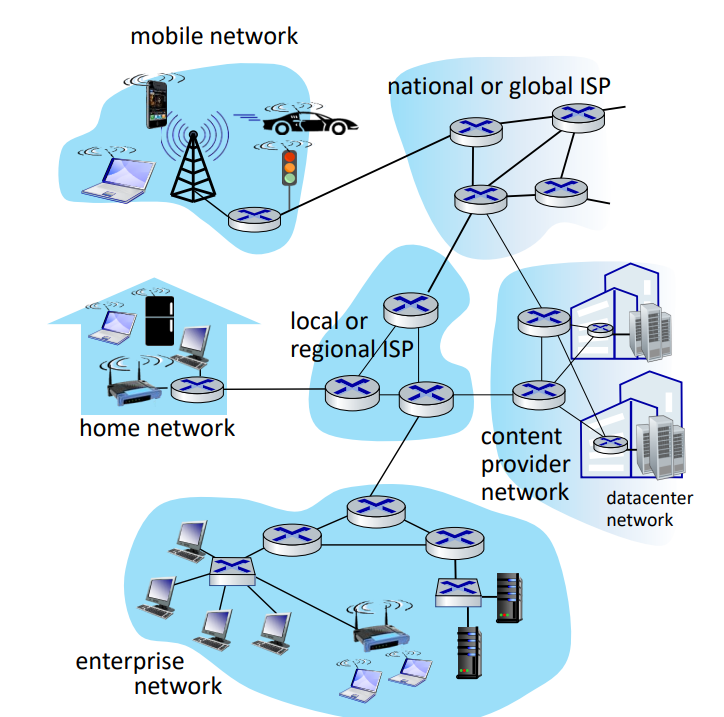
\includegraphics[width = 0.70\linewidth]{Images/1.PNG}
\end{center}
Internet è fisicamente una \textbf{rete connessa}, tuttavia vi sono dei sistemi che permettono di filtrare il traffico (firewall ecc...) per impedire che
ogni nodo della rete sia accessibile da un qualsiasi altro nodo. Internet è quindi una \textbf{rete di reti} che interconnette le reti
degli \textbf{Internet Service Providers} (ISP), cioè quelle entità che forniscono servizi di connettività. Il funzionamento della rete internet è governato
dai \textbf{protocolli di comunicazione}:
\begin{itemize}
    \item Controllano il modo in cui avviene l'invio e il ricevimento dei messaggi
    \item Esempi sono i protocolli HTTP (web), TCP, IP, WiFi, 4G, Ethernet ecc..
\end{itemize}
Protocolli di tipo diverso servono per \textbf{far comunicare dispositivi di tipo diverso}.
Poiché il contesto delle reti è quindi molto eterogeneo, il tutto riesce a funzionare grazie agli \textbf{standard}.
Esistono diversi enti di standardizzazione, tra cui citiamo:
\begin{itemize}
    \item \textbf{RFC}: Request for Comments, documenti
    \item \textbf{IETF}: Internet Engineering Task Force; rilascia le RFC
\end{itemize}
Il compito degli enti di standardizzazione è quello di rilasciare documenti che vanno a definire le caratteristiche
dei protocolli e delle architetture. Possiamo tuttavia vedere internet anche dal punto di vista dei \textbf{servizi}:
internet può essere quindi vista come una \textbf{infrastruttura che offre dei servizi di connettività alle applicazioni distribuite}.
Quindi, internet viene vista come una infrastruttura che \textbf{offre dei servizi di connettività tra nodi diversi}.
\begin{center}
    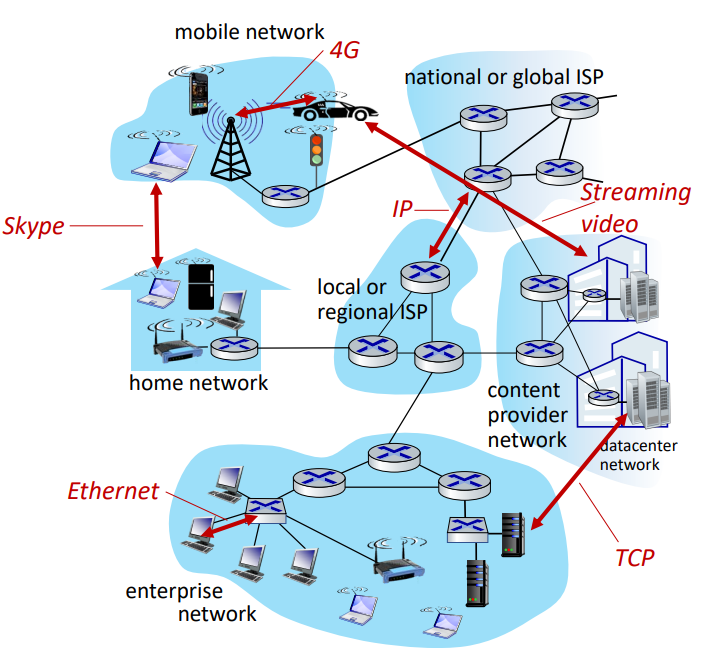
\includegraphics[width = 0.70\linewidth]{Images/2.PNG}
\end{center}
Abbiamo detto che la rete è governata da protocolli, ma \textbf{qual'è la definizione formale di protocollo?}
Una definizione formale può essere la seguente: i \textbf{protocolli} definiscono il \textbf{formato, l'ordine} dei \textbf{messaggi inviati e ricevuti} tra le entità di rete e le
\textbf{azioni intraprese} alla trasmissione e alla ricezione di un messaggio.
\begin{center}
    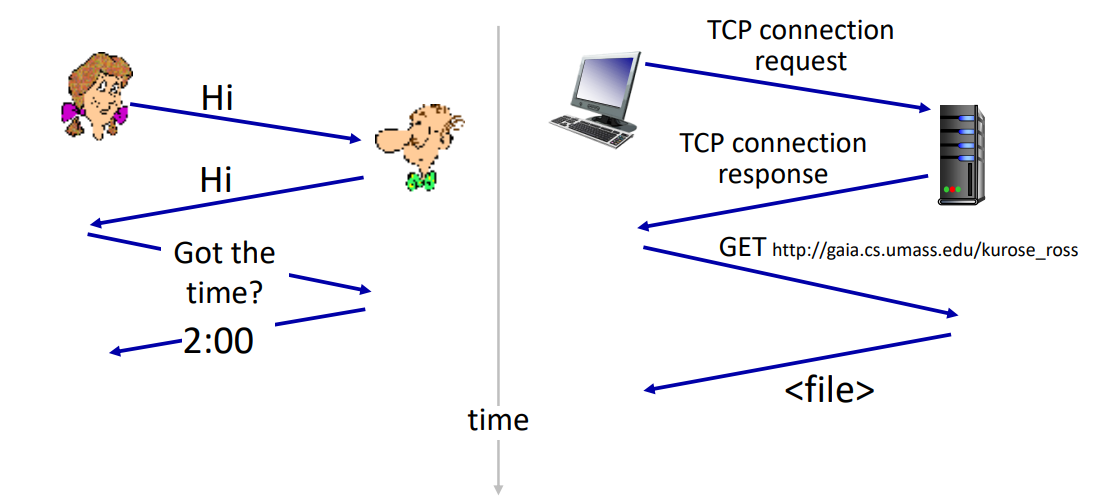
\includegraphics[width = 0.85\linewidth]{Images/3.PNG}
\end{center}
\subsection{Introduzione alla struttura di internet}
La struttura di alto livello di internet si può formalizzare nel seguente modo:
\begin{itemize}
    \item \textbf{Network edge}: il confine della rete, comprende
    \begin{itemize}
        \item \textbf{Hosts}: client e servers
        \item I servers sono spesso in \textbf{data centers}
    \end{itemize}
    È oggetto di dibattito se includere il confine della rete nella struttura di internet o meno; ciò nonostante, rimane comunque
    una componente fondamentale.
    \item \textbf{Access Networks}: Sono tutte quelle reti che servono a raccogliere il traffico generato e destinato per gli utenti.
    Sono quindi i \textbf{punti di accesso alla rete per gli utenti}. Esse possono essere \textbf{cablate oppure wireless}.
    \item \textbf{Network Core}: È l'insieme di tutte quelle reti che sono composte da router interconnessi che permettono di realizzare il concetto di \textbf{rete di reti}.
    Il suo compito è quello di \textbf{connettere le reti di accesso fra di loro} e comprendono tutte quelle reti che, su larga scala, \textbf{permettono il funzionamento di internet}.
\end{itemize}
Ogni componente della struttura di internet viene detto \textbf{segmento}.
\subsubsection{Network Edge}
Il confine della rete è \textbf{popolato dagli host}. Il suo compito principale è quello di inviare i \textbf{pacchetti}
generati dagli host (e quindi dagli utenti). Una visione ad alto livello di questo procedimento è:
\begin{itemize}
    \item Il \textbf{messaggio applicativo} viene generato dall'host
    \item Esso viene \textbf{spezzettato in pezzetti}, chiamati \textbf{pacchetti}, di lunghezza $L$ bits (questa cosa non è sempre vera: ci sono casi in cui i pacchetti hanno lunghezza variabile).
    Ognuno di questi pacchetti presenta una \textbf{intestazione}, cioè un determinato numero di bit che servono per permettere il funzionamento dei protocolli in rete
    \item Una volta generati i pacchetti, essi vengono trasmessi alla rete d'accesso ad un \textbf{tasso di trasmissione} (transmission rate) $R$, il quale è condizionato dalla \textbf{capacità di trasmissione del collegamento}
\end{itemize}
\begin{center}
    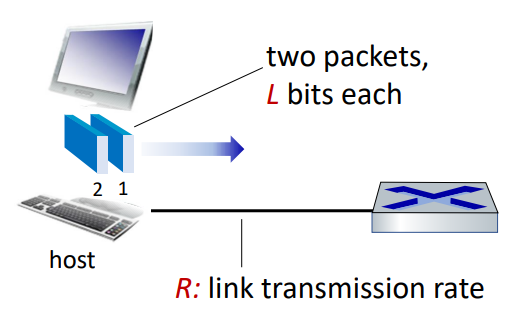
\includegraphics[width = 0.50\linewidth]{Images/4.PNG}
\end{center}
Ogni volta che invio un pacchetto in rete, ho un \textbf{ritardo di trasmissione}, il quale è il tempo necessario per trasmettere un pacchetto di $L$ bit su un collegamento che
ha capacità di trasporto di $R$ bit/sec. Quindi:
$$\textrm{packet transmission delay} = \frac{L \; (bits)}{R \; (bits/sec)}$$
\subsubsection{Access Networks}
Come facciamo a \textbf{connettere gli host a "internet"}? Il compito di effettuare questa connessione è delle
reti di accesso. Esse possono essere:
\begin{itemize}
    \item Reti di accesso \textbf{residenziali}
    \item Reti di accesso \textbf{istituzionali}
    \item Reti di accesso \textbf{mobili}
\end{itemize}
\subsubsection{Network Core}
La Network Core è un insieme di \textbf{maglie di rete interconnesse}, le quali sono fondamentali per effettuare le
operazioni di commutazione dei pacchetti. Esse garantiscono che i pacchetti possano essere trasmessi da un router verso l'altro
attraverso dei collegamenti da una sorgente a una destinazione.
Le reti di core presentano due \textbf{funzionalità fondamentali}:
per spiegarle, dobbiamo prima capire \textbf{come funziona un router}: esso possiede al suo interno una tabella chiamata
\textbf{tabella di inoltro} (forwarding table), che indica verso quale collegamento un pacchetto deve essere instradato in base al valore
della sua intestazione (che quindi contiene, in termini generici, a chi deve essere recapitato questo pacchetto).
L'operazione di \textbf{inoltro} (o \textbf{commutazione di pacchetto}) quindi consiste nell'invio sulla connessione corretta del pacchetto in arrivo (questa operazione viene anche detta \textbf{switching}).
L'inoltro ha \textbf{valenza locale}: ogni router prende in considerazione solo la propria tabella di inoltro locale per decidere dove inoltrare un pacchetto.
Tuttavia, questa operazione non basta per garantire che io possa raggiungere la destinazione corretta; per garantirlo dobbiamo effettuare un'altra operazione che prende il nome di
\textbf{instradamento} (routing). Il routing è un'operazione \textbf{globale} che è utilizzata per determinare \textbf{quale percorso, fra sorgente e destinazione, devono attraversare i pacchetti}.
Ogni singolo router esegui quindi dei \textbf{protocolli} e degli \textbf{algoritmi di routing distribuiti} che hanno l'obbietto di \textbf{popolare le tabelle di inoltro} (viene effettuato tramite algoritmi su grafo).
Poiché gli algoritmi di routing sono \textbf{distribuiti}, essi richiedono lo \textbf{scambio di messaggi e la collaborazione tra i router}.
\begin{center}
    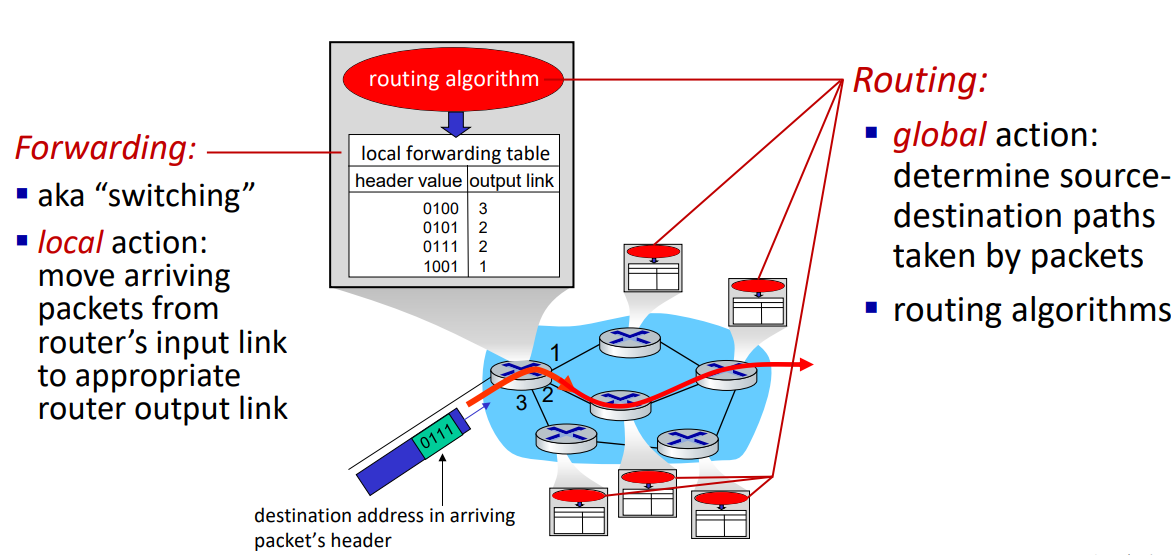
\includegraphics[width = 1\linewidth]{Images/5.PNG}
\end{center}
\subsection{Packet Switching: Store-and-Forward}
Nelle reti a commutazione di pacchetto, \textbf{ogni pacchetto ha vita propria}: una volta che il messaggio viene spezzettato in pacchetti, ognuno di esso
ha un ciclo di vita indipendente dagli altri. La modalità di trasmissione usata da tutte le reti a commutazione di pacchetto è quella del \textbf{store-and-forward}:
quando un pacchetto arriva ad un commutatore per essere commutato, esso deve \textbf{arrivate interamente prima di essere trasmesso al nodo successivo}. Tuttavia, si può pensare
di saltare questo passaggio e trasmettere direttamente ogni bit che arriva su un certo nodo al successivo. Perché non viene fatto nelle reti a commutazione di pacchetto? Il motivo risiede nelle \textbf{intestazioni dei pacchetti}:
infatti, è li che trovo \textbf{tutte le informazioni necessarie per gestire un pacchetto}, quindi devo aspettare che essa venga trasmessa per intero prima di procedere all'invio al nodo successivo.
\begin{center}
    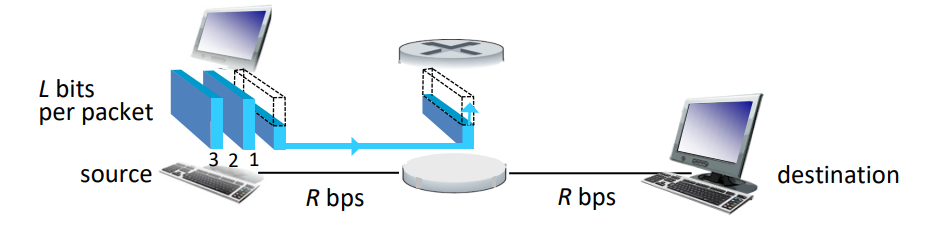
\includegraphics[width =1\linewidth]{Images/6.PNG}
\end{center}
\subsection{Packet-Switching: queuing}
Seppur Store-and-Forward semplifichi di molto la gestione delle reti, esso introduce una problematica che prende il nome di
\textbf{accodamento} (queueing). È una problematica che esiste in tutte le reti e si manifesta quando il \textbf{tasso di arrivo dei pacchetti è superiore al tasso di trasmissione in uscita}.
Nei router e negli switch, i pacchetti si accodano in aree di memoria apposite dette \textbf{buffer}; un pacchetto rimane nel buffer fino a quando non verrà trasmesso.
\begin{center}
    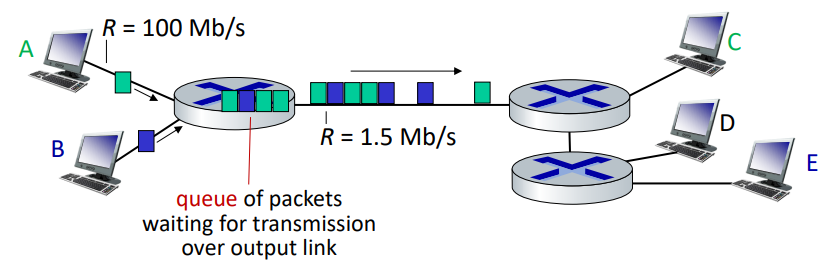
\includegraphics[width =0.90\linewidth]{Images/7.PNG}
\end{center}
Questa è una condizione che può accadere nelle reti a commutazione di pacchetto, tuttavia \textbf{non può essere una situazione sistematica}:
se si verificasse costantemente, la dimensione del buffer \textbf{crescerebbe costantemente} fino a raggiungere la massima dimensione possibile; da quel momento
in poi ogni pacchetto in arrivo porta a una condizione di \textbf{buffer overflow} e andrebbe perso. Quindi, quali sono i problemi che provoca l'accodamento?
\begin{itemize}
    \item \textbf{Buffer overflow} dei buffer dove vengono salvati i pacchetti ancora da trasmettere e susseguente perdita dei pacchetti in arrivo
    \item \textbf{Ritardo di accodamento} dato dall'attesa che il router trasmetta il pacchetto
\end{itemize}
\subsection{Circuit Switching}
La commutazione di pacchetto non è l'unico tipo di commutazione esistente; anzi essa storicamente è posteriore ad un'altro tipo di commutazione
che prende il nome di \textbf{commutazione a circuito}
\begin{center}
    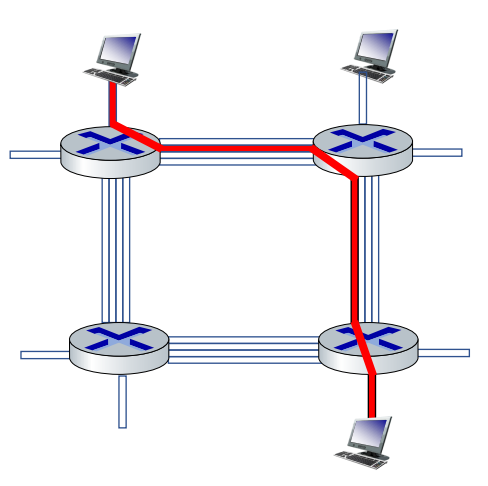
\includegraphics[width =0.45\linewidth]{Images/8.PNG}
\end{center}
Questo tipo di commutazione segue un principio diverso da quella a commutazione di pacchetto: l'elemento fondamentale di questo tipo di rete è il \textbf{circuito} (non esistono i pacchetti in questo tipo di rete).
Tra i vari \textbf{commutatori di circuito} si possono stabilire un certo numero di circuiti.
L'obbiettivo di questo tipo di commutazione è \textbf{destinare i circuiti alla comunicazione tra gli utenti della rete}.
Le risorse di un circuito vengono \textbf{assegnate in maniera esclusiva ad un host} e non possono essere condivise con altri host.
Il vantaggio di questo tipo di commutazione è \textbf{l'assenza di accodamento} data dal completo assegnamento delle risorse di un circuito
ad una sola comunicazione tra sorgente e destinazione.
Viene chiamato \textbf{circuito end-to-end} l'insieme di tutti i circuiti che vengono stabiliti tra sorgente e destinazione.
Uno svantaggio di questo tipo di commutazione è la \textbf{necessità di una fase di setup} in cui vengono allocate le risorse dei circuiti per andare a creare
il circuito end-to-end.
\subsubsection{Packet Switching vs Circuit Switching}
In una commutazione di circuito, le risorse vengono allocate solamente alla comunicazione tra sorgente e destinazione e non esistono
problemi di accodamento. Tuttavia, l'utilizzo delle risorse di rete in questo tipo di comunicazione risulta \textbf{subottimale} rispetto ad una
rete a commutazione di pacchetto. Facciamo un esempio:
\begin{center}
    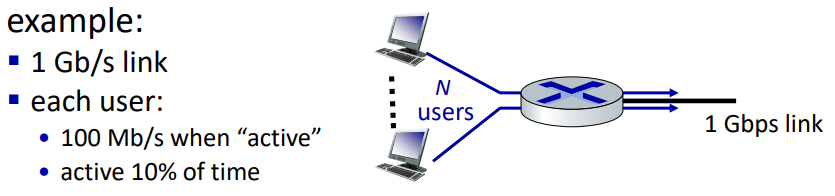
\includegraphics[width =0.75\linewidth]{Images/9.PNG}
\end{center}
\textbf{Domanda: quanti utenti, in queste condizioni, possono rispettivamente accomodare una rete a commutazione di circuito e una rete a commutazione di pacchetto?}
\begin{itemize}
    \item \textbf{Circuit-switching}: 10 utenti
    \item \textbf{Packet-switching}: con 35 utenti, la probabilità che più di 10 utenti siano attivi allo stesso tempo è minore di $0.0004$
\end{itemize}
Quindi una rete a commutazione di pacchetto è sempre la scelta migliore?
\begin{itemize}
    \item Essa è ottima per un traffico di tipo \textbf{"bursty"} (a raffica), cioè in situazioni dove a volte ci sono dati da inviare, a volte no
    \item Permette la condivisione delle risorse di rete
    \item Non richiede setup
\end{itemize}
Tuttavia, se si creano condizioni sfavorevoli, si vanno a creare delle \textbf{situazione di congestione eccessiva della rete}, andando a creare situazioni
di ritardo nella trasmissione dei pacchetti e di buffer overflow. Si rendono quindi necessari \textbf{protocolli di trasmissione affidabili} e meccanismi di \textbf{controllo della congestione}.
È però possibile, visti i vantaggi delle reti a commutazione di circuito, fornire lo stesso tipo di garanzia del servizio anche nelle reti a commutazione di pacchetto?
La risposta è si; esistono delle tecniche che permettono di \textbf{emulare la commutazione di circuito sulle reti a commutazione di pacchetto}, tuttavia sono casi parecchio difficili da gestire.
\subsection{Struttura di internet nel dettaglio}
Gli host sono connessi a internet tramite le \textbf{reti di accesso} fornite da ISPs.
Le reti di accesso devono per forza essere \textbf{interconnesse} per garantire che possa avvenire la comunicazione tra qualsiasi due host della rete (internet è una rete \textbf{connessa}, cioè ogni nodo è raggiungibile da tutti gli altri nodi).
Il risultato dell'evoluzione di internet è una \textbf{struttura gerarchica}; questa evoluzione, tuttavia, non è stata guidata da \textbf{necessità di tipo tecnico} ma di tipo \textbf{economico e politico}.
Vediamo quindi la struttura di internet passo passo: al mondo abbiamo \textbf{milioni} di reti di accesso
\begin{center}
    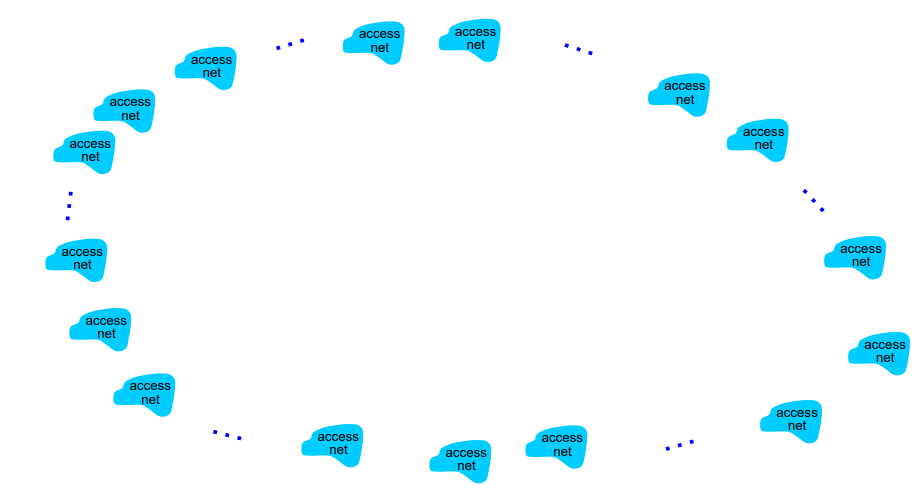
\includegraphics[width =0.85\linewidth]{Images/10.PNG}
\end{center}
L'idea più semplice per interconnetterle è \textbf{connettere ogni ISP agli altri in maniera diretta}, tuttavia...
\begin{center}
    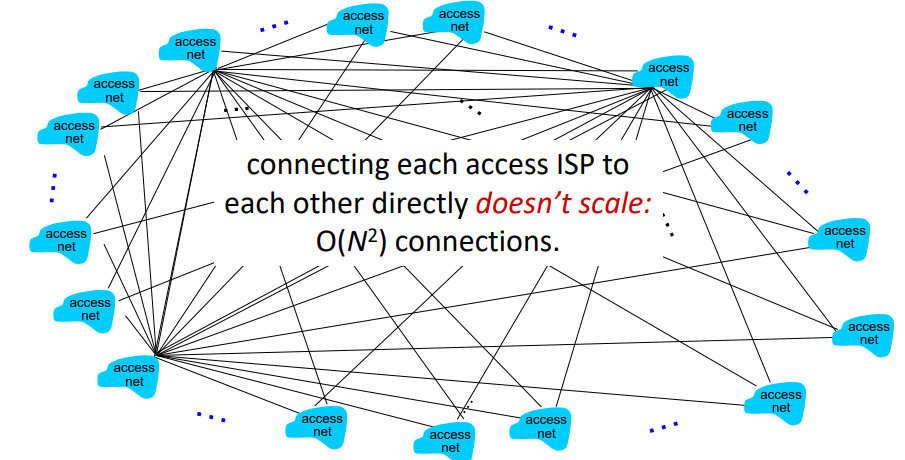
\includegraphics[width =0.85\linewidth]{Images/11.PNG}
\end{center}
Una soluzione alternativa è quella di avere un \textbf{ISP globale} (o di transito) con una rete geograficamente estesa in tutto il mondo, i cui router sono \textbf{interconnessi} e che fornisce connettività alle reti di accesso:
\begin{center}
    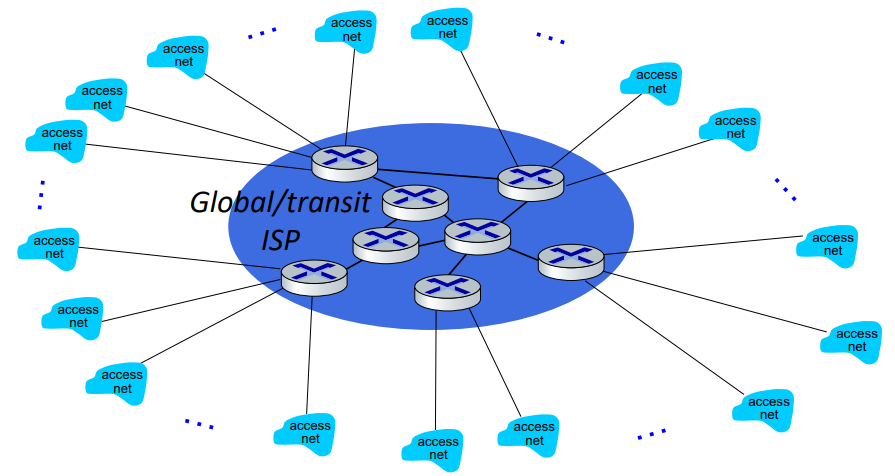
\includegraphics[width =0.85\linewidth]{Images/12.PNG}
\end{center}
Questo approccio tuttavia ha dei problemi:
\begin{itemize}
    \item Richiede una rete estesa \textbf{su tutto il globo}, in modo che possa servire ogni rete di accesso
    \item Richiede un accordo economico tra gli ISP locali e quello globale
    \item Perché ci si dovrebbe limitare ad un solo ISP globale? In effetti, ci potrebbe essere concorrenza fra essi
\end{itemize}
In virtù dell'ultimo punto sopra, si è andata a creare una situazione di questo tipo:
\begin{center}
    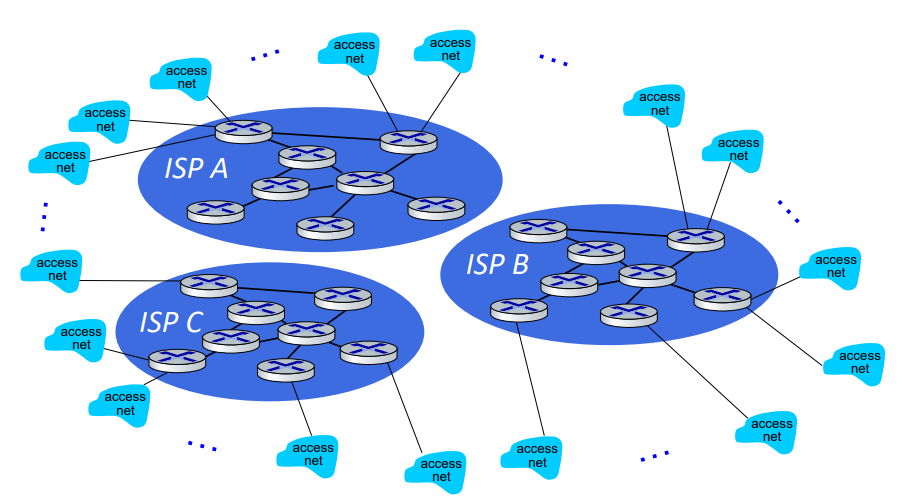
\includegraphics[width =0.85\linewidth]{Images/13.PNG}
\end{center}
si sono andati quindi a creare degli ISPs \textbf{geograficamente estesi} che coprono determinate aree del globo.
Questo genere di ISPs prendono il nome di \textbf{Tier 1 ISPs}.
A questo punto, gli ISPs globali devono creare dei \textbf{peering links} (chiamati così perché \textbf{non sono il frutto di un accordo economico ma di un accordo tra pari})
per creare un'interconnessione tra di loro:
\begin{center}
    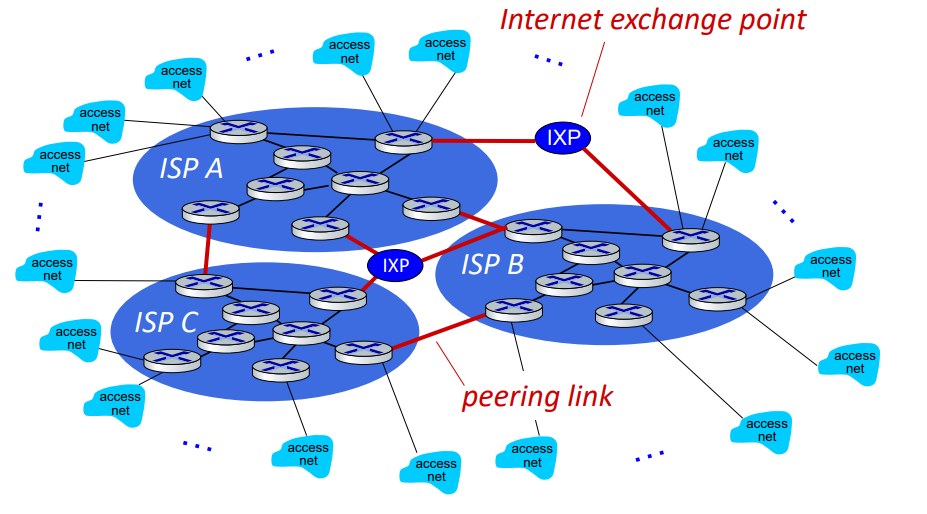
\includegraphics[width =0.85\linewidth]{Images/14.PNG}
\end{center}
Tuttavia, c'è anche un'altra possibilità, cioè quella di avere degli \textbf{Internet Exchange Points} (IXPs), i quali sono dei nodi a cui gli ISPs globali si connettono e che garantiscono
la connessione tra di essi. Tuttavia, tipicamente le reti di acceso non si \textbf{interfacciano direttamente con gli ISPs globali} ma passano tramite \textbf{ISPs regionali}, che hanno una diffusione
più capillare sul territorio. Altro tipo modo in cui le reti di accesso accedono agli ISPs globali è tramite \textbf{multi-homing}, cioè una rete di accesso potrebbe avere \textbf{più collegamenti verso un ISPs globale o regionale};
questo approccio garantisce \textbf{resilienza}
\begin{center}
    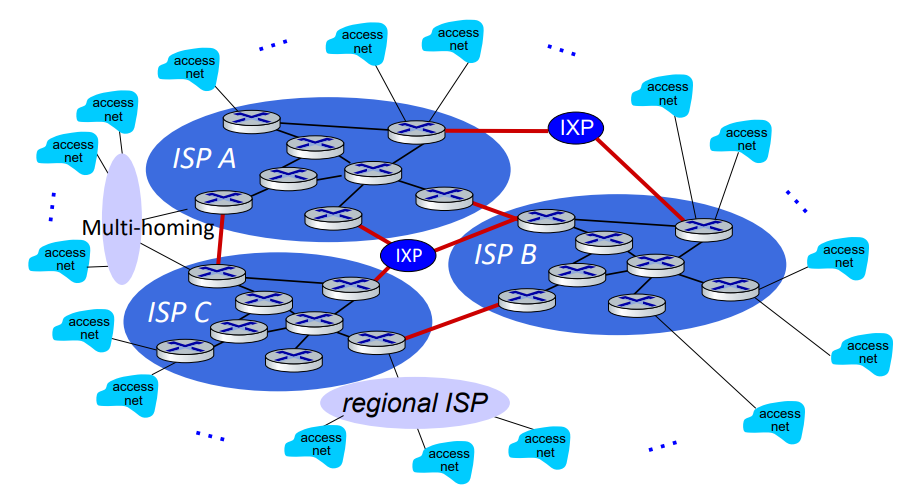
\includegraphics[width =0.85\linewidth]{Images/15.PNG}
\end{center}
Infine, abbiamo le \textbf{reti dei content provider}, che hanno lo scopo di \textbf{fornire contenuto agli utenti}. Per farlo, molto spesso, esse \textbf{bypassano gli ISPs globali} e si interfacciano
direttamente con le reti di accesso.
\begin{center}
    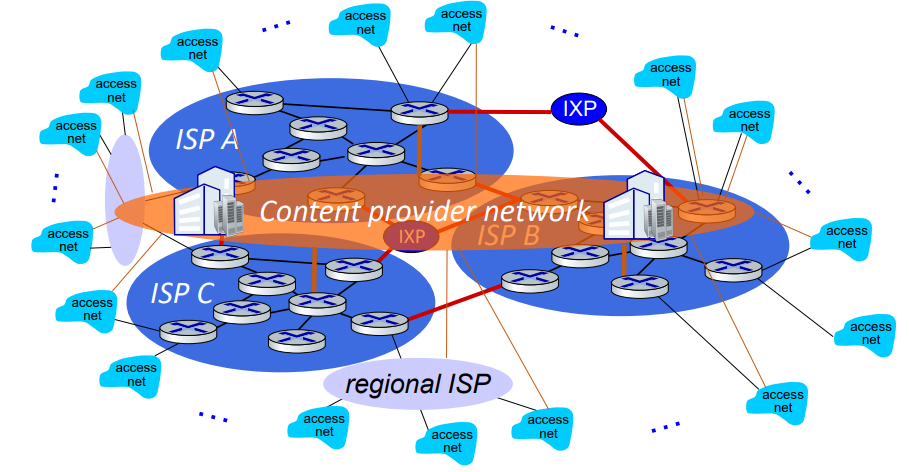
\includegraphics[width =0.85\linewidth]{Images/16.PNG}
\end{center}
Nulla però vieta alle reti dei content provider di accedere anche alle reti degli ISPs globali.
Diamo una versione più generale della gerarchia:
\begin{center}
    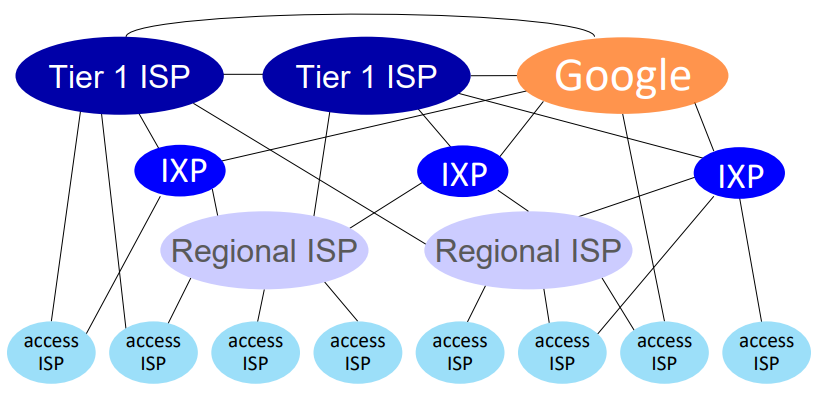
\includegraphics[width =0.85\linewidth]{Images/17.PNG}
\end{center}
Tuttavia, le connessioni possibili \textbf{possono anche non limitarsi a quelle mostrare in figura}.
\subsection{Metriche di performance nelle reti}
Il ritardo e la perdita sono due delle metriche fondamentali per capire la prestazione della rete.
Abbiamo già parlato di \textbf{ritardo di accodamento} e di \textbf{ritardo di trasmissione}, tuttavia essi sono
solo due dei tipi di ritardo che si possono verificare.
\begin{center}
    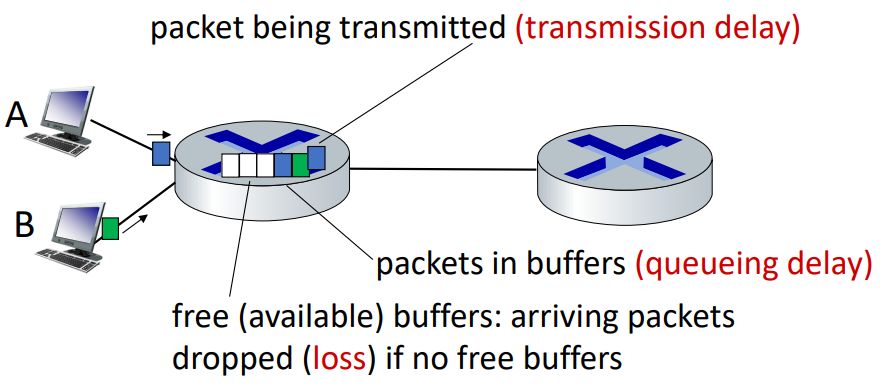
\includegraphics[width =0.70\linewidth]{Images/18.PNG}
\end{center}
Tuttavia ce ne sono delle altre, vediamole tutte: 
\begin{itemize}
    \item \textbf{Ritardo di elaborazione} ($d_{proc}$): quando un pacchetto arriva ad un nodo, devono essere effettuate delle operazioni fondamentali, per esempio \textbf{l'analisi della tabella di inoltro per capire su quale collegamento trasmettere il pacchetto} (lookup).
    Altra operazione è il \textbf{controllo dei bit di errore}: a volte, per colpa di distorsioni o "rumore" sul canale, certi bit di un pacchetto possono essere cambiati (da 0 a 1 e viceversa); il pacchetto quindi risulta malformato. Esistono meccanismi che permettono
    di \textbf{individuare se c'è stato un errore} (e anche di ricostruire il pacchetto originale). Questi metodi sono detti di \textbf{controllo e correzione dell'errore} e richiedono del tempo per essere eseguiti, tendenzialmente nell'ordine dei \textbf{microsecondi} ($10^-6 s$).
    \item \textbf{Ritardo di accodamento} ($d_{queue}$): è il tempo che il pacchetto attende per essere trasmesso. Dipende dal livello di congestione della rete. È tipicamente nell'ordine dei millisecondi
    \item \textbf{Ritardo di trasmissione} ($d_{trans}$): Se abbiamo un pacchetto di lunghezza $L$ che vogliamo trasferire su un collegamento con tasso di trasmissione $R$, allora il ritardo di trasmissione è dato da:
    $$d_{trans} = \frac{L}{R}$$
    \item \textbf{Ritardo di propagazione} ($d_{prop}$): Il ritardo di propagazione è il tempo che necessita un pacchetto per \textbf{propagarsi da un capo all'altro del collegamento}. Questo ritardo dipende dalla lunghezza del collegamento fisico $d$ (espressa in \textbf{metri} (m))
    e dalla \textbf{velocità di propagazione} $s$, che è nell'ordine di grandezza della \textbf{velocità della luce}: $\sim 2 \cdot 10^8 \; m/sec$, e si calcola nel seguente modo:
    $$d_{prop} = \frac{d}{s}$$
\end{itemize}
\begin{center}
    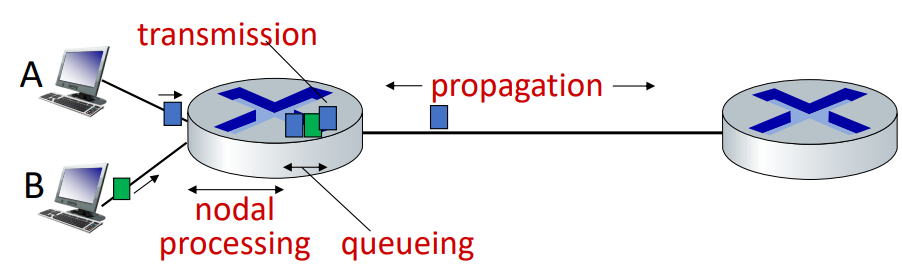
\includegraphics[width =0.70\linewidth]{Images/19.PNG}
\end{center}
Il \textbf{ritardo totale del nodo} (ritardo \textbf{end-to-end}) $d_{nodal}$ è calcolato come la somma di tutti ritardi visti sopra:
$$d_{nodal} = d_{proc} + d_{queue} + d_{trans} + d_{prop}$$
esso è uno delle \textbf{metriche più importanti} e mi permette di valutare le prestazioni della rete. Per calcolare il ritardo ent-to-end bisognerebbe anche tener conto dei \textbf{ritardi introdotti dai sistemi periferici},
che tuttavia non considereremo per questi appunti.
\subsubsection{Ritardo di accodamento e intensità di traffico}
Il ritardo di accodamento ha una caratteristica particolare: mentre tutti gli altri ritardi sono \textbf{analoghi} se considero lo stesso pacchetto trasmesso in due momenti diversi, \textbf{per il ritardo di accodamento non è così}.
Il ritardo di accodamento dipende dallo stato della rete durante la trasmissione. Questo ritardo di solito viene studiato tramite \textbf{metodi statistici}: in particolare, il ritardo di accodamento dipende da un valore che viene chiamato \textbf{intensità di traffico} ("traffic intensity"):
$$\frac{L \cdot \overline{a}}{R} = \frac{\textrm{tasso di arrivo dei pacchetti (bit/s)}}{\textrm{tasso di uscita dei pacchetti (bit/s)}}$$
Dove:
\begin{itemize}
    \item $\overline{a}$ è il \textbf{tasso di arrivo medio dei pacchetti} (pacchetti/s)
    \item $L$ è la \textbf{lunghezza} dei pacchetti (bit/packet)
    \item $R$ è la \textbf{larghezza di banda} del collegamento (bit/s)
\end{itemize}
L'intensità di traffico è \textbf{adimensionale} ed è una quantità non negativa:
\begin{itemize}
    \item Se l'intensità di traffico è \textbf{vicina a 0}, allora il ritardo di accodamento medio sarà piccolo
    \item Se l'intensità di traffico è \textbf{vicina a 1}, allora il ritardo di accodamento medio è grande
    \item Se l'intensità di traffico è \textbf{maggiore di 1}, allora il tasso di arrivo dei pacchetti \textbf{è troppo alto rispetto alla capacità della rete di smaltirli}, quindi il tempo di accodamento medio è \textbf{potenzialmente infinito}
\end{itemize}
\begin{center}
    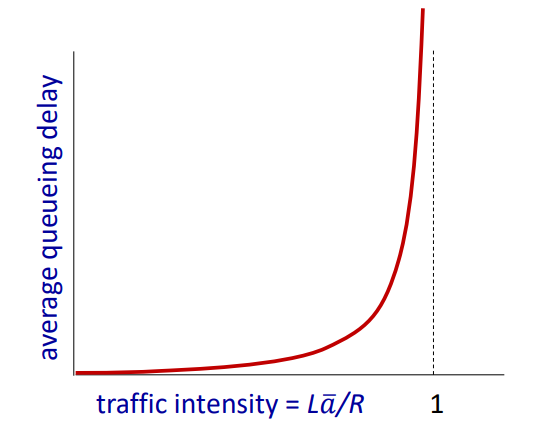
\includegraphics[width =0.50\linewidth]{Images/20.PNG}
\end{center}
\subsubsection{Perdita di pacchetti}
Un'altra metrica di performance fondamentale è la \textbf{perdita di pacchetti}; infatti, idealmente essa dovrebbe essere \textbf{nulla}.
La perdita di pacchetti si verifica quando si ha un buffer overflow sul buffer di accodamento di un nodo.
La perdita di pacchetti può essere mitigata tramite \textbf{meccanismi di ritrasmissione dei pacchetti} da parte del nodo sorgente (tuttavia non è obbligatorio che avvenga).
\begin{center}
    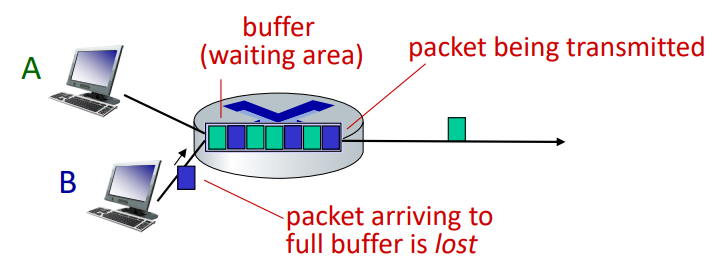
\includegraphics[width =0.70\linewidth]{Images/21.PNG}
\end{center}
Oltre alla perdita per accodamento, \textbf{i pacchetti possono essere scartati dai commutatori} se ci sono stati troppi errori durante la trasmissione oppure se non è previsto un meccanismo di correzione degli errori.
\subsubsection{Throughput}
Il \textbf{throughput} è il \textbf{tasso a cui i bits vengono inviati dal mittente al destinatario}; si calcola in bit/s e viene a volte chiamato \textbf{throughput end-to-end}.
Come si fa a calcolare il throughput?
\begin{itemize}
    \item \textbf{Throughput istantaneo}: tasso di invio \textbf{ad un certo punto nel tempo}
    \item \textbf{Throughput medio}: tasso di invio medio \textbf{su un lungo periodo di tempo}; si può ottenere facendo la media di tutti i valori istantanei o nel seguente modo: supponiamo di voler trasferire un file $F$ dal punto A al punto B; allora il throughput sarà la dimensione del file diviso il tempo che ha impiegato il file ad essere trasferito 
\end{itemize}
Il throughput è una metrica di prestazione "quanto bene" la rete sta andando nella comunicazione tra un mittente ed un destinatario.
\begin{center}
    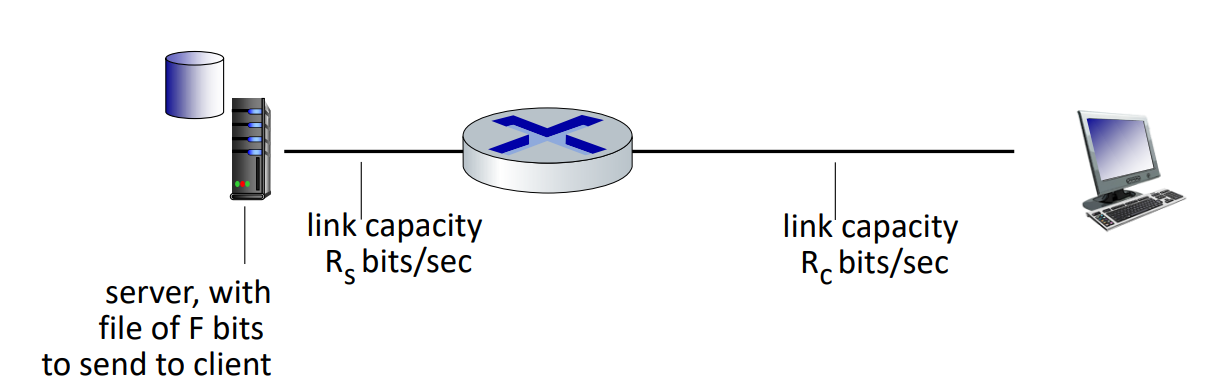
\includegraphics[width =1\linewidth]{Images/22.PNG}
\end{center}
Si possono verificare vari casi:
\begin{itemize}
    \item Se $R_s < R_c$ allora il throughput medio sarà $R_s$. In questo caso, \textbf{non si causerà mai accodamento nel commutatore}
    \item Se $R_s > R_c$ allora il throughput medio sarà $R_c$. In questo caso, potrebbe essere possibile che i \textbf{pacchetti si accodano nel commutatore}
\end{itemize}
In ogni caso, il throughput è vincolato dal collegamento con capacità minore, il quale prende il nome di \textbf{bottleneck link}. Vediamo questo ulteriore scenario:
supponiamo di avere 10 client e 10 server e che essi, per comunicare, passino attraverso un collegamento all'interno della network core con larghezza di banda $R$:
\begin{center}
    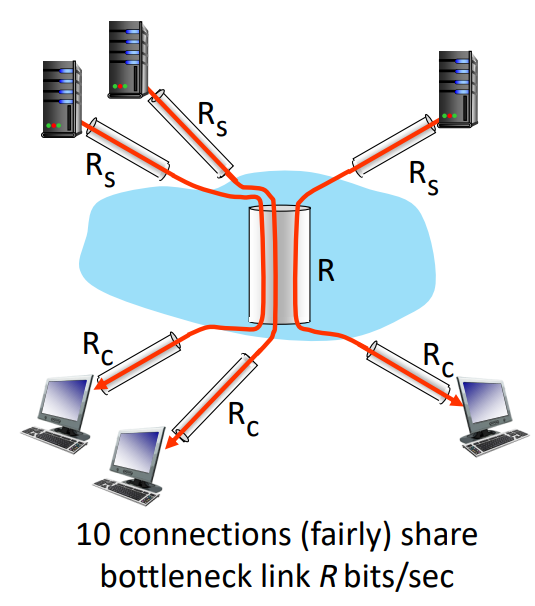
\includegraphics[width =0.40\linewidth]{Images/23.PNG}
\end{center}
In questo caso, il throughput end-to-end per connessione risulta il minimo tra $R_c, R_s,$ e $R/10$, cioè $min\{R_C, R_s, R/10\}$.
Nella pratica, tuttavia, la rete di core ha larghezze di banda \textbf{molto maggiori rispetto ai collegamenti degli hosts}, quindi $R/10$, il più delle volte, sarà comunque molto maggiore di $R_s$ e $R_c$.
Ciò significa che, molto spesso, il bottleneck è dato dai collegamenti di accesso.
\subsection{Strato protocollare e modelli di servizio}
Le reti sono dei sistemi molto complessi con diverse componenti che interagiscono fra loro
\begin{itemize}
    \item Hosts
    \item Routers
    \item Collegamenti di diverso tipo e scopo
    \item Applicazioni
    \item Protocolli
    \item Hardware e Software
\end{itemize}
C'è allora un modo intelligente per \textbf{strutturare e discutere le reti}?
Un modo è una \textbf{struttura a strati}, in cui ogni servizio viene implementato tramite \textbf{azioni interne allo strato} e ogni servizio fa affidamento ai servizi \textbf{appartenenti al livello sottostante per implementare le proprie operazioni e garantirne il funzionamento}.
Inoltre, i vari strati sono \textbf{indipendenti l'uno dall'altro}, nel senso che, in caso di modifiche a come vengono implementati i servizi in uno strato, gli altri strati \textbf{non vengono influenzati dalla modifica}.
L'approccio a strati quindi permette di approcciarsi alla modellazione e alla discussione di sistemi complessi:
\begin{itemize}
    \item La sua \textbf{struttura esplicita} permette l'identificazione e le \textbf{relazioni fra le varia componenti del sistema}. Crea inoltre un \textbf{modello di riferimento a strati} per la discussione
    \item Permette la \textbf{modularizzazione} del sistema e quindi rende più semplice l'aggiornamento e la manutenzione di questo
    \begin{itemize}
        \item I cambiamenti nell'implementazione dei servizi di uno strato sono \textbf{trasparenti al resto del sistema} e quindi non lo influenzano
    \end{itemize}
\end{itemize}
Ciò che è stato definito per internet prende il nome di \textbf{pila (o stack) protocollare di internet} e prevede l'esistenza di 5 diversi strati, numerati dal basso verso l'alto:
\begin{center}
    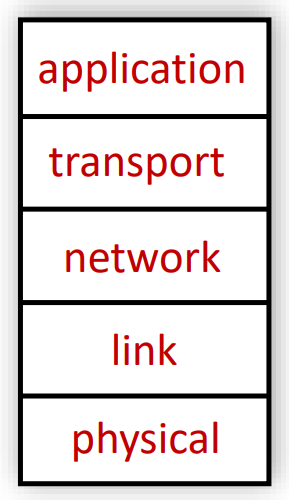
\includegraphics[width =0.15\linewidth]{Images/24.PNG}
\end{center}
Vediamoli nel dettaglio:
\begin{itemize}
    \item \textbf{LIVELLO 5: APPLICATIVO}: Tutti i protocolli volti al supporto alle applicazioni di rete (HTTP, SMTP, DNS ecc..)
    \item \textbf{LIVELLO 4: TRASPORTO}: Ha il compito di effettuare un trasferimento di dati tra macchine che si trovano su reti differenti. Esempio di protocolli a questo livello sono TCP e UDP
    \item \textbf{LIVELLO 3: RETE}: Offre il servizio fondamentale di \textbf{instradamento} tra sorgente e destinazione. Protocollo fondamentale a questo livello è \textbf{Internet Protocol} (IP)
    \item \textbf{LIVELLO 2: COLLEGAMENTO}: Ha il compito di trasferire i dati tra \textbf{due entità di rete adiacenti}, cioè su un collegamento. Protocolli a questo livello sono, per esempio, Ethernet e 802.11(WiFi).
    \item \textbf{LIVELLO 1: FISICO}: Trasporto fisico dei bit su un cavo (o canale radio)
\end{itemize}
\subsubsection{Servizi, Stratificazione e Incapsulamento}
Come si può andare ad implementare i vari protocolli che garantiscono il funzionamento dei servizi ad ogni livello?
Un concetto fondamentale da introdurre a questo scopo è quello dell'\textbf{incapsulamento}: le applicazioni si devono
scambiare messaggi per realizzare i propri servizi, e per farlo devono basarsi sui servizi offerti dal \textbf{livello di trasporto}
\begin{center}
    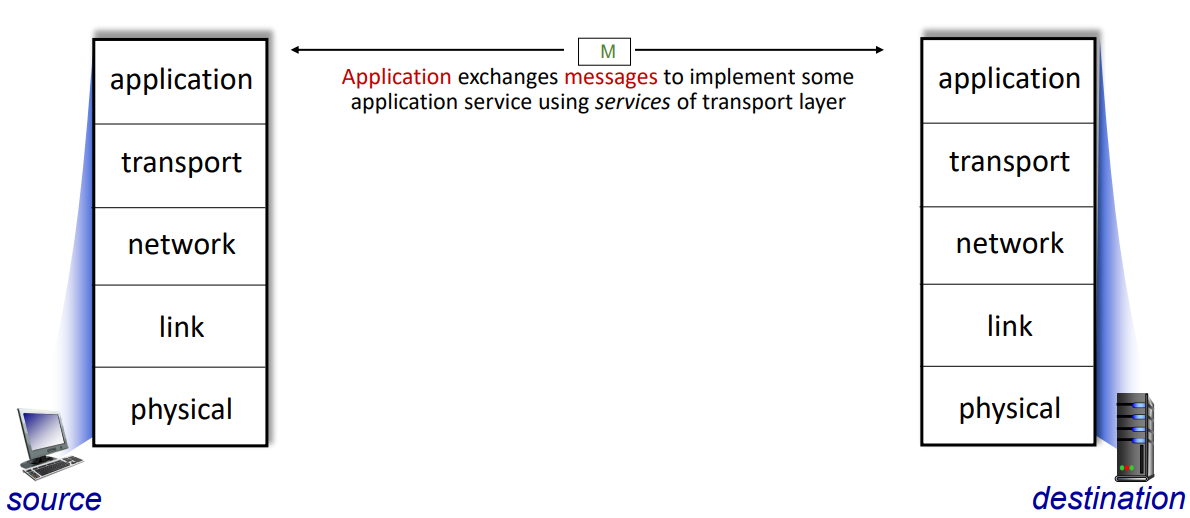
\includegraphics[width =1\linewidth]{Images/25.PNG}
\end{center}
Il messaggio viene quindi passato al livello di trasporto, il quale \textbf{aggiunge un'intestazione (operazione di incapsulamento)} che va ad implementare il servizio a livello di trasporto:
\begin{center}
    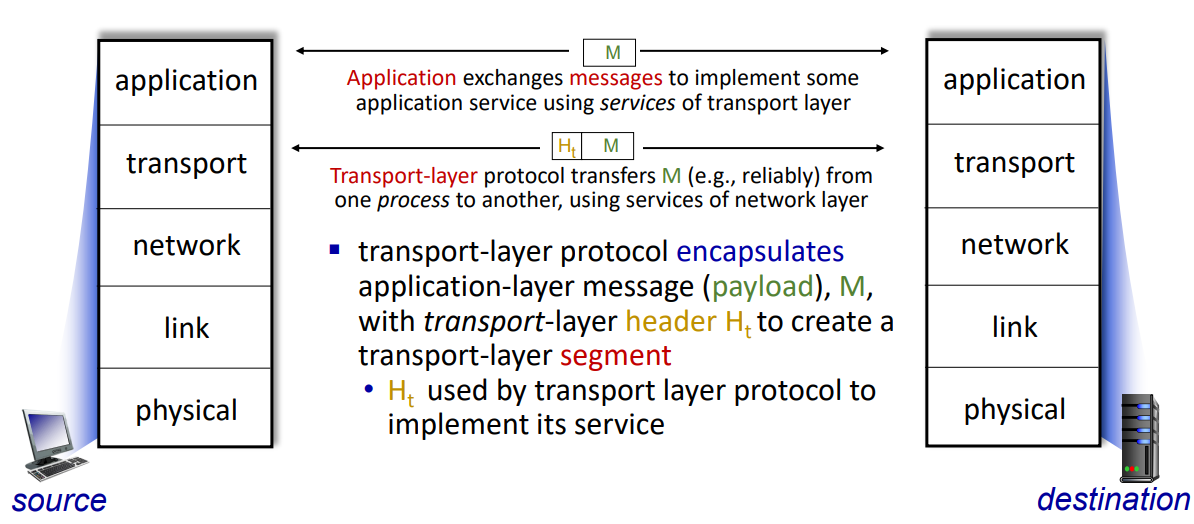
\includegraphics[width =1\linewidth]{Images/26.PNG}
\end{center}
A sua volta, il livello di trasporto usa \textbf{i servizi del livello di rete}, quindi passerò il nuovo \textbf{segmento} al livello di rete, il quale aggiungerà un'ulteriore intestazione:
\begin{center}
    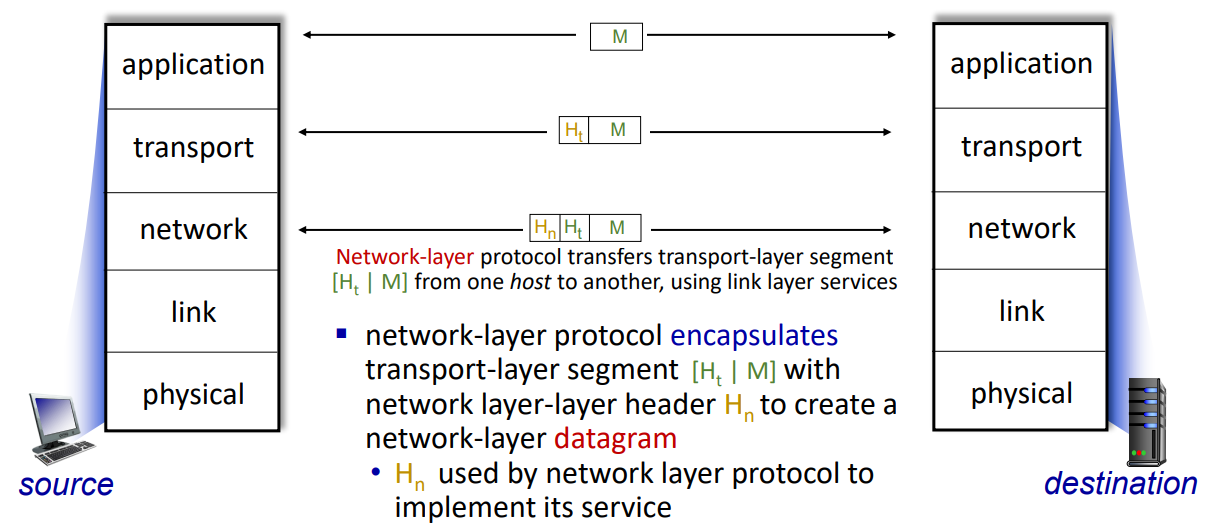
\includegraphics[width =1\linewidth]{Images/27.PNG}
\end{center}
Da notare che a questo livello \textbf{il payload contiene anche l'header del trasporto}, e sarà così anche per le prossime operazioni.
Lo strato di rete si basa sui \textbf{servizi offerti dal livello di collegamento} per implementare i propri, quindi passa il nuovo \textbf{datagramma} ottenuto al livello di collegamento:
\begin{center}
    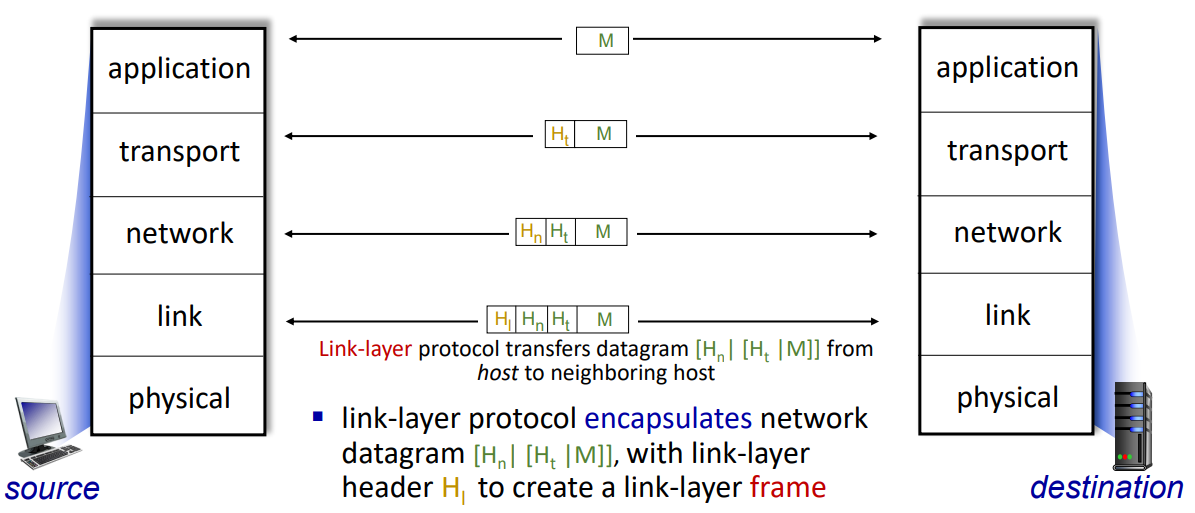
\includegraphics[width =1\linewidth]{Images/28.PNG}
\end{center}
Infine, il pacchetto verrà passato al livello fisico e quindi trasmesso al destinatario.
Come abbiamo già accennato, i pacchetti hanno  nome diverso in strati diversi:
\begin{center}
    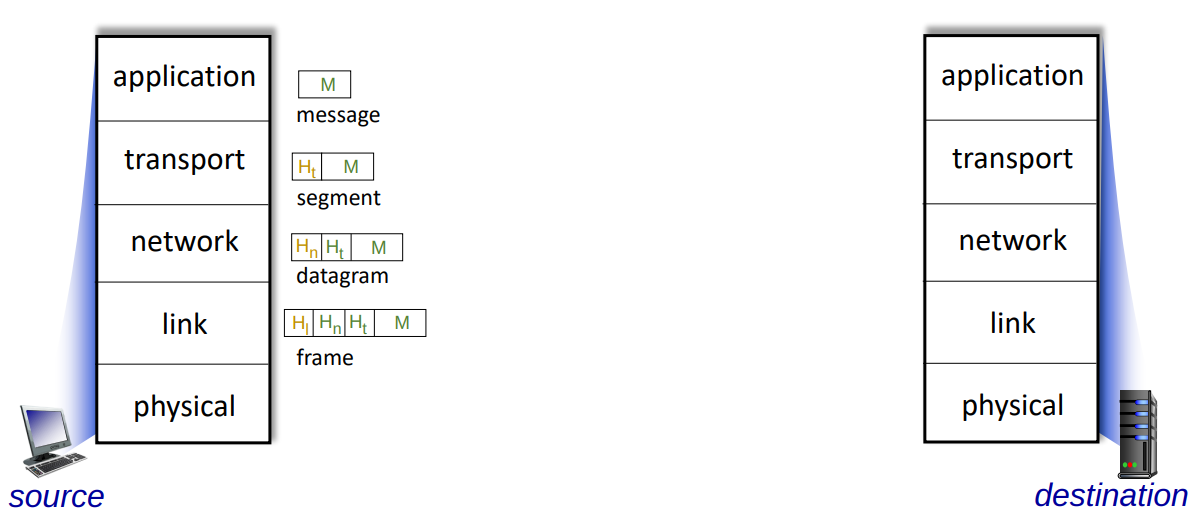
\includegraphics[width =1\linewidth]{Images/29.png}
\end{center}
Man mano che si scende nella pila protocollare, vengono aggiunti nuovi bit di intestazione, i quali servono per \textbf{far funzionare i servizi di rete}.
L'insieme di tutti i bit aggiunti da ogni strato prende il nome di \textbf{overhead} del pacchetto. Poiché il throughput viene misurato \textbf{a livello applicativo},
non si avrà mai, a livello pratico, \textbf{una misura di throughput massima} poiché non vengono contati i bit di overhead. Dopo l'operazione di \textbf{incapsulamento} del messaggio
e di trasmissione su cavo fisico, avviene sul sistema ricevente un'operazione di \textbf{decapsulamento} del messaggio:
\begin{center}
    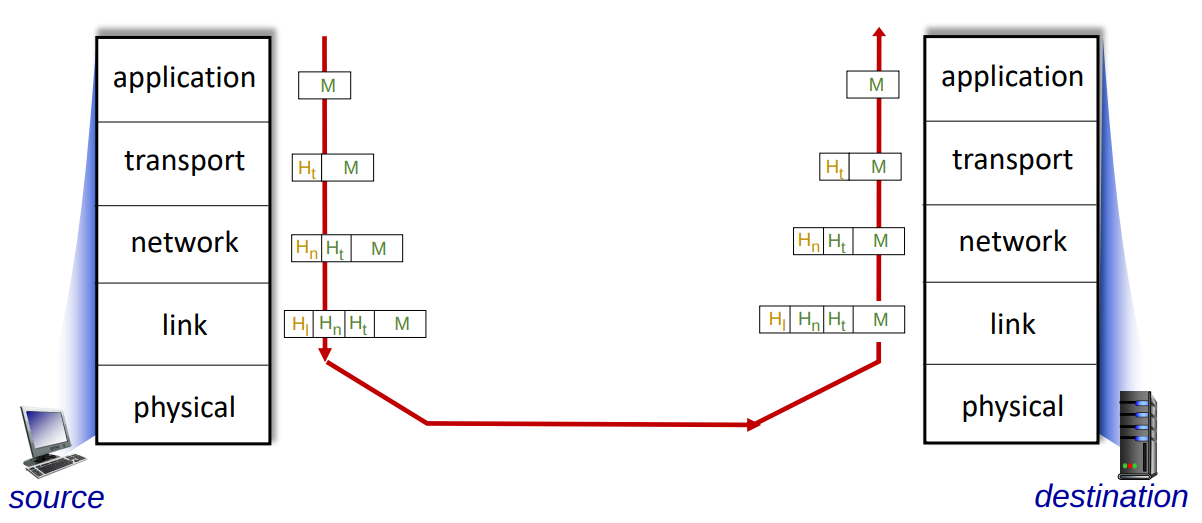
\includegraphics[width =1\linewidth]{Images/30.png}
\end{center}
I sistemi periferici sono sempre in grado di interpretare tutti gli strati della pila protocollare; questo però non è vero per i \textbf{commutatori}, che "parlano" fino al \textbf{livello 2} se sono
degli \textbf{switch} e fino al \textbf{livello 3} se sono dei \textbf{router}:
\begin{center}
    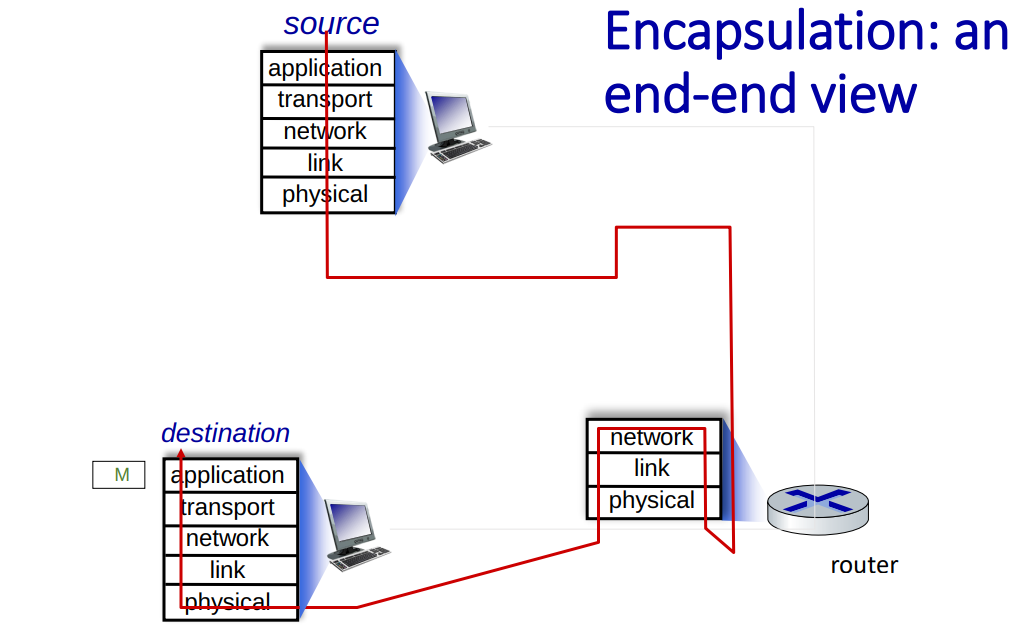
\includegraphics[width = 0.80\linewidth]{Images/31.png}
\end{center}
\section{Strato applicativo: Domain Name System}
Lo strato applicativo ha la funzione di interfacciare e fornire servizi di connettività per i \textbf{processi delle applicazioni}. Il numero
di protocolli presenti in questo strato è altissimo; in questi appunti, tuttavia, ci concentreremo sul protocollo \textbf{DNS}, il quale è una funzionalità chiave di internet, in particolare
se si pensa ad esso come \textbf{fornitore di servizi web}. Quando inseriamo il \textbf{nome} di un sito nel browser, ciò che è avviene è lo scatenamento di un meccanismo che permette al computer
di ottenere \textbf{l'indirizzo IP} (quindi l'indirizzo a livello di rete) associato al server che deve fornire la pagina web richiesta. Per ottenere questo indirizzo IP, non si può pensare di conoscere
ogni indirizzo esistente, quindi è necessario un meccanismo che ci permette di reperirlo: il \textbf{Domain Name System} (DNS). Il DNS permette di effettuare la traduzione dall'\textbf{host name} (i nomi "human readable" dei siti)
all'indirizzo IP del server associato che dovrà fornire al richiedente il contenuto. Come funziona quindi la traduzione? Essa sfrutta la \textbf{gerarchia} di un numero molto elevato di \textbf{server DNS} (che prendono anche il nome di \textbf{name servers}),
i quali andranno a \textbf{risolvere} (tradurre) gli host name in indirizzi IP. Poiché il DNS è un protocollo a livello applicativo, la complessità di questa operazione si trova \textbf{interamente ai confini della rete}.
Il DNS funziona nel seguente modo:
\begin{center}
    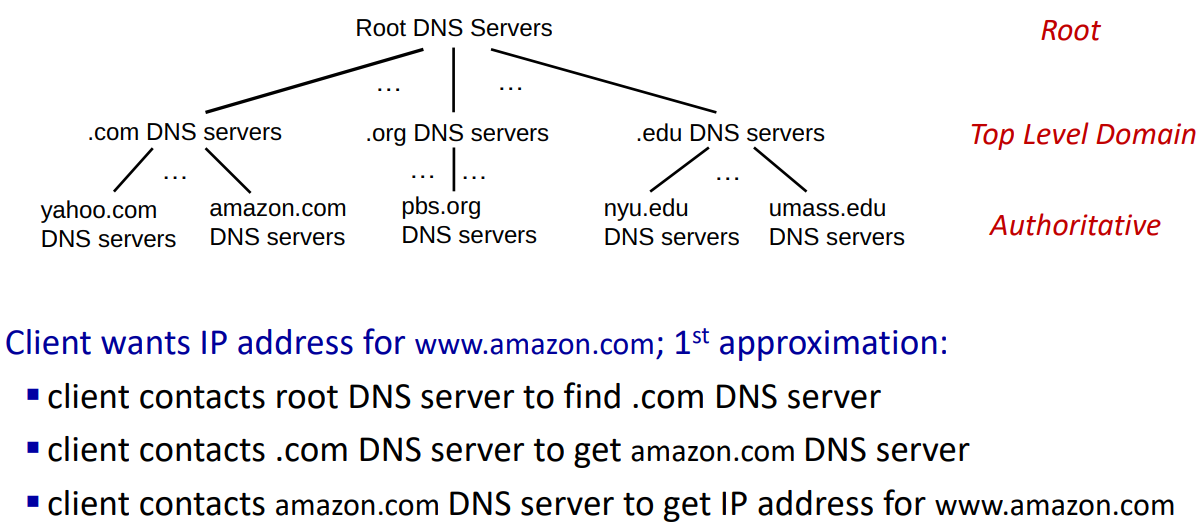
\includegraphics[width = 0.90\linewidth]{Images/32.png}
\end{center}
abbiamo quindi un sistema distribuito che si articola su \textbf{3 livelli}:
\begin{itemize}
    \item \textbf{Root DNS servers}: sono la radice dell'albero gerarchico
    \item \textbf{Top Level Domain (TLD) DNS Servers}: sono responsabili della risoluzione dei \textbf{Top Level Domains}(TLDs); come per esempio .com, .net, .it, ...
    \item \textbf{Authoritative DNS Servers}: Responsabili di risolvere gli indirizzi per i vari domini autoritativi (es. amazon.com, google.com ecc...)
\end{itemize}
Questi 3 livelli collaborano tra loro per risolvere il nome richiesto.
\subsection{Root DNS Servers}
I root DNS server stanno alla radice del sistema DNS e senza la loro esistenza \textbf{è fondamentale per l'esistenza del web}.
In tutto, esistono 13 root name servers "logici", gestiti da \textbf{12 provider differenti}; a loro volta ognuno di questi root dns server è replicato
più volte nel globo. È fondamentale avere repliche dei root name server geograficamente sparse che possono essere acceduti dai vari luogo del mondo.
\begin{center}
    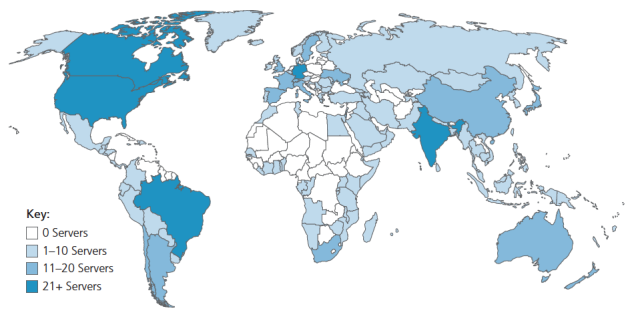
\includegraphics[width = 0.70\linewidth]{Images/33.png}
\end{center}
\subsection{Top Level DNS servers e Authoritative DNS servers}
Ogni TLD DNS server è responsabile per la risoluzione dei TLD, inclusi quelli nazionali (.it, .de. .pl, ...).
I DNS server autoritativi invece è importate specificare che \textbf{possono essere mantenuti dall'organizzazione che detiene il dominio}
oppure \textbf{possono essere mantenuti da un service provider}. Il loro compito è di risolvere le richieste relative a tutte le pagine appartenenti
al loro dominio.
\subsection{Local DNS name servers}
Quando vi è la necessità di contattare il DNS per risolvere un dominio,la prima cosa che viene fatta è contattare il \textbf{DNS server locale}, a cui viene
demandata di fatto questa risoluzione. Il DNS server locale ha un ruolo fondamentale: esistono DNS server locali forniti da ISP, che di solito sono l'opzione di default,
tuttavia un utente può benissimo cambiare il proprio DNS server locale ad uno fornito da un'organizzazione terza. Il DNS server locale tendenzialmente fornisce due servizi:
\begin{itemize}
    \item Mantiene una cache delle associazioni nome-indirizzo IP. Questa cache viene costruita a partire dalle varie richieste dei sistemi terminali e di solito le associazioni
    vengono mantenute per 2 giorni. Il DNS server locale quindi risponderà direttamente alle richieste del client, senza quindi interpellare la gerarchia del DNS, se il nome richiesto è presente
    nella sua cache.
    \item In caso il nome richiesto non sia presente in cache, il DNS server locale procederà ad inoltrare la richiesta alla gerarchia del DNS; una volta ottenuta risposta, procederà a comunicarla al client
\end{itemize}
Ogni richiesta al DNS prende il nome di \textbf{query}.
\subsection{DNS name resolution: Iterated query}
Ci sono due modi per effettuare query al DNS.
Il modo che prende il nome di \textbf{query iterativa} è quello che viene usato più spesso.
In questo metodo, il local DNS server ha \textbf{il maggior carico} dal punto di vista delle richieste da servire.
\begin{center}
    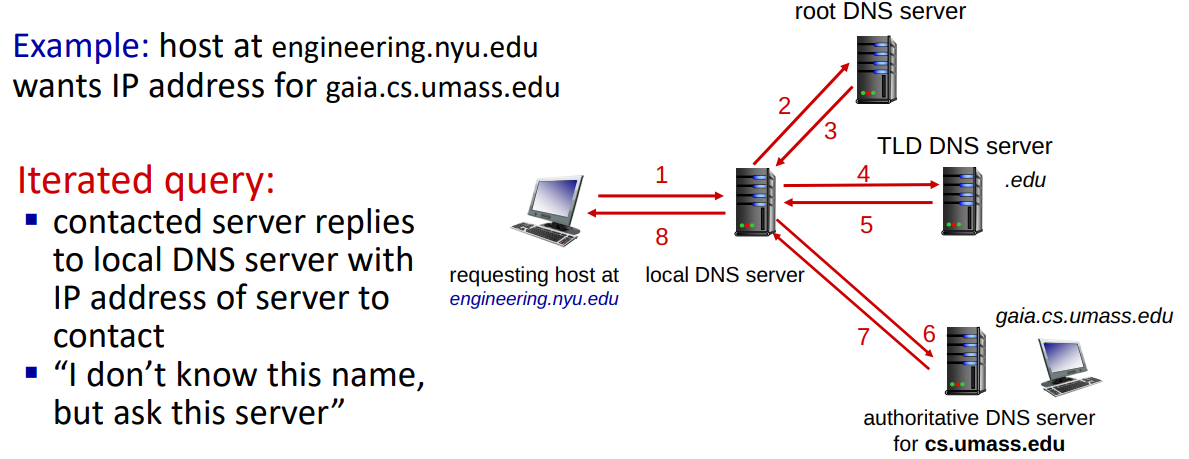
\includegraphics[width = 1\linewidth]{Images/34.png}
\end{center}
\newpage \noindent
Analizziamo nel dettaglio ogni passaggio:
\begin{enumerate}
    \item L'host chiede al DNS server locale di risolvere un certo nome in un indirizzo IP
    \item Il DNS server locale chiede al DNS server root di risolvere il nome
    \item Il DNS server root indica al server DNS server locale quale TLD DNS server può risolvere la sua richiesta
    \item Il DNS server locale chiede al TLD DNS server indicato di risolvere il nome
    \item Il TLD DNS server indica al server DNS locale quale DNS server autoritativo può risolvere la sua richiesta
    \item Il DNS server locale chiede al server DNS autoritativo di risolvere il nome
    \item Il DNS server autoritativo restituisce l'indirizzo IP associato al nome indicato
    \item Il DNS server locale restituisce l'indirizzo IP al client
\end{enumerate}
Ogni passaggio di questo processo è inoltre \textbf{trasparente all'utente}.
\subsection{DNS name resolution: recursive query}
In una query ricorsiva, la risoluzione viene effettuata, in modo gerarchico, dal DNS server di livello superiore.
Il peso delle richieste quindi grava sulla \textbf{struttura gerarchica del DNS}.
\begin{center}
    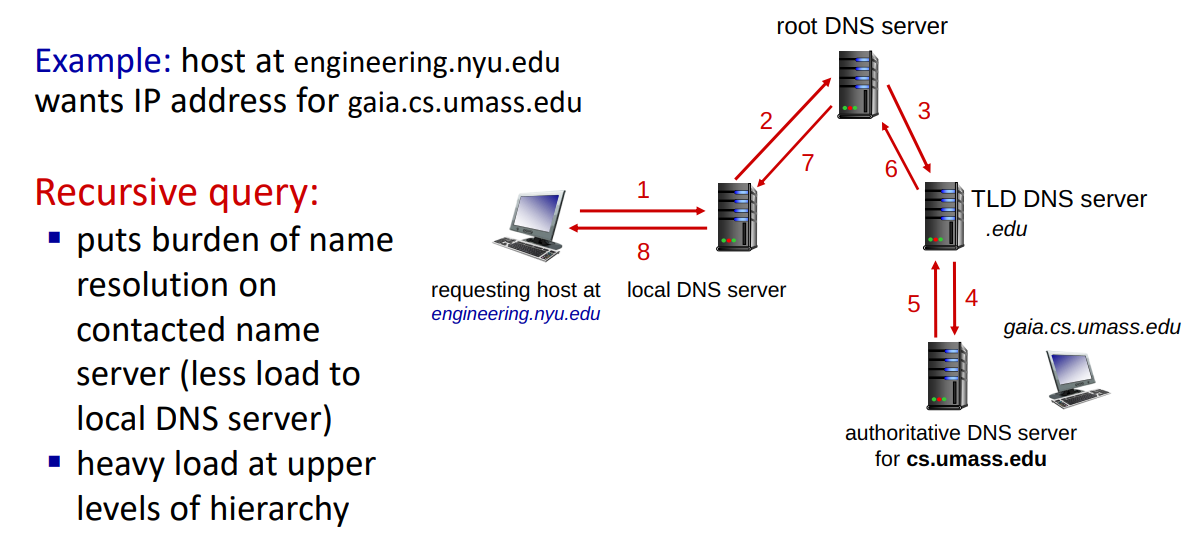
\includegraphics[width = 1\linewidth]{Images/35.png}
\end{center}
Vediamo ogni passo in dettaglio:
\begin{enumerate}
    \item Il client chiede al DNS server locale di risolvere il nome
    \item Il DNS server locale chiede al DNS server di root di risolvere il nome
    \item Il DNS server di root chiede al TLD DNS Server corrispondente di risolvere il nome
    \item Il TLD DNS server chiede al DNS server autoritativo corrispondente di risolvere il nome
    \item Il DNS server autoritativo restituisce l'IP richiesto al TLD DNS server
    \item Il TLD DNS server restituisce la risposta ottenuta al root DNS server
    \item Il root DNS server restituisce la risposta ottenuta al DNS server locale
    \item Il DNS server locale restituisce la risposta ottenuta al client
\end{enumerate}
Solitamente, questo meccanismo non si utilizza poiché tendenzialmente i TLD DNS server, per loro natura, si trovano a gestire
un alta quantità di traffico, quindi un meccanismo di risposta ricorsivo porrebbe ulteriore peso su di essi. Si tende quindi
a cercare di mantenere il peso sui DNS server locali, i quali tendenzialmente gestiscono una quantità di traffico molto minore.
\section{Livello di trasporto}
I servizi del livello di trasporto offrono:
\begin{itemize}
    \item \textbf{comunicazione logica} tra processi su host diversi, cioè processi su macchine diversi possono comunicare come se fossero direttamente connessi fra loro
    \item Le azioni effettuate dai protocolli di trasporto nei sistemi periferici sono:
    \begin{itemize}
        \item \textbf{Mittente}: il livello di trasporto deve prendere i messaggi applicativi, eventualmente \textbf{dividerli in parti più piccole}, incapsularli in quelli che prendono il nome di \textbf{segmenti}
        \item \textbf{Destinatario}: il livello di trasporto \textbf{riassembla i segmenti} per ricostruire il messaggio originale e poi passa il messaggio ricostruito al livello applicativo
    \end{itemize}
\end{itemize}
Come si differenzia il servizio di comunicazione tra processi offerto dal livello di trasporto dal servizio offerto dal livello di rete?
\begin{itemize}
    \item A \textbf{livello di rete}, abbiamo una comunicazione logica tra \textbf{hosts}
    \item A \textbf{livello di trasporto}, estende la comunicazione logica offerta dal livello di rete, migliorandola a una comunicazione tra \textbf{processi su host differenti}  
\end{itemize}
\subsection{Sockets}
Una \textbf{socket} è un "varco" che permette ai processi a livello applicativo di comunicare con il livello di trasporto e di inviare i messaggi verso destinatari
usando lo stack protocollare di internet. Quando quindi un processo deve mandare un messaggio in rete, \textbf{lo fa passare attraverso una socket}; vengono poi sfruttati i servizi
offerti dal livello di trasporto per fare in modo che il messaggio sia recapitato \textbf{ad un'altra socket dal lato del destinatario} (ci sono quindi almeno sempre due socket in una comunicazione tra processi).
Dal punto di vista formale, una socket è \textbf{un'interfaccia} che permette di interfacciare il livello applicativo con il livello di trasporto. La cosa particolare della socket è che, da un lato la parte della socket
che si \textbf{interfaccia con i processi applicativi} può essere controllata da chi sviluppa l'applicazione (può aprirla, chiuderla, ...), dall'altro la parte che si interfaccia con il livello di trasporto è \textbf{controllata dal sistema operativo},
il quale implementa lo stack protocollare.
\begin{center}
    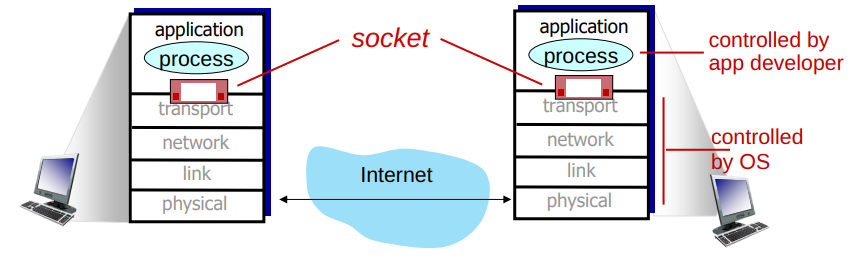
\includegraphics[width = 1\linewidth]{Images/36.png}
\end{center}
\begin{center}
    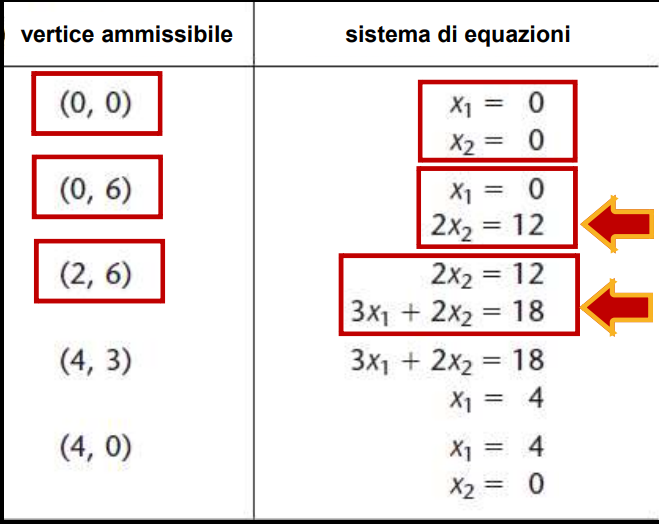
\includegraphics[width = 1\linewidth]{Images/37.png}
\end{center}
\begin{center}
    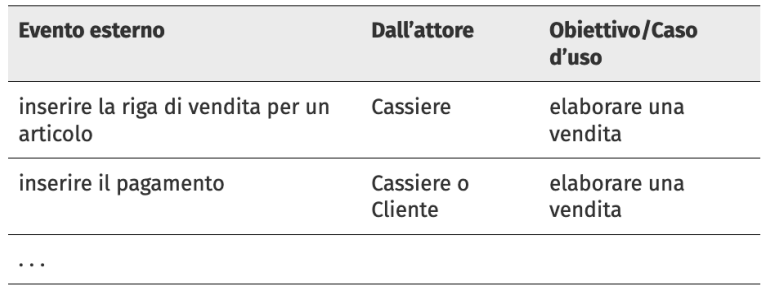
\includegraphics[width = 1\linewidth]{Images/38.png}
\end{center}
\subsection{I principali protocolli di trasporto}
Vi sono due principali protocolli di trasporto:
\begin{itemize}
    \item \textbf{Transmission Control Protocol (TCP)}: Fornisce un servizio di \textbf{consegna dei dati affidabile e in ordine}.
    Offre meccanismi di \textbf{controllo della congestione, controllo di flusso} e di \textbf{inizializzazione della connessione} (TCP è un protocollo \textbf{connection oriented}).
    TCP è adatto alle applicazioni dette \textbf{elastiche}, cioè poco sensibili al ritardo ma \textbf{molto sensibile alla perdita di pacchetti}
    \item \textbf{User Datagram Protocol (UDP)}: Protocollo di trasporto "\textbf{best-effort}" il quale è un'estensione "senza fronzoli" del protocollo IP. 
    Il protocollo è di tipo \textbf{connectionless} ed è adatto alle applicazioni dette \textbf{real-time}: poco sensibili
    alla perdita di pacchetti (in un certo grado) ma \textbf{molto sensibili al ritardo}
\end{itemize}
Nessuno dei due protocolli \textbf{garantisce qualcosa in termini di ritardo}, cioè nessuno dei due garantisce che i pacchetti saranno
consegnati con un ritardo massimo di $n$ secondi. Allo stesso modo, nessuno dei due protocolli garantisce nulla riguardo alla \textbf{banda}: nessuno dei due
garantisce che la comunicazione avvenga a certi bit/s.
\subsection{Multiplexing e Demultiplexing}
Quando si parla di Multiplexing in generale si parla di un'operazione che porta ad unire \textbf{più flussi} in un unico flusso.
Nel caso specifico del livello di trasporto, dobbiamo garantire che il servizio di multiplexing/demultiplexing sia \textbf{garantito} poiché mi permette
di \textbf{estendere logicamente la comunicazione ai processi}. 
\begin{center}
    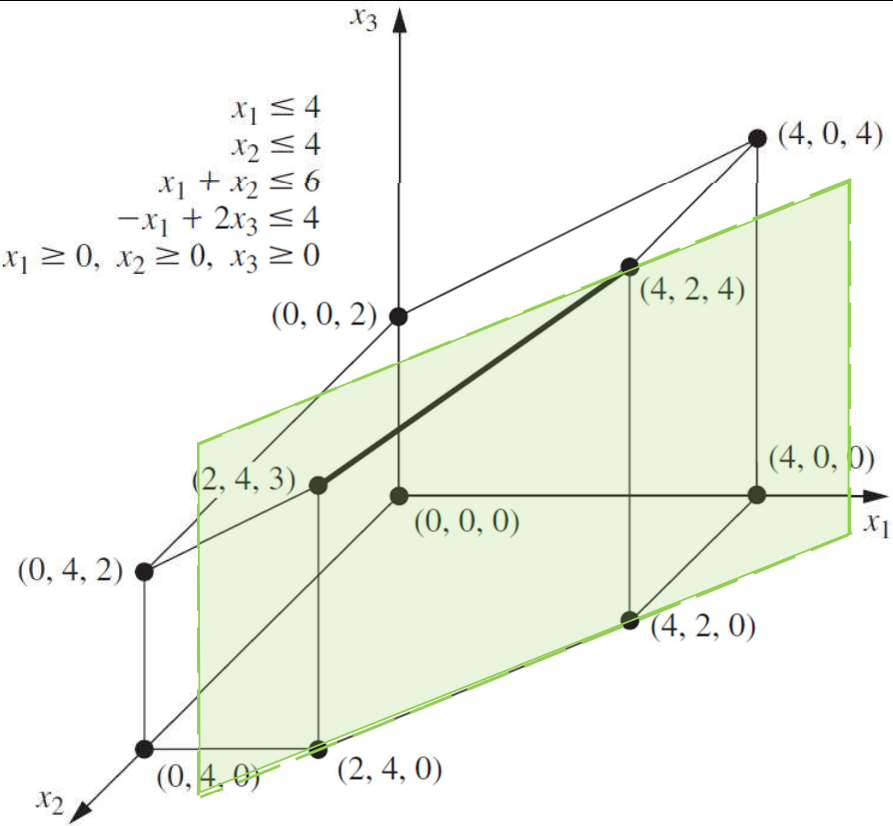
\includegraphics[width = 0.90\linewidth]{Images/39.png}
\end{center}
\begin{center}
    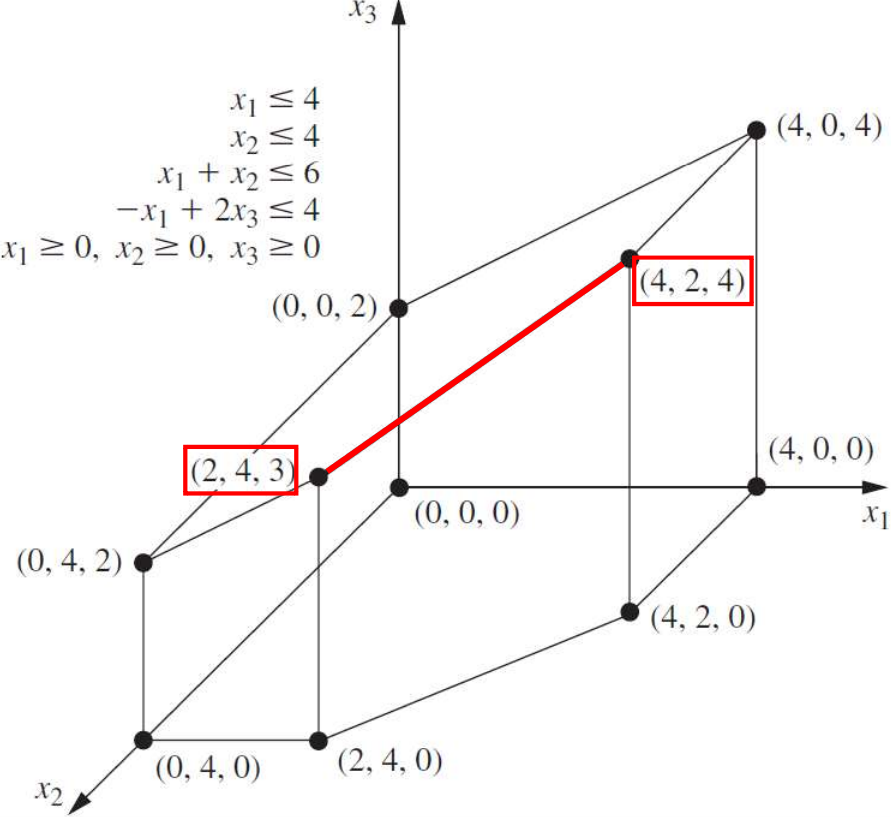
\includegraphics[width = 0.90\linewidth]{Images/40.png}
\end{center}
quindi, l'operazione di multiplazione \textbf{porta ad aggiungere un header ai messaggi provenienti dai processi}, in modo tale che essi siano \textbf{distinguibili} una volta che arrivano al livello di rete; il quale \textbf{non ha conoscenza di quale processo ha generato quale segmento}
ma si preoccupa solamente di consegnare il pacchetto \textbf{all'host corretto}. L'informazione che permette di distinguere i pacchetti è la \textbf{porta di destinazione}. Il livello di trasporto si vedrà recapitati segmenti, dal livello di rete, che avranno
nel loro header dell'informazione relativa alla porta di destinazione; l'operazione di \textbf{demultiplazione} permette, a livello di trasporto, di inoltrare \textbf{verso la socket corretta} segmenti diretti verso \textbf{processi differenti}.
In particolare, l'operazione di \textbf{demultiplazione} funziona nel seguente modo:
\begin{itemize}
    \item L'host riceve i \textbf{datagrammi IP}:
    \begin{itemize}
        \item Ogni datagramma ha un indirizzo IP sorgente e un indirizzo IP destinatario
        \item Ogni datagramma trasporta un \textbf{segmento del livello di trasporto}
        \item Ogni segmento ha una \textbf{numero di porta sorgente e il numero della porta di destinazione}
    \end{itemize}
    \item L'host mittente usa \textbf{l'indirizzo IP e il numero di porta} per inviare i segmenti alla socket appropriata
\end{itemize}
\subsubsection{Connectionless demultiplexing}
Quando si va a creare una socket, \textbf{bisogna specificare attraverso su quale porta essa è raggiungibile}.
La socket di destinazione è \textbf{univocamente identificata} da una coppia di valori:
\begin{enumerate}
    \item \textbf{L'indirizzo IP di destinazione}
    \item \textbf{Il numero della porta di destinazione}
\end{enumerate}
Quando l'host destinatario riceve un segmento UDP:
\begin{itemize}
    \item Controlla il numero della porta di destinazione nel segmento
    \item Invia il segmento UDP alla socket con quella porta
\end{itemize}
I datagrammi IP/UDP con \textbf{la stessa porta di destinazione e stesso indirizzo IP di destinazione}, anche se da indirizzi IP sorgenti differenti e/o con differenti numeri di porta sorgente, saranno
\textbf{inviati alla stessa socket} dell'host destinatario.
\begin{center}
    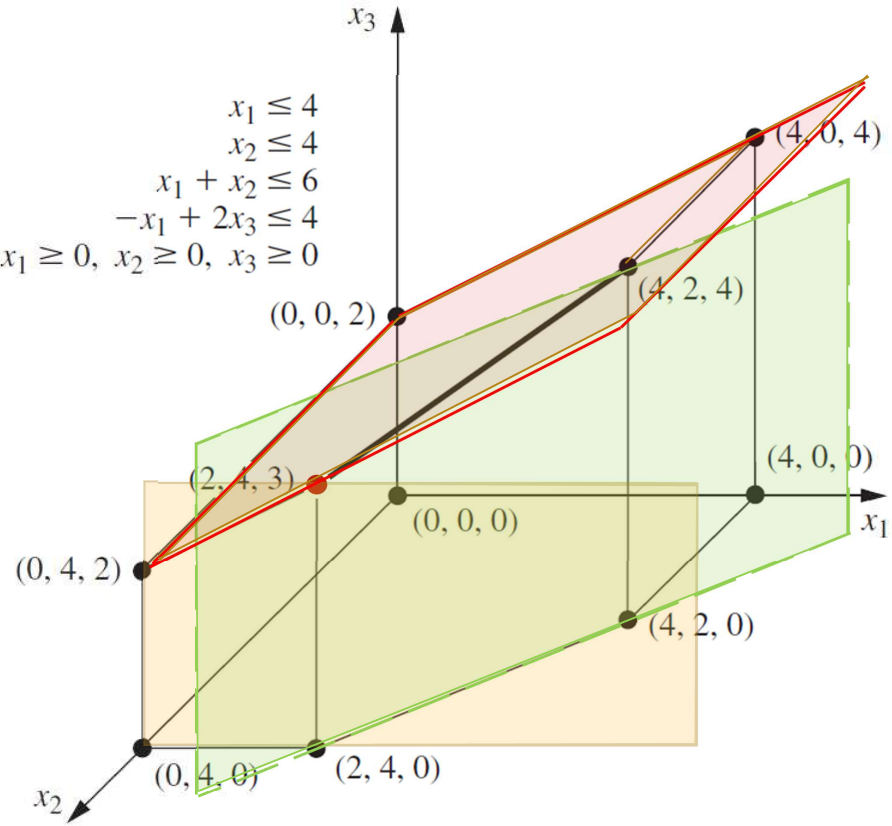
\includegraphics[width = 0.90\linewidth]{Images/41.png}
\end{center}
\subsubsection{Connection-oriented demultiplexing}
A differenza dei protocolli connectionless, una socket è qui identificata \textbf{da una quadrupla}:\
\begin{itemize}
    \item \textbf{Indirizzo IP sorgente}
    \item \textbf{Numero di porta sorgente}
    \item \textbf{Indirizzo IP destinatario}
    \item \textbf{Numero della porta di destinazione}
\end{itemize}
Quando viene effettuata la demultiplazione, allora \textbf{tutti e 4 i valori} verranno usati per inviare il pacchetto alla socket corretta.
Ciò significa che qui si avrà \textbf{una socket dedicata ad ogni connessione}. I server \textbf{possono supportare più socket TCP simultaneamente} e:\
\begin{itemize}
    \item Ogni socket è identificata da una sua quadrupla
    \item Ad ogni socket è \textbf{associato un diverso client comunicante}
\end{itemize}
\begin{center}
    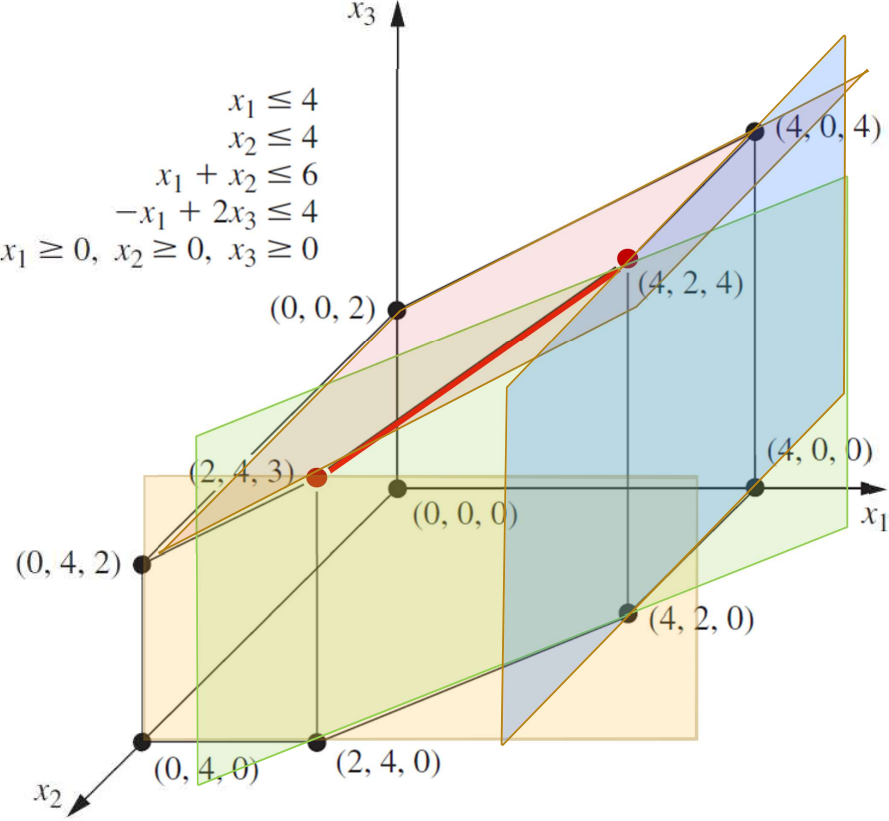
\includegraphics[width = 0.90\linewidth]{Images/42.png}
\end{center}
\subsection{User Datagram Protocol (UDP)}
\textbf{User Datagram Protocol} (UDP) è, di fatto, un'estensione "senza fronzoli" e "minimale" del protocollo IP.
UDP fornisce un servizio di trasporto \textbf{"best effort"}, quindi i segmenti di UDP potrebbero essere:
\begin{itemize}
    \item Persi 
    \item Consegnati in disordine all'applicazione
\end{itemize}
È un \textbf{protocollo connectionless}:
\begin{itemize}
    \item Nessun "handshaking" (inizializzazione della connessione) tra il mittente e il destinatario
    \item Ogni segmento UDP viene gestito indipendentemente dagli altri
\end{itemize}
Perché è necessaria l'esistenza  di UPD?
\begin{itemize}
    \item Nessuna necessità di stabilire una connessione (il che può aggiungere ritardi)
    \item È \textbf{semplice}: nessuno stato di connessione al mittente e al destinatario
    \item \textbf{Dimensioni dell'intestazione piccole}
    \item \textbf{Nessun controllo di congestione}
    \begin{itemize}
        \item UDP può \textbf{trasmettere quanto veloce si vuole}
        \item Può funzionare in casi di congestione della rete (più o meno, comunque fatica in caso di congestione molto elevata)
    \end{itemize}
\end{itemize}
L'header di UDP ha la seguente struttura:
\begin{center}
    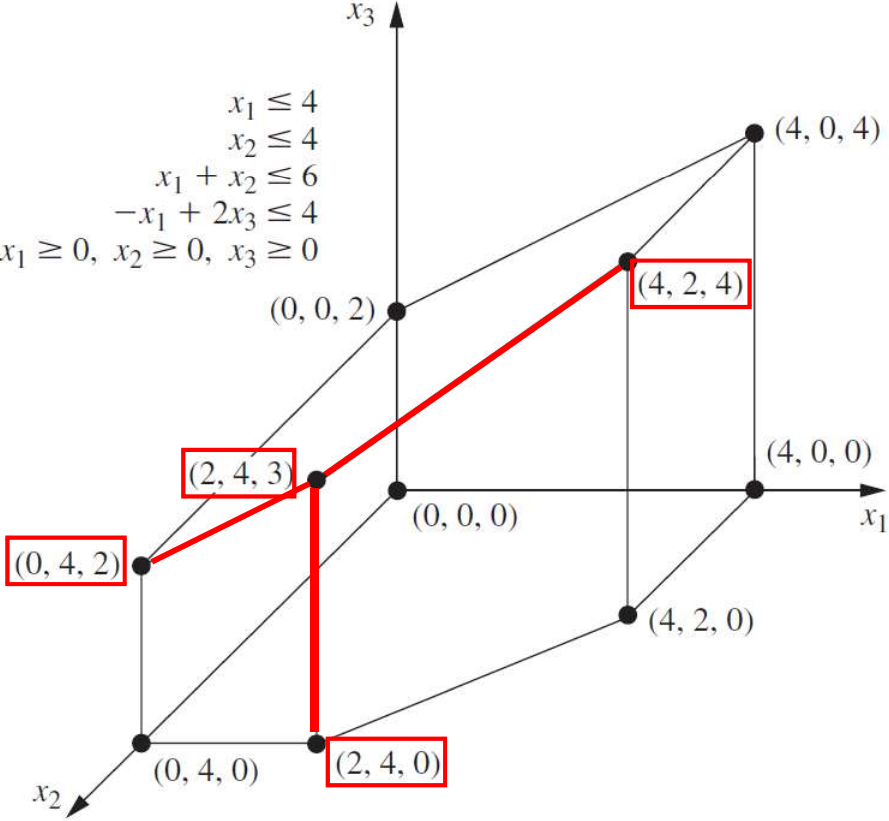
\includegraphics[width = 0.80\linewidth]{Images/43.png}
\end{center}
Facciamo qualche considerazione:
\begin{itemize}
    \item L'header è quindi di \textbf{64 bit}, ed ogni campo è lungo \textbf{16 bit}.
    \item Posso avere $2^{16} - 1$ possibili porti di sorgente e destinazione (la porta con tutti 0 non è tendenzialmente una porta valida)
    \item Includendo l'header, al più posso avere $2^{16} - 1$ byte differenti in un segmento UDP
    \item Il checksum si calcola nel seguente modo: si considerino gruppi di 16 bit del segmento; si sommino modulo 2 e si faccia il complemento di essa.
    Lato destinatario, si effettua la stessa operazione e poi si somma con il checksum: se si ottengono tutti 0 allora non ci sono stati errori.
\end{itemize}
\subsection{Principi del trasferimento dati affidabile}
Per servizio di dati affidabile si intende un servizio di trasporto in cui i dati \textbf{vengono consegnati senza perdite e senza errori}.
Dal punto di vista astratto vogliamo avere la seguente situazione:
\begin{center}
    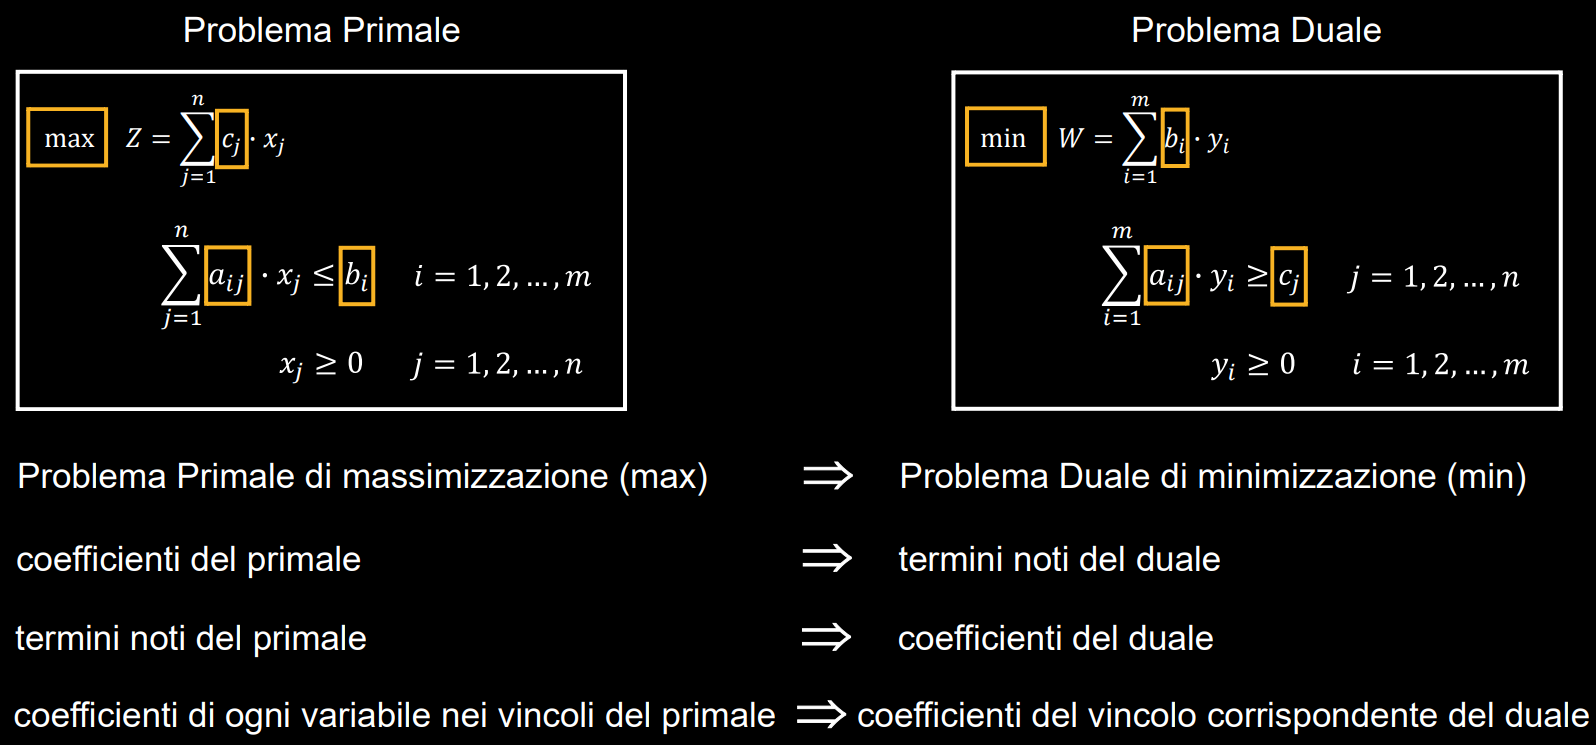
\includegraphics[width = 0.70\linewidth]{Images/44.png}
\end{center}
Tuttavia, nella realtà \textbf{il canale è sempre inaffidabile per definizione}: il protocollo IP è un protocollo "best-effort" e quindi non offre
garanzie sulla consegna, dovremo quindi \textbf{andare ad implementare dei meccanismi di trasporto che rendano la consegna affidabile}:
\begin{center}
    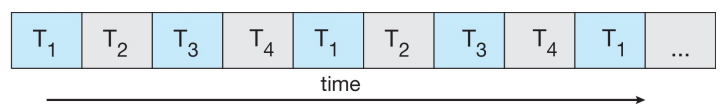
\includegraphics[width = 1\linewidth]{Images/45.png}
\end{center}
Abbiamo poi un ulteriore problema: il mittente e il destinatario \textbf{non conosco lo stato l'uno dell'altro} a meno che \textbf{non sia comunicato tramite messaggio}.
Consideriamo una \textbf{rete ideale}, cioè che non introduce:
\begin{itemize}
    \item Bit di errore
    \item Scarto di segmenti
    \item Segmenti fuori sequenza
\end{itemize}
Il livello di trasporto \textbf{allora non dovrà correggere nulla e il protocollo stesso sarà triviale}: il mittente invia i segmenti in sequenza (uno dopo l'altro) e il ricevente li riceve
senza nessun ulteriore controllo
\begin{center}
    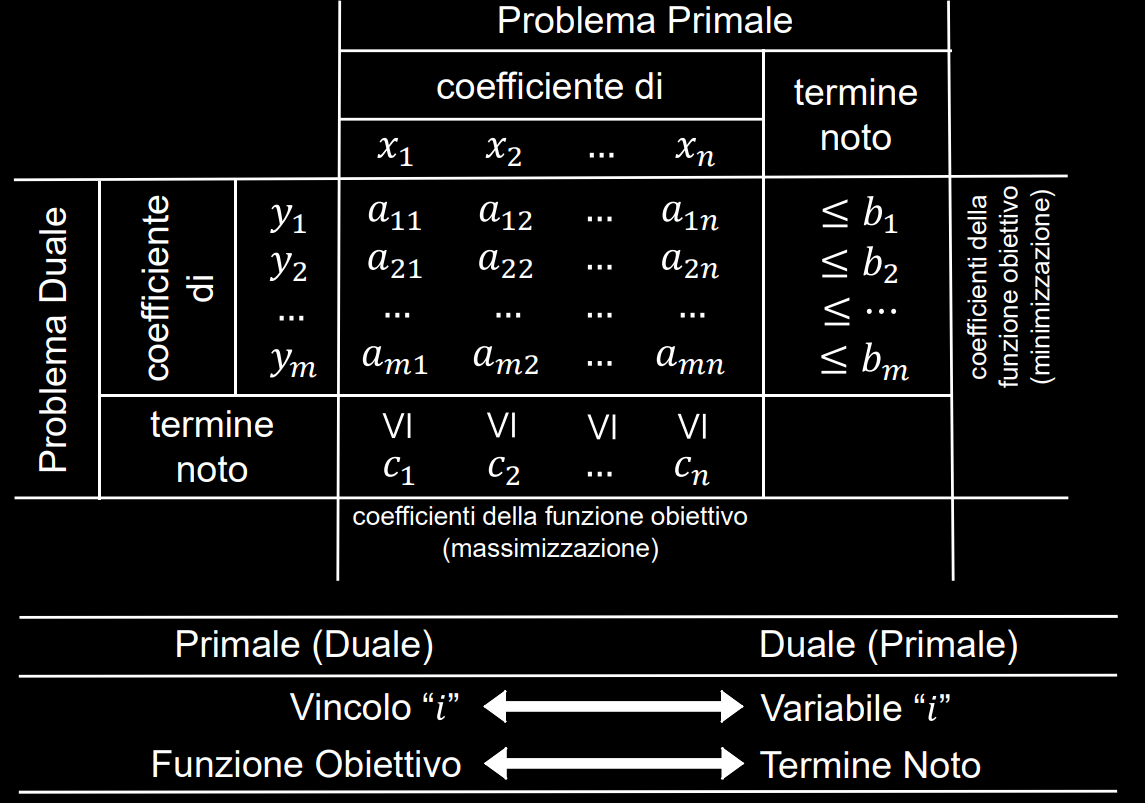
\includegraphics[width = 0.60\linewidth]{Images/46.png}
\end{center}
Sfortunatamente, le reti ideali non esistono. In una rete con errori, è possibile introdurre \textbf{riconoscimenti positivi} (ack) e \textbf{riconoscimenti negativi} (nack).
\begin{center}
    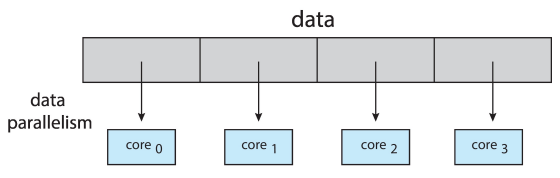
\includegraphics[width = 0.80\linewidth]{Images/47.png}
\end{center}
Un algoritmo di invio molto semplice allora potrà essere il seguente: \newline
\begin{algorithm}[H]
\DontPrintSemicolon
\eIf{ack} {
    $M_{i+1}$
} {
    \If{nack} {
        $M_i$
    }
    \If(\tcp*[h]{problema!}){?} {
        something
    }
}
\end{algorithm}
\noindent
Se la rete è \textbf{soggetta ad errori} anche \textbf{gli ack possono essere soggetti ad errori}, quindi stiamo ipotizzando, con questo algoritmo, che \textbf{la perdita o la corruzione di ack non avvenga}, cosa
che in realtà può accadere nelle reti reali. Un modo per mitigare questo problema è \textbf{ritrasmettere il messaggio se l'ack è corrotto}.
Tuttavia, neanche questo funziona! Non ho un meccanismo per capire se \textbf{un messaggio è duplicato o meno}. Possiamo mitigare ulteriormente questo problema nel seguente modo:
se i \textbf{segmenti sono numerati con un numero di sequenza nell'intestazione}, non c'è il rischio di non sapere se un messaggio è duplicato o meno
\begin{center}
    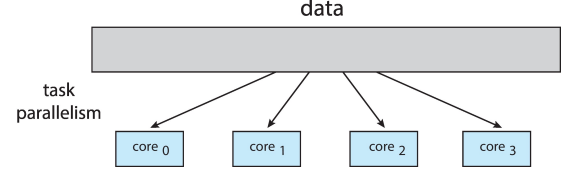
\includegraphics[width = 0.80\linewidth]{Images/48.png}
\end{center}
L'algoritmo di invio allora diventa: \newline
\begin{algorithm}[H]
\DontPrintSemicolon
\eIf{ack} {
    $M_{i+1}$
} {
    $M_i$ \tcp*[h]{è stato ricevuto un nack}
}
\end{algorithm}
\noindent
Un protocollo di questo tipo \textbf{funzionerebbe in una rete che introduce errori}. Sfortunatamente, le reti non solo introducono errori ma \textbf{anche perdite di pacchetti!}.
Prima di passare a definire un protocollo resistente anche alle perdite, parliamo di \textbf{efficienza di un protocollo}: quando si definisce un nuovo protocollo, si deve cercare di limitare
\textbf{il numero di messaggi diversi possibili in esso}, quindi se oltre a numerare i segmenti \textbf{numeriamo anche gli ack}
\begin{center}
    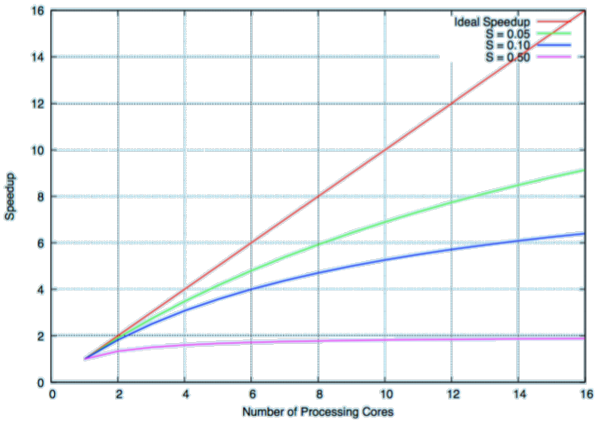
\includegraphics[width = 0.80\linewidth]{Images/49.png}
\end{center}
allora dovrò inserire una \textbf{regola aggiuntiva} che indica che, se non si è ricevuto il messaggio atteso, al posto di inviare un ack con numero di sequenza $i$ dovrò
inviare un ack con numero di sequenza $i-1$. L'algoritmo quindi diventa: \newline
\begin{algorithm}[H]
    \DontPrintSemicolon
    \eIf{ack} {
        $M_{i+1}$
    } {
        $M_i$ \tcp*[h]{è stato ricevuto un $ack_i$}
    }
    \end{algorithm}
\noindent
quindi, si andrà a ritrasmettere un messaggio se \textbf{si riceve un ack duplicato}.
Per rendere il protocollo resistente alle \textbf{perdite}: quando ho una perdita, può capitare che \textbf{il pacchetto inviato sia stato perso}
oppure che \textbf{l'ack vada perso}; allora viene introdotto \textbf{un timer}:
\begin{center}
    \includegraphics[width = 1\linewidth]{Images/50.png}
\end{center}
nel momento in cui \textbf{il timer scade} e non ho ancora ricevuto un ack, \textbf{rinvio lo stesso messaggio}. L'algoritmo di invio diventerà: \newline
\begin{algorithm}[H]
    \DontPrintSemicolon
    \eIf{$s+T$ is reached} {
        $M_i$\;
        set($s+T$) + $T$
    } {
        \eIf(\tcp*[h]{$s+T$ non è stato ancora raggiunto ($r$)}){$ack_i$} {
            $M_{i+1}$\;
            set($r+T$)
        } {
            $M_i$\;
            set($r+T$)
        }
    }
\end{algorithm}
\noindent
Questo tipo di implementazione è la più sofistica di quelli che vengono detti \textbf{protocolli stop-and-wait}.
Un protocollo stop-and-wait \textbf{funziona in una rete reale}. Tuttavia, vi sono delle problematiche:
\begin{itemize}
    \item L'impostazione della lunghezza del timer è un problema complesso
    \item Un timer \textbf{troppo corto} potrebbe causare \textbf{ritrasmissioni inutili}: nell'esempio fatto sopra, ci potrebbero essere lunghe sequenze di \textbf{ritrasmissioni inutili}
    \item Un timer \textbf{troppo lungo} ferma per troppo tempo la trasmissione in caso di perdita
\end{itemize}
\begin{center}
    \includegraphics[width = 0.25\linewidth]{Images/51.png}
\end{center}
Dovrò quindi avere un timer almeno lungo quanto il periodo di tempo che intercorre tra la trasmissione del messaggio e il ricevimento di un ack, questo valore
prende il nome di \textbf{Round-Trip Time} (RTT); il problema quindi passa al cercare di fare una stima accurata del RTT.
La problematica principale di un protocollo stop-and-wait è la seguente: supponiamo di essere nel caso in cui il \textbf{ritardo di trasmissione} non è più trascurabile
\begin{center}
    \includegraphics[width = 0.40\linewidth]{Images/52.png}
\end{center}
i parallelogrammi sopra rappresentano il ritardo di trasmissione, il quale vale $L/R$. Assumiamo, per semplicità, che gli ack
abbiano un ritardo di trasmissione trascurabile. Se siamo in un protocollo stop-and-wait, in questo caso esso è \textbf{altamente inefficiente}. Una
misura dell'efficienza del protocollo è la \textbf{utilità} (utility), la quale si calcola nel seguente modo:
$$U = \frac{\frac{L}{R}}{RTT + \frac{L}{R}}$$
questa misura indica \textbf{quanto tempo (da trasformare in percentuale) dedico effettivamente alla comunicazione}.
\subsubsection{Protocolli a finestra scorrevole}
\begin{center}
    \includegraphics[width = 0.30\linewidth]{Images/53.png}
\end{center}
Per risolvere il problema della \textbf{bassa utilità di stop-and-wait} sono stati pensati dei protocolli detti \textbf{a finestra scorrevole}
Questi protocolli permettono di trasferire fino a $W$ segmenti prima di \textbf{aspettare di ricevere gli ack dei vari segmenti inviati} (in questo caso si dice che la finestra si chiude).
Ciò significa che, una volta ricevuto l'ack del primo segmento \textbf{posso far scorrere la finestra e trasmettere il segmento $W$} e così via se non si hanno perdite. L'utilizzo del canale è quindi
molto più alto di stop-and-wait. La condizione per il quale c'è una condizione di \textbf{trasmissione continua} sul canale è che la finestra non si chiuda prima dell'arrivo del primo ack, cioè deve valere
la seguente condizione:
$$W \cdot \frac{L}{R} \geq RTT + \frac{L}{R}$$
invertendo la formula, posso quindi scoprire quanto deve essere grande la finestra per garantire una trasmissione continua:
$$W \geq \frac{RTT \cdot R}{L} + 1$$
C'è quindi da chiedersi \textbf{cosa deve essere ritrasmesso quando un segmento viene perso}.
Immaginiamo quindi di avere una finestra abbastanza ampia da non dover preoccuparci delle problematiche viste prima.
La prima possibilità è il protocollo \textbf{Go-Back-N}: la trasmissione va avanti e la finestra scorre \textbf{dopo ogni ack ricevuto}.
Se $s+T$ viene raggiunto, verranno ritrasmessi \textbf{tutti i segmenti a partire da quello che ha fatto scattare il timeout}
\begin{center}
    \includegraphics[width = 0.40\linewidth]{Images/54.png}
\end{center}
Il ricevitore, quando si accorge di aver ricevuto un segmento fuori sequenza, \textbf{scarta i segmenti fuori sequenza} e manda degli ack che "puntano" al primo segmento non ancora
ricevuto. Dal punto di vista del trasmettitore, appena inviato un segmento viene fatto partire un timer: se il timer scade, allora \textbf{ricomincerà a trasmettere tutti i segmenti a partire da quello per il quale il timer è scaduto}.
Tuttavia, questo protocollo non è particolarmente efficiente, perché \textbf{vado a scartare segmenti solo per poi riceverli di nuovo}, tuttavia questa implementazione \textbf{semplifica molto certi aspetti della trasmissione}: con questo protocollo
\textbf{non richiede buffer al destinatario}, poiché ogni segmento viene ricevuto in sequenza. Un'altra cosa importante di questo protocollo è il fatto che gli \textbf{ack sono comulativi}: per come è fatto il protocollo, i dati vengono
consegnati al livello applicativo \textbf{solo se sono in sequenza}; ciò significa che se io perdo un ack e successivamente l'ack per il segmento successivo \textbf{viene ricevuto correttamente}, allora posso essere sicuro che anche i segmenti successivi
siano stati trasmessi e ricevuti correttamente; cioè \textbf{gli ack dei segmenti successivi certificano la ricezione dei precedenti}. Ultimo dettaglio implementativo è che in questo protocollo \textbf{basta un solo timer per tutta la comunicazione}: viene fatto
ripartire dopo ogni ack ricevuto e si riferisce sempre al più vecchio segmento senza ack. \newline
Seconda possibilità è il protocollo \textbf{Selective Repeat}:
\begin{center}
    \includegraphics[width = 0.40\linewidth]{Images/55.png}
\end{center}
in questo protocollo, quando un segmento viene perso e il timer scatta per quel segmento, allora \textbf{viene ritrasmesso solo quel segmento} e non vengono
scartati gli altri segmenti. Chiaramente, in questo protocollo \textbf{ha la possibilità di avere segmenti fuori sequenza} e quindi ha bisogno di un buffer al
ricevitore per permettere il riordino dei segmenti prima di passarli al livello applicativo. Altra complicazione è che in questo protocollo gli ack sono \textbf{individuali}
e certificano solamente l'avvenuta ricezione di un segmento. Infine, \textbf{ogni segmento ha bisogno di un timer} per capire se esso è stato perso o meno.
Prima di continuare, facciamo un'osservazione: Go-Back-N e Selective repeat sono due esempi accademici l'uno opposto dell'altro. Nella realtà, si utilizzano \textbf{protocolli ibridi}
che utilizzano entrambi a seconda della situazione attuale della rete. TCP, infatti, è una soluzione ibrida tra questi due.
\subsection{Transmission Control Protocol (TCP)}
Transmission Control Protocol è un protocollo di trasporto \textbf{punto a punto}: vi è un singolo ricevitore e un singolo mittente che comunicano fra loro.
È un protocollo \textbf{affidabile}, che consegna i segmenti in ordine tramite uno \textbf{stream di byte}: in TCP quindi si fa riferimento ai \textbf{byte}, NON ai segmenti.
Non si hanno quindi \textbf{limiti del messaggio}, ciò che si va a fare è \textbf{contare i byte di dati all'interno del byte stream}; in ogni caso però i dati vengono inseriti nel
payload di un segmento e ogni singolo segmento può avere un payload di una certa dimensione massima, che prende il nome di \textbf{Maximum Segment Size} (MSS).
La comunicazione di TCP è \textbf{full-duplex}: vi è un flusso dati \textbf{bidirezionale} sulla stessa connessione.
TCP è \textbf{robusto a perdite di ack} e adotta il principio degli \textbf{ack comulativi}; inoltre è un protocollo \textbf{a finestra scorrevole}: per andare a impostare correttamente
la finestra d'invio utilizza due meccanismi di \textbf{controllo della congestione e di controllo del flusso}. È infine un protocollo \textbf{connection-oriented}, è quindi necessaria una fase
di "handshaking" (scambio di messaggi di controllo) in cui i due comunicanti si mettono d'accordo sui \textbf{parametri della connessione}.
La struttura di un segmento TCP è la seguente:
\begin{center}
    \includegraphics[width = 1\linewidth]{Images/56.png}
\end{center}
Alcune considerazioni:
\begin{itemize}
    \item Il bit $A$ viene settato ad 1 solamente se il messaggio è un \textbf{ack}: in TCP quindi ho solo messaggi o ack
    \item Le opzioni riguardano più ambiti (es. andare a negoziare la grandezza di MSS), quindi la grandezza di un header TCP è variabile e viene indicata dal campo \textit{header len}
    \item I bit $C$ ed $E$ servono ad indicare lo stato di congestione se si adotta la \textbf{congestione esplicita} e sono, in caso, impostati ad 1 dai router
    \item I bit $U$ e $P$ sono stati standardizzati e, se impostati ad 1, indicano che è necessario trasmettere \textbf{subito certi bit del pacchetto, considerati ad altra priorità}. Per come si è diffuso TCP, questi due bit non vengono quasi mai utilizzati
\end{itemize}
\subsubsection{Numeri di sequenza e di ACK}
Come vengono gestiti i \textbf{numeri di sequenza} e gli \textbf{ack} in TCP? Il numero di sequenza indica il \textbf{numero del byte stream del primo byte del segmento} mentre l'ack
indica il \textbf{numero di sequenza del prossimo byte che ci si aspetta di ricevere}. Vediamo quindi un esempio per fissare le idee:
\begin{center}
    \includegraphics[width = 0.80\linewidth]{Images/57.png}
\end{center}
\subsubsection{RTT in TCP e timeout}
Come viene impostato il timer di timeout in TCP? Questo aspetto è fondamentale per \textbf{evitare i problemi visti precedentemente} (trasmissioni inutili e tempi di risposta troppo alti)
Come facciamo però a stimare RTT? Nelle reti, il RTT varia molto e repentinamente tra segmenti di tipo diverso; dobbiamo quindi definire un meccanismo per cercare di impostare, in maniera approssimata,
un timer il più corretto possibile. Come fa TCP a stimare RTT?
\begin{itemize}
    \item Chiamiamo $SampleRTT$ il RTT che si misura dalla trasmissione al ricevimento dell'ack per un segmento specifico ignorando le ritrasmissioni.
    \item $SampleRTT$ cambia molto e in maniera repentina tra segmenti, vogliamo quindi \textbf{catturarne il trend}, non il $SampleRTT$ specifico: per impostare quindi il timer mi baserò su una misura meno netta, che chiamiamo $EstimatedRTT$, piuttosto che sul $SampleRTT$ del segmento precedente
\end{itemize}
Quindi come calcoliamo $EstimatedRTT$? Dobbiamo usare una tecnica che prende il nome di \textbf{Exponential Weighted Moving Average} (EWMA):
divido l'asse del tempo in \textbf{tempi discreti}, quindi l'$EstimatedRTT$ che deve essere calcolato al tempo $t$ è
$$EstimatedRTT[t] = (1-\alpha)\cdot EstimatedRTT[t-1] + \alpha \cdot SampleRTT[t]$$
\begin{center}
    \includegraphics[width = 0.65\linewidth]{Images/58.png}
\end{center}
L'influenza che i vari campioni sul valore di $EstimatedRTT$ decade esponenzialmente man mano che vado avanti nel tempo.
Un valore tipico di $\alpha$ è $\alpha = 0.125$. Per impostare l'intervallo di Timeout, dobbiamo però dobbiamo anche considerare
che le oscillazioni del RTT possono essere molto elevate, quindi impostiamo l'intervallo per il segmento che deve essere inviato al tempo $t$ nel seguente modo:
$$TimeoutInterval[t] = EstimatedRTT[t] + 4*DevRTT[t]$$
con l'ultimo addendo che rappresenta un "margine di sicurezza" per evitare i problemi legati ad una finestra impostata erroneamente.
$DevRTT[t]$ è la \textbf{deviazione}, calcolata tramite la tecnica EWMA, di $SampleRTT$ da $EstimatedRTT$ e si calcola nel seguente modo:
$$DevRTT[t] = (1-\beta)\cdot DevRTT[t-1] + \beta \cdot |SampleRTT[t] - EstimatedRTT[t]|$$
tipicamente, $\beta = 0.25$
\subsubsection{Trasmettiore TCP}
Ogni volta che si ricevono dati dallo strato applicativo, si effettuano le seguenti operazioni in un trasmettitore che usa TCP:\
\begin{itemize}
    \item Si crea un segmento con un numero di sequenza, il quale è definito come il primo byte del segmento all'interno del byte stream
    \item Viene fatto partire il \textbf{timer}: viene adottato un solo timer ed esso fa riferimento al più vecchio segmento per il quale non è stato ricevuto un ack. Viene impostato $TimeoutInterval$ utilizzano le formule viste sopra (per il primo pacchetto, $EstimatedRTT = SampleRTT$)
    \item Se \textbf{scatta il timeout}, ritrasmetto il segmento che lo ha causato e faccio ripartire il timer
    \item Una volta che viene ricevuto un ack, esso \textbf{risconta tutti i segmenti precedenti per i quali non sono ancora stati ricevuti degli ack}; si va ad aggiornare lo stato dei segmenti che prima si consideravano "in attesa di ack" e si fa ripartire il timer per i segmenti che non sono ancora stati riscontrati
\end{itemize}
\begin{center}
    \includegraphics[width = 0.75\linewidth]{Images/59.png}
\end{center}
\subsubsection{TCP fast retrasmit}
Il meccanismo \textbf{fast retransmit} fu introdotto dopo la pubblicazione delle specifiche di TCP. Esso fun introdotto per permettere di ritrasmettere in maniera rapida i segmenti persi
nel caso in cui la perdita di segmenti avvenga \textbf{in maniera sporadica} e non sia una condizione sistematica della rete.
\begin{center}
    \includegraphics[width = 0.85\linewidth]{Images/60.png}
\end{center}
Come funziona? Quando un segmento viene perso, \textbf{viene ritrasmesso dal ricevitore l'ack per l'ultimo segmento in ordine ricevuto}. Una volta che il trasmettitore riceve \textbf{3 ack duplicati} (senza contare il primo ack ricevuto, il quale riscontrava solamente la ricezione del segmento)
allora fast retransmit permette la \textbf{ritrasmissione del segmento con il più piccolo numero di sequenza non ancora riscontrato} anche se il timeout non è ancora scattato.
\subsubsection{TCP connection management e 3-way handshake}
\begin{center}
    \includegraphics[width = 0.95\linewidth]{Images/61.png}
\end{center}
Prima di iniziare a trasmettere, mittente e destinatario devono essere \textbf{d'accordo sullo stabilire una connessione e su quali parametri stabilire per essa}.
Infatti, alcuni parametri della connessione devono essere negoziati tra mittente e destinatario \textbf{prima} della trasmissione; questo viene effettuato attraverso 
\textbf{l'handshake}. TCP usa un \textbf{handshake a 3 vie}:
\begin{center}
    \includegraphics[width = 0.85\linewidth]{Images/62.png}
\end{center}
Le risorse vengono allocate \textbf{una volta ricevuto il messaggio di SYN} per il server e \textbf{una volta ricevuto il messaggio di SYNACK} per il client.
Già nell'ultimo messaggio, inoltre, potrei avere \textbf{un payload di dati}. TCP inoltre permette di chiudere la connessione tramite una negoziazione tra client e server:
\begin{center}
    \includegraphics[width = 0.85\linewidth]{Images/63.png}
\end{center}
Nel primo caso, il client vuole terminare la connessione, quindi il server \textbf{riscontra la volontà del client}, \textbf{termina l'invio dei dati restanti} e infine \textbf{chiude la connessione}.
Nel secondo caso, invece, il client vuole terminare la connessione e il server la chiude subito poiché \textbf{non ha ulteriori dati da inviare al client}. Notare che \textbf{anche un server può fare richiesta di terminazione di una connessione}.
\newpage
\subsubsection{TCP flow control}
\begin{center}
    \includegraphics[width = 0.65\linewidth]{Images/64.png}
\end{center}
Per mezzo del controllo di flusso, si permette che \textbf{il ricevitore possa controllare la quantità di dati che il mittente può inviare} per evitare di essere \textbf{sopraffatto e di portare i propri buffer al buffer overflow} (e quindi una perdita di segmenti).
Come si controlla a livello di trasporto il tasso di arrivo?
\begin{center}
    \includegraphics[width = 0.45\linewidth]{Images/65.png}
\end{center}
Il buffer ha una determinata dimensione $RcvBuffer$ e ad un certo istante di tempo, il buffer avrà una certa quantita di dati al suo interno
e una certa quantità di spazio libero, che chiamiamo $rwnd$. Il ricevitore quindi invia come feedback al mittente (immettendolo nell'header dell'ack nel campo \textit{receive window})
$rwnd$, in modo che il trasmettitore la quantità massima di dati che esso può accettare prima di andare in buffer overflow.
La finestra di trasmissione $W$ \textbf{viene quindi limitata in base al valore di receive window che esso riceve dal ricevente}.
\subsubsection{Principi del controllo di congestione}
Il controllo di congestione \textbf{riguarda la rete}: ci sono troppe sorgenti che inviano troppi dati troppo velocemente e quindi la rete non è in grado di gestirli.
In questo caso, si avranno \textbf{ritardi e possibili perdite di pacchetti}. È quindi \textbf{molto diverso dal controllo di flusso}.
Nel momento in cui la congestione cresce, \textbf{si ha una crescita dei pacchetti persi in rete}; se si adotta quindi un protocollo affidabile come TCP, si andrà ad \textbf{aumentare il numero di pacchetti ritrasmessi}.
L'aumento di ritrasmissioni quindi andrà a peggiorare la situazione. In questa situazione, si avrà \textbf{un aumento del throughput}, che andrà vicino al 100\% della capacità operativa della rete, tuttavia \textbf{si avrà una riduzione del "goodput"} (la quantità di dati ricevuti effettivamente utili all'applicazione)c
cala drasticamente
\begin{center}
    \includegraphics[width = 0.65\linewidth]{Images/66.png}
\end{center}
Vogliamo quindi tornare ad una situazione dove \textbf{throughput e goodput sono sovrapposti}. Un possibile approccio è il \textbf{controllo di congestione end-to-end}:
\begin{center}
    \includegraphics[width = 0.65\linewidth]{Images/67.png}
\end{center}
in questo tipo di controllo di congestione, la rete non dà \textbf{nessun feedback esplicito} e lo stato della rete viene \textbf{inferito in base alle perdite e dai ritardi dei segmenti e degli ack che vengono ricevuti dai sistemi host}.
Questo tipo di approccio è quello adottato da TCP.
Un altro approccio, non frequentemente adottato, è quello del \textbf{controllo di congestione network-assisted}: in questo tipo di controllo di congestione,
i \textbf{router} hanno la capacità di fornire informazioni puntuali riguardante il loro \textbf{stato di congestione} (si può fare utilizzando i bit $C$ ed $E$ dell'header TCP).
\begin{center}
    \includegraphics[width = 0.65\linewidth]{Images/68.png}
\end{center}
\subsubsection{TCP congestion control}
L'approccio di TCP al controllo di congestione si dice del tipo \textbf{Additive Increase Multiplicative Decrease}: si parte da un tasso di invio dei byte
molto basso che \textbf{incrementerò gradualmente} (additive increase); prima o poi, avverrà una perdita poiché il \textbf{tasso di invio è diventato troppo elevato}, in questo caso
vado a \textbf{dimezzare il tasso di invio per evitare che ci siano altre perdite}:
\begin{center}
    \includegraphics[width = 0.85\linewidth]{Images/69.png}
\end{center}
Vediamo quindi le fasi di questo meccanismo:
\begin{enumerate}
    \item \textbf{Slow start}: il numero di segmenti trasmessi (MSS) ad ogni RTT viene limitato dalla \textbf{finestra di congestione} $cwnd$.
    Quando la connessione inizia, viene \textbf{fatto incrementare esponenzialmente} il tasso di invio fino alla prima perdita di un pacchetto:
    \begin{itemize}
        \item Inizialmente, $cwnd = 1$
        \item $cwnd$ viene \textbf{raddoppiata} ad ogni RTT; ciò viene fatto \textbf{incrementando RTT ad ogni ack ricevuto}
    \end{itemize}
    In breve, \textbf{si ha un inizio lento, tuttavia il tasso di invio aumenta esponenzialmente}
    \begin{center}
        \includegraphics[width = 0.35\linewidth]{Images/70.png}
    \end{center}
    \item \textbf{Congestion avoidance}: Quando la crescita da esponenziale deve diventare lineare? TCP indica che ciò deve avvenire quando \textbf{$cwnd$ arriva a metà del suo valore prima dell'ultimo timeout sperimentato}. Questo meccanismo
    si può implementare attraverso una variabile che prende il nome di $sstresh$ che, quando si verifica un evento di perdita, viene posta a \textbf{metà del valore che aveva $cwnd$ prima dell'evento di perdita}
    \begin{center}
        \includegraphics[width = 0.65\linewidth]{Images/71.png}
    \end{center}
    La primissima implementazione di TCP (\textbf{TCP tahoe}), poneva immediatamente $cwnd$ ad 1 in caso di evento di perdita.
    Una versione più recente di TCP detta \textbf{TCP Reno} adotta invece il meccanismo di \textbf{Fast Recovery}: se l'evento di perdita è stato causato da \textbf{3 ack duplicati} invece che da un evento di \textbf{timeout},
    invece di andare ad impostare $cwnd$ ad 1, essa viene impostata a $cwnd = sshtresh + 3 \cdot MSS$; in caso di timeout, invece, rimane il comportamento di TCP Tahoe
\end{enumerate}
La trasmissione in TCP viene quindi dominata \textbf{o dalla finestra di congestione ($cwnd$) o dalla finestra di ricezione ($rwnd$)}, cioè se domina il controllo di flusso oppure il controllo di congestione
\begin{center}
    \includegraphics[width = 0.55\linewidth]{Images/72.png}
\end{center}
Quindi la finestra di trasmissione è posta a $min\{cwnd, rwnd\}$ bytes; dopodiché si aspetta un RTT per gli ack e infine si inviano altri byte.
Quando $cwnd < rwnd$, il controllo di congestione è dominante rispetto al controllo di flusso.
Il trasmettitore TCP quindi andrà a limitare la propria trasmissione, quindi deve valere che
$$LastByteSent - LastByteAcked \leq min\{cwnd, rwnd\}$$
$cwnd$ è \textbf{dinamicamente aggiustata} in base alle condizioni di rete osservate (implementando il controllo di congestione TCP).
$rwnd$ è invece aggiustato basandosi \textbf{sul valore ricevuto dal ricevente} (implementando il controllo di flusso TCP).
\section{Livello di rete: Piano dati}
\begin{center}
    \includegraphics[width = 0.75\linewidth]{Images/73.png}
\end{center}
L'obbiettivo del livello di rete è trasportare i segmenti provenienti dal livello di trasporto dal \textbf{mittente} al \textbf{ricevente}.
\begin{itemize}
    \item \textbf{Mittente}: incapsula i segmenti in \textbf{datagrammi} che passerà al livello di collegamento
    \item \textbf{Ricevente}: Decapsula i segmenti dai datagrammi e li consegna al livello di trasporto
\end{itemize}
I protocolli del livello di rete sono presenti in \textbf{tutti i dispositivi capaci di connettersi ad internet}, cioè sono presenti sia negli host che nei router.
In particolare, i \textbf{router}:
\begin{itemize}
    \item Esaminano campi dell'intestazione dei datagrammi che passano attraverso di loro
    \item Muovono i datagrammi dalle porte di input alle porte di output corretta, in modo da trasferire i datagrammi lungo un cammino punto a punto (end-to-end) corretto tra il mittente e il destinatario
\end{itemize}
Due funzionalità chiave del livello di rete sono:
\begin{itemize}
    \item \textbf{Inoltro (forwarding)}: Muove i pacchetti dal collegamento in input del router all'appropriato collegamento in uscita dello stesso
    \item \textbf{Instradamento (routing)}: Determina la strada che un pacchetto deve intraprendere per raggiungere, dalla sorgente, la propria destinazione. Questo processo viene effettuato attraverso \textbf{algoritmi e protocolli di routing}
\end{itemize}
Il livello di rete è suddiviso in \textbf{due diversi "piani"}:
\begin{itemize}
    \item \textbf{Piano dati (Data plane)}: Ha valenza \textbf{locale} e riguarda le funzioni che vengono eseguite dai singoli router della rete per determinare l'interfaccia corretta verso quale inviare il pacchetto. Determina quindi COME un datagramma che arriva alle porte di input di un router debba essere inoltrato alle sue porte in uscita. Il piano dei dati, quindi, implementa \textbf{l'inoltro}.
    \item \textbf{Piano di controllo (Control plane)}: Ha valenza \textbf{su tutta la rete} (network-wide). Determina come un datagramma debba essere instradato tra i router, lungo un percorso end-to-end, dall'host sorgente all'host destinazione. Il piano di controllo, quindi, \textbf{implementa l'instradamento}.
    In realtà, il piano di controllo, nella sua accezione più generale possibile, non implementa solamente l'instradamento ma anche tutti i protocolli e tutti gli algoritmi \textbf{necessari a far funzionare la rete}. Esistono due differenti approcci di implementazione del piano di controllo:
    \begin{itemize}
        \item \textbf{Algoritmi di instradamento tradizionali}: Approccio distribuito, in cui il piano di controllo della rete (o una sua parte) viene implementato su ogni singolo dispositivo di rete. Ogni singolo router quindi \textbf{implementa il piano di controllo} 
        \item \textbf{Software Defined Networking (SDN)}: Il piano di controllo viene \textbf{centralizzato e implementato su server remoti} (anche in cloud). Si ha quindi un \textbf{controllore centralizzato} che ha una \textbf{visione globale} della rete e che prenderà le decisioni riguardanti l'instradamento dei pacchetti.
    \end{itemize}
    Questi appunti tratteranno solamente il primo approccio.
\end{itemize}
Nell'approccio tradizionale, ogni singolo router \textbf{ha un piano di controllo in cui vengono eseguiti gli algoritmi di routing}; si ha quindi uno \textbf{scambio di messaggi tra i vari router} per fare in modo di \textbf{popolare correttamente le proprie tabelle di inoltro}.
\begin{center}
    \includegraphics[width = 0.80\linewidth]{Images/74.png}
\end{center}
Nell'approccio SDN, il piano di controllo viene \textbf{centralizzato in dei server}, i quali eseguono il controllore remoto; il quale si
interfaccerà con i dati provenienti da ogni singolo router per \textbf{ottenere informazioni sulla rete} (es. informazioni topologiche), ottenendo
così una \textbf{visione del piano dei dati}. Conoscendo quindi tutte le informazioni necessarie su tutti i router della rete, il controller può prendere
decisioni riguardanti l'instradamento dei pacchetti, cioè \textbf{genererà le tabelle di inoltro}, le quali verranno inviate ai singoli router per poter effettuare le operazioni di inoltro.
\begin{center}
    \includegraphics[width = 0.80\linewidth]{Images/75.png}
\end{center}
\subsection{Modello di servizio dello strato di rete}
Qual è il modello di servizio che viene adottato per trasportare, a livello di rete, i datagrammi dalla sorgente al destinatario?
Per esempio, ci potrebbero essere varie tipologie di servizi che potrebbero essere offerti a... 
\begin{itemize}
    \item \textbf{Singoli datagrammi}: garanzia di consegna, garanzia di consegna con un ritardo massimo di 40ms ecc...
    \item \textbf{Flussi di datagrammi}: Garanzia di consegna in ordine, larghezza di banda minima ecc...
\end{itemize}
Tuttavia, a livello di rete, il modello di servizio adottato è di tipo \textbf{"best effort"}, quindi \textbf{non vi sono}:
\begin{itemize}
    \item Garanzie sulla consegna dei datagrammi al ricevente
    \item Garanzie sull'ordine di consegna
    \item Garanzie sulla larghezza di banda disponibile per il flusso lungo il percorso end-to-end
\end{itemize}
\begin{center}
    \includegraphics[width = 0.80\linewidth]{Images/76.png}
\end{center}
\subsection{Architettura di un router}
L'architettura generica di un router può essere visualizzata nel seguente modo:
essa prevede l'esistenza \textbf{di un certo numero di porte (o interfacce) in ingresso} e di un certo numero di \textbf{porte (o interfacce) in uscita}.
In realtà, ogni singola porta di un router può agire \textbf{sia come porta di ingresso, sia come porta di uscita}, tuttavia, a livello funzionale, è necessario
mantenere una distinzione fra le due. Tra le porte di ingresso e le porte in uscita si trova una \textbf{maglia di commutazione ad alta velocità} (high-speed switching fabric), il quale è una
\textbf{rete fisica}, solitamente implementata con circuiti integrati, che mette in comunicazione \textbf{ogni singola interfaccia di ingresso con ogni singola interfaccia in uscita}.
La switching fabric, tuttavia, \textbf{non ha un collegamento da ogni singola porta in ingresso ad ogni singola porta in uscita} (full mesh), poiché ciò risulterebbe in una complessità \textbf{molto elevata};
invece, l'implementazione di questa rete segue delle teorie che \textbf{permettono di andare a definire delle "reti di commutazione" all'interno della maglia}, le quali permettono di mettere in comunicazione le porte di ingresso con le porte di uscita
\textbf{mantenendo limitato il numero di collegamenti complessivi}.
Le reti di commutazione devono garantire \textbf{la possibilità di inviare pacchetti da un'interfaccia in ingresso ad un'interfaccia in uscita indipendentemente da ciò che sta accadendo sulle altre interfacce}.
Se una rete ha questa proprietà si dice che essa è \textbf{non bloccante}.
Il componente che permette l'esecuzione di tutte le operazioni di routing è il \textbf{processo di routing} (routing processor), il quale si trova nel \textbf{piano di controllo} del livello di rete.
\begin{center}
    \includegraphics[width = 0.80\linewidth]{Images/77.png}
\end{center}
Dall'immagine sopra, possiamo notare che \textbf{il piano dei dati e il piano di controllo operano su ordini di tempo molto diversi tra di loro}:
\begin{itemize}
    \item A livello di piano dati, viene effettuato lo \textbf{spostamento dei pacchetti dalle interfacce di ingresso a quelle di uscita}. Questa operazione deve essere effettuata \textbf{il più velocemente possibile}, vista anche la grande mole di pacchetti
    che si possono avere in un singolo router. L'ordine di tempo quindi, in questo contesto, è nell'ordine dei \textbf{nanosecondi}
    \item Le decisioni prese a livello di controllo, invece, possono anche essere applicate alla rete in un tempo nell'ordine dei \textbf{millisecondi}
\end{itemize}
Le \textbf{porte in ingresso} di un router hanno la seguente architettura:
\begin{center}
    \includegraphics[width = 1\linewidth]{Images/78.png}
\end{center}
analizziamola nel dettaglio
\begin{itemize}
    \item \textbf{Terminazione di linea} (line termination): È l'interfaccia verso il mondo esterno (es. porta Ethernet); si occupa di \textbf{ricevere i bit in ingresso}. Le funzionalità della terminazione di linea sono quindi
    relative al \textbf{livello fisico}
    \item \textbf{Protocollo del livello di collegamento}: Una volta ricevuti i bit del pacchetto, essi vengono passati al \textbf{livello di collegamento}, dove viene effettuato un protocollo a livello di collegamento per organizzare i bit in una \textbf{trama} (frame) e decapsulare il pacchetto in un \textbf{datagramma}
    \item \textbf{Lookup e inoltro}: Si utilizzano le informazioni contenute nei campi dell'intestazione del datagramma (ricevuto dallo strato precedente) per \textbf{interrogare la tabella di inoltro memorizzata nella memoria dell'interfaccia di input} (lookup) allo scopo di \textbf{trovare una corrispondenza} (match). 
    L'inoltro del pacchetto verso una porta di output avviene quindi in base alla corrispondenza trovata. Questa serie di azioni vengono dette \textbf{"match plus action"}.
    Quali sono però i campi dell'intestazione del datagramma che vengono utilizzati per prendere decisioni a livello di inoltro?
    Nel caso specifico di internet, viene utilizzato un approccio \textbf{basato sull'indirizzo IP di destinazione} (destination-based forwarding) contenuto nell'intestazione del datagramma;
    tuttavia, esistono anche altri tipi di meccanismi (es. \textbf{source-based forwarding}, dove viene preso in considerazione anche l'indirizzo IP sorgente).
\end{itemize}
Ogni singola porta in ingresso presenta \textbf{una coda}; ciò significa che si può avere una \textbf{situazione di accodamento nelle porte di ingresso di un router} quando il tasso di arrivo dei pacchetti è maggiore rispetto alla velocità con la quale lo switching fabric è in grado di smaltirli verso le porte in uscita.
La velocità di inoltro della switching fabric dei pacchetti sulle porte di ingresso verso le interfacce di output prende il nome di \textbf{switching rate}:
\begin{itemize}
    \item Viene spesso misurato come \textbf{multiplo del tasso di linea (line rate) $R$ della porta di input/output}, cioè della \textbf{velocità della porta}
    \item Se si hanno $N$ porte di ingresso/uscita (il numero coincide poiché ogni porta di input può diventare una porta di output e viceversa), allora è desiderabile uno switching rate di almeno $N \cdot R$, poiché esso garantisce un accodamento nelle porte di ingresso \textbf{trascurabile}.
\end{itemize}
\begin{center}
    \includegraphics[width = 0.70\linewidth]{Images/79.png}
\end{center}
Perché questo è fondamentale? Se si è nella condizione in cui lo switching rate è più basso di $N \cdot R$ (tasso di linea di tutte le porte di ingresso), allora si potrebbe avere 
\textbf{un accodamento molto elevato nelle porte di ingresso} e quindi avere delle perdite dovute ad un buffer overflow. In più, un ulteriore problema generato da un accodamento significativo nelle porte
di ingresso è il problema del \textbf{Head-of-the-line (HOL) blocking}: i datagrammi che si sono accodati nelle porte di ingresso del router \textbf{vengono bloccati dai datagrammi che si trovano davanti a loro nella coda}, i quali, al momento, non possono essere trasmessi verso la porta di output corretta.
Perché si può verificare questo fenomeno?Se si hanno due pacchetti, \textbf{provenienti da interfacce in ingresso differenti}, che devono essere inoltrati \textbf{verso la stessa porta in uscita}, allora questo
trasferimento non può avvenire in contemporanea per entrambi i pacchetti. Infatti, se provassi a trasmettere i due pacchetti insieme, essi finirebbero per \textbf{mischiarsi} (si avrebbe quindi una \textbf{collisione}) e quindi diventerebbero entrambi \textbf{inintelligibili}.
Quindi, uno dei due pacchetti dovrà \textbf{aspettare che la trasmissione dell'altro pacchetto si concluda} prima di essere trasmesso. 
\begin{center}
    \includegraphics[width = 0.901\linewidth]{Images/80.png}
\end{center}
Il problema dell'HOL-Blocking può \textbf{provocare la crescita indefinita del tempo di accodamento}; ragione per il quale è assolutamente necessario dimensionare lo switching fabric in maniera opportuna. \newline
Una \textbf{porta di output} di un router è invece strutturata come segue:
\begin{center}
    \includegraphics[width = 0.901\linewidth]{Images/81.png}
\end{center}
La struttura è pressoché identica a quella di una porta di ingresso; ovviamente, le operazioni effettuate all'interno della porta di uscita sono quelle di \textbf{incapsulamento del datagramma in una trama del livello di collegamento} e la
trasmissione in uscita del pacchetto. Anche in questo caso, le porta di output presentano un \textbf{buffer}, nei quali i pacchetti si accoderanno ogni qual volta il tasso di arrivo dei pacchetti dello switching fabric è più elevato del tasso di trasmissione
delle porte. Si potrebbero quindi avere, anche in questo caso, ritardi di accodamento e buffer overflow. \textbf{L'accodamento nelle porte di output è un problema fisiologico dei router} ed è quindi non eliminabile; tutta la trattazione dei ritardi di accodamento
vista fino ad ora era quindi riferita \textbf{ad un accodamento nelle porte di output, assumendo un accodamento in input trascurabile}.
Poiché l'accodamento nelle porte di output non è eliminabile, si rende necessario \textbf{capire come gestire e trasmettere in uscita i pacchetti si accodano nel buffer}.
In generale, \textbf{non è vero che, in generale, il primo pacchetto che arriva è il primo pacchetto che viene trasmesso} (politica FIFO); in realtà, i pacchetti possono avere \textbf{priorità di tipo differente}, quindi 
si rendono necessaire delle politiche che \textbf{regolino sia lo scarto preventivo dei pacchetti} sia \textbf{quali pacchetti verranno scelti per essere trasmessi in uscita}:
\begin{itemize}
    \item \textbf{Drop policy}: Al posto di far riempire la coda fino al punto di riempirla, quindi arrivare ad una situazione in cui ogni pacchetto successivo viene scartato per buffer overflow, tendenzialmente si tende a \textbf{scartare preventivamente dei pacchetti} quando il livello di occupazione della coda raggiunge una certa soglia.
    Tendenzialmente vengono scartati i pacchetti a più bassa priorità.
    \item \textbf{Discipline di scheduling}: Una volta che si hanno dei pacchetti accodati, quali sono quelli che \textbf{verranno trasmessi per primi?} Esistono delle politiche diverse (es. \textbf{Priority scheduling}: chi ha la più alta priorità).  
\end{itemize}
\subsection{Internet Protocol (IP)}
Il \textbf{protocollo IP} è un protocollo dello strato di rete che si occupa dell'indirizzamento dell'instradamento dei pacchetto; esso è \textbf{fondamentale per il funzionamento della rete internet}.
Il datagramma del protocollo IP ha la seguente struttura:
\begin{center}
    \includegraphics[width = 1\linewidth]{Images/82.png}
\end{center}
Vediamoli più in dettaglio:
\begin{itemize}
    \item \textbf{Version}: Ha lunghezza di 4 bit e riguarda la versione del protocollo utilizzata (es. IPv4, IPv6 [quest'ultimo, non oggetto del corso])
    \item \textbf{Header length}: Ha lunghezza di 4 bit e riporta la \textbf{lunghezza dell'header in byte}. Questo campo si rende necessario poiché il protocollo IP \textbf{prevede la presenza di eventuali opzioni}, le quali possono allungare la dimensione dell'intestazione.
    \item \textbf{Length}: Ha lunghezza di 16 bit e riporta la \textbf{lunghezza totale del datagramma in byte}. Ovviamente $\textrm{Length} - \textrm{Header length} = \textrm{Payload length}$. Poiché si hanno 16 bit per codificare la lunghezza del datagramma, allora la sua massima dimensione possibile
    sarà $2^{16} - 1 \approx 65.000$ byte; solitamente, però, la lunghezza di un datagramma IP è di $1500$ byte perché si tende a dimensionare un pacchetto in modo tale che sia \textbf{al più grande quanto la massima lunghezza supportata da una trama a livello di collegamento}.
    \item \textbf{Type of service}: Ha lunghezza 8 bit ed indica la \textbf{priorità del pacchetto}
    \item \textbf{Time to live (TTL)}: Ha lunghezza 8 bit e non è altro che un \textbf{contatore} che viene decrementato da ogni router che il pacchetto attraversa. Il massimo del TTL è $2^8 - 1 = 255$.
    Questo campo è necessario per evitare che un pacchetto mal indirizzato o finito in un loop della rete \textbf{rimanga per sempre presente al suo interno}.
    \item \textbf{Upper layer}: Ha lunghezza 8 bit e indicano quale \textbf{protocollo di trasporto sta venendo utilizzato per il payload di questo pacchetto}; questo campo serve per \textbf{effettuare le operazioni di multiplazione e demultiplazione a livello di rete}.
    \item \textbf{Fragmentation reassembly}: Questi 3 campi, rispettivamente di 16, 4 e 12 bit, venivano utilizzati per la \textbf{frammentazione}. IP prevede che, nel caso il datagramma sia di dimensioni maggiori rispetto alla massima dimensione gestita dal protocollo di collegamento, esso possa essere \textbf{frammentato in pacchetti di dimensioni più piccole}, che poi alla destinazione verranno \textbf{ricombinati nel datagramma originario}.
    Di fatto, la frammentazione non avviene quasi mai nelle reti moderne. La frammentazione di un datagramma introduce diversi problemi, come \textbf{la necessità di dover avere un buffer al destinatario} o il \textbf{dover ricostruire un datagramma da dei pacchetti arrivati fuori sequenza}.
    \item \textbf{Header checksum}: Ha lunghezza 16 bit e viene usato per \textbf{effettuare un controllo su eventuali errori sul solo header IP (NON SUL PAYLOAD)}.
    \item \textbf{Source IP address}: Ha lunghezza 32 bit e indica l'indirizzo IP di chi ha generato il datagramma
    \item \textbf{Destination IP address}: Ha lunghezza 32 bit e indica l'indirizzo IP di destinazione del datagramma
    \item \textbf{Options}: Questo campo ha lunghezza 32 bit e indica diverse opzioni del protocollo IP che possono essere attivate per la trasmissione (es. Registrare il percorso effettuato)
\end{itemize}

\subsubsection{Indirizzamento IP}
Come vengono \textbf{assegnati gli indirizzi IP?}
L'indirizzo IP è un identificatore di 32 bit (come visto nell'intestazione dell'header IP) associato \textbf{ad ogni interfaccia di un host/router}.
L'indirizzo IP non è quindi \textbf{proprio dell'host/router ma delle sue interfacce}. Un host, tuttavia, potrebbe avere diverse interfacce (es. WiFi ed Ethernet);
quindi ad ognuna di esse si \textbf{assegna un indirizzo IP differente}. Questa situazione "peggiora" nei router (ogni router ha almeno 3 interfacce, altrimenti non avrebbe senso avere un router), in quanto \textbf{ad ogni loro interfaccia viene assegnato un indirizzo IP differente}.
Ricordiamo che, in questo contesto, \textbf{i termini "porta" ed "interfaccia" sono sinonimi}. 
\begin{center}
    \includegraphics[width = 0.60\linewidth]{Images/83.png}
\end{center}
\begin{center}
    \includegraphics[width =1\linewidth]{Images/84.png}
\end{center}
L'indirizzo IP è solitamente rappresentato in \textbf{notazione decimale puntata}; cioè si raggruppano i 32 bit in 4 gruppi da 8 bit, si converte ogni gruppo in
in decimale e si separano i 4 numeri ottenuti con un punto.
Arrivati a questo punto, dobbiamo quindi chiederci \textbf{come le varie interfacce sono effettivamente collegate fra di loro}.
Tuttavia, questo argomento appartiene al \textbf{livello di collegamento}; per il momento, l'unica cosa che dobbiamo sapere è che gli host (o le interfacce dei router) che
\textbf{che non hanno, a loro volta, nel mezzo un router possono essere tutte raggiungibili l'una dall'altra}. Tutte le interfacce che sono raggiungibili direttamente tra di loro \textbf{senza passare da un router}
fanno parte della stessa \textbf{sottorete}; il termine sottorete è di fatto \textbf{equivalente al termine "rete" fino ad ora presentato}.
Gli indirizzi IP sono strutturati in modo tale che \textbf{tutte le interfacce (router o host) che appartengono alla stessa sottorete avranno i bit più significativi identici}.
Quindi, l'indirizzo IP è strutturato in una parte, relativa ai bit più significativi dell'indirizzo, \textbf{chiamata "parte di sottorete" (o prefisso)} e una parte, relativa ai bit restanti, prende il nome di \textbf{"parte di host"}.
Tutte le interfacce appartenenti alla stessa sottorete avranno quindi la parte di sottorete del loro indirizzo IP identiche, mentre avranno parte di host diverse.
Come facciamo però a \textbf{definire una sottorete?}
Per farlo, "stacchiamo" ogni interfaccia dal suo host o router, creando quindi "isole" di reti isolate.
Ogni rete isolata è quindi una \textbf{sottorete}; la quale ha \textbf{un suo indirizzo IP, che prende il nome di "indirizzo di sottorete"}, il quale \textbf{identifica univocamente la sottorete}.
Facciamo un esempio: supponiamo di avere il seguente indirizzo di sottorete:
\begin{center}
    233.1.1.0/24
\end{center}
Cosa significa "/24"? L'indirizzo di sottorete è quell'indirizzo \textbf{ottenuto mettendo tutti i bit relativi alla parte di host a 0}; il "/24" indicano quanti bit appartenenti alla parte di sottorete
appartengono, partendo dal bit più significativo, alla "parte di sottorete" dell'indirizzo.
Per definire le sottoreti, vi sono due approcci:
\begin{itemize}
    \item \textbf{Classless InterDomain Routing}: In questo approccio, si ha piena flessibilità sul numero dei bit che si possono assegnare alla parte di sottorete e alla parte di host dell'indirizzo.
    Il formato dell'indirizzo è quindi "a.b.c.d/x" dove $x$ è il numero di bit nella parte di sottorete dell'indirizzo. Una rappresentazione alternativa dello "/" è la \textbf{maschera di sottorete} (subnet mask),
    la quale non è altro che un indirizzo dove si impostano \textbf{tutti a 1 i bit relativi alla parte di sottorete e tutti a 0 i bit relativi alla parte di host}. Nei router, di solito viene utilizzata, per ragioni implementative,
    la rappresentazione con maschera di sottorete.
    \begin{center}
        \includegraphics[width =0.80\linewidth]{Images/85.png}
    \end{center}
    \item \textbf{Classfull IP Addressing}: Storicamente, l'approccio utilizzato per definire le sottoreti divide gli indirizzi in \textbf{3 classi diverse}:
    \begin{itemize}
        \item \textbf{Classe A}: Questi indirizzi hanno il primo bit più significativo impostato a 0; essi hanno \textbf{8 bit per la parte di sottorete e i restanti per la parte di host}
        \item \textbf{Classe B}: Questi indirizzi hanno i primi due bit più significativi impostati rispettivamente a 1 e 0; essi hanno \textbf{16 bit per la parte di sottorete e i restanti per la parte di host}
        \item \textbf{Classe C}: Questi indirizzi hanno i primi tre bit più significativi impostati rispettivamente a 1, 1, e 0; essi hanno \textbf{24 bit per la parte di sottorete e i restanti per la parte di host}
    \end{itemize}
    \begin{center}
        \includegraphics[width =0.80\linewidth]{Images/86.png}
    \end{center}
    Questo tipo di indirizzamento \textbf{non richiede l'esistenza della maschera di sottorete}; infatti, si può identificare quanti bit sono dedicati alla parte di sottorete e alla parte di host semplicemente osservando il valore dei primi bit dell'indirizzo.
    Tuttavia, questo tipo di indirizzamento \textbf{non viene più utilizzato}, poiché è troppo rigido
\end{itemize}
\subsubsection{Indirizzi IP speciali}
\begin{center}
    \includegraphics[width =0.50\linewidth]{Images/87.png}
\end{center}
Gli indirizzi IP speciali sono \textbf{indirizzi IP che non possono essere assegnati agli host}; essi sono i seguenti:
\begin{itemize}
    \item \textbf{Indirizzo di sottorete}: Indirizzo IP con la parte di host impostata con tutti i bit a 0.
    \item \textbf{Direct Broadcast Address}: Indirizzo IP con la parte di host impostata con tutti i bit a 1. Questo tipi di indirizzo permette di inviare un pacchetto \textbf{dall'esterno verso tutti gli host di una sottorete}.
    Di fatto, questo tipo di indirizzi non viene mai utilizzato, poiché viene scartato a priori dai router.
    \item \textbf{Limited Broadcast Address}: Indirizzo IP con tutti i bit impostati a 1. Questo indirizzo permette di inviare un pacchetto a \textbf{tutti gli host all'interno della sottorete in cui viene generato}; tuttavia, questo pacchetto non potrà superare i router, poiché verrà scartato da essi.
\end{itemize}
\subsection{Destination-based forwarding}
Una tabella di inoltro, in generale, ha la seguente struttura:
\begin{center}
    \includegraphics[width =0.90\linewidth]{Images/88.png}
\end{center}
quindi, per ognuna delle sue righe, non viene specificato un singolo indirizzo IP ma invece un \textbf{intervallo di indirizzi IP}; più nello specifico, in ogni riga della
tabella di inoltro viene specificato \textbf{l'indirizzo IP di sottorete, accompagnato dalla sua subnet mask}. Viene inoltre specificata, per ogni riga, \textbf{l'interfaccia verso la quale inviare il pacchetto in caso si abbia un match}.
Di fatto, questo è un modo compatto per rappresentare \textbf{l'indirizzo IP di sottorete più la sua subnet mask}.
Solitamente, in una tabella di inoltro è presente anche una riga che prende il nome di \textbf{default route}, la quale sarà la riga con cui il pacchetto ha un match \textbf{se esso non ha avuto un match con nessuna delle altre righe della tabella}.
Nel caso in cui l'indirizzo di destinazione di un pacchetto \textbf{abbia più di un solo match con gli indirizzi all'interno della tabella}, si segue il principio del \textbf{longest prefix match}: Quando si effettua la ricerca, per un dato indirizzo IP, di una
voce all'interno della tabella di inoltro, \textbf{utilizza la voce che corrisponde all'indirizzo di destinazione che presenta il prefisso più lungo}; cioè che corrisponde all'indirizzo IP di destinazione per un numero maggiore di bit.
\subsection{Dynamic Host Configuration Protocol (DHCP)}
Fino ad ora, abbiamo parlato di come inoltrare un datagramma IP e come definire una sottorete tramite un indirizzo IP.
Tuttavia, \textbf{come si fa ad ottenere un indirizzo IP?} In realtà, questa domanda ne contiene altre due:
\begin{enumerate}
    \item Come fa un host ad ottenere un indirizzo IP all'interno della sua rete? (Parte dell'host dell'indirizzo)
    \item Come fa una rete ad ottenere un indirizzo IP per se stessa? (Parte di sottorete dell'indirizzo)
\end{enumerate}
Rispondiamo alla \textbf{prima domanda}: ci sono fondamentalmente due modi per un host di ottenere un indirizzo IP:
\begin{itemize}
    \item Specificandolo staticamente in un file di configurazione del sistema operativo (es. /etc/rc.config in UNIX)
    \item \textbf{DHCP}: Ottiene dinamicamente un indirizzo da un server, chiamato \textbf{DHCP server}. Questa architettura è di tipi "client-server" ed è trasparente all'utente
\end{itemize}
L'obbiettivo di DHCP è quello di far ottenere agli host un indirizzo IP \textbf{quando essi si "uniscono" alla rete}
\begin{itemize}
    \item L'host ottiene \textbf{un indirizzo IP temporaneo per un determinato "lease time" (tempo di prestito)}; una volta che il lease time scade, l'indirizzo IP viene \textbf{deallocato per l'utente}.
    Gli host possono rinnovare \textbf{il "prestito" dell'indirizzo IP}
    \item \textbf{Permette il riuso di indirizzi} (un indirizzo IP viene mantenuto solamente quando un host che lo utilizza è connesso)
\end{itemize}
Il protocollo DHCP prevede lo scambio di quattro messaggi:
\begin{itemize}
    \item L'host manda il messaggio \textbf{DHCP discover} in broadcast (tramite l'indirizzo IP di broadcast limitato) (opzionale)
    \item Il server DHCP risponde con un messaggio \textbf{DHCP offer} in broadcast (opzionale)
    \begin{itemize}
        \item I due step sopra possono essere evitati \textbf{se il client "ricorda" un indirizzo IP che gli è stato assegnato precedentemente dal server DHCP} (RFC 2131)
    \end{itemize}
    \item L'host richiede un indirizzo IP (messaggio \textbf{DHCP request})
    \item Il server DHCP \textbf{invia l'indirizzo da utilizzare all'host} (messaggio \textbf{DHCP ack})
\end{itemize} 
Tipicamente, il DHCP server è \textbf{co-localizzato nel router}, in modo che possa servire le sottoreti a cui il router è collegato.
DHCP si basa \textbf{sul protocollo UDP} sulle porte note \textbf{68 e 67}, rispettivamente la porta su cui si mettono in ascolto i \textbf{client DHCP} e \textbf{i server DHCP}.
All'inizio della comunicazione, il client definisce un \textbf{transaction ID}, il quale verrà riportato nelle risposte del server DHCP. Il transaction ID è necessario per il client
per \textbf{riconoscere i messaggi destinati a lui, visto che non gli è stato ancora assegnato un indirizzo IP}. Vediamo un esempio:
\begin{center}
    \includegraphics[width =0.90\linewidth]{Images/89.png}
\end{center}
Perché, tuttavia, il messaggio DHCP request \textbf{viene comunque inviato in broadcast nonostante si conosca, a questo punto della comunicazione, l'IP del server DHCP?}
Il protocollo DHCP \textbf{permette l'esistenza di più server DHCP all'interno della stessa rete}, in modo tale che, nel caso il DHCP server che ha risposto originariamente sia andato giù, \textbf{un altro DHCP server potrà comunque servire il client}.
DHCP può assegnare al client \textbf{anche più informazioni del solo indirizzo IP}:
\begin{itemize}
    \item Nome e indirizzo IP del \textbf{server DNS locale}
    \item \textbf{Maschera di sottorete}
\end{itemize}
\subsection{Assegnamento di indirizzi IP alle reti}
Come fanno invece le reti ad ottenere la "parte di sottorete" del proprio indirizzo IP?
Ogni \textbf{Internet Service Provider (ISP)} ha assegnato a se stesso quello che prende il nome di \textbf{spazio di indirizzamento} (o blocco di indirizzo IP, oppure uno specifico indirizzo di rete).
\begin{center}
    \includegraphics[width =0.90\linewidth]{Images/90.png}
\end{center}
Quello però che si tende a fare in pratica è un operazione che prende il nome di \textbf{sub-netting} (o indirizzamento gerarchico): supponiamo che si siano 8 differenti organizzazioni che 
necessitano di ottenere un indirizzo di sottorete. L'ISP allora può \textbf{dividere il proprio spazio di indirizzi in 8 blocchi}:  
\begin{center}
    \includegraphics[width =0.80\linewidth]{Images/91.png}
\end{center}
l'ISP quindi \textbf{alloca bit aggiuntivi alla maschera di sottorete, sottraendoli alla parte di host}.
Tutti gli spazi di indirizzamento derivati da questa operazione saranno \textbf{disgiunti}, quindi ogni organizzazione avrà assegnato un suo indirizzo di sottorete
diverso dalle altre. Ovviamente, queste nuove sottoreti potranno \textbf{indirizzare un numero minore di host}.
Una proprietà interessante, derivante dall'operazione di subnetting, prende il nome di \textbf{route aggregation}:
immaginiamo di essere nella seguente situazione:
\begin{center}
    \includegraphics[width =0.80\linewidth]{Images/92.png}
\end{center}
ovviamente, ogni ISP deve dichiarare \textbf{quali sono gli host raggiungibili attraverso la propria rete}; quindi invia dei messaggi, relativi ai protocolli di routing, del tipo "inviami tutto il traffico destinato ad un certo indirizzo di sottorete".
I router, quindi, andranno a popolare le proprie tabelle di indirizzamento secondo i messaggi inviati dagli ISP, andando quindi ad \textbf{aggregare in una sola riga della tabella di indirizzamento tutte le sottoreti ottenute dall'operazione di subnetting}.
Cosa succede, però, se l'organizzazione 1 passa dall'ISP 1 all'ISP 2 \textbf{mantenendo il proprio spazio di indirizzamento?} 
Semplicemente, l'ISP 2 annuncerà di inviargli \textbf{tutti i pacchetti con lo spazio di indirizzamento specifico dell'organizzazione 1}; così che, per il principio del longest prefix match,  essi vengano mandati a lei piuttosto che all'ISP 1.
\begin{center}
    \includegraphics[width =0.80\linewidth]{Images/93.png}
\end{center}
\subsection{Network Address Translation (NAT)}
Come fanno gli ISP ad ottenere dei blocchi di indirizzi?
L'organizzazione addetta all'assegnamento dei blocchi di indirizzi IP agli ISP è la \textbf{Internet Corporation for Assigned Names and Numbers (ICANN)}.
Tuttavia, esistono abbastanza indirizzi a 32-bit per indirizzare ogni host?
L'ultimo blocco rimanente di indirizzi IPv4 fu assegnato dalla ICANN nel 2011; quindi gli indirizzi IPv4 da assegnare sono \textbf{terminati}.
Come fare ora? Si potrebbe passare ad IPv6, il quale ha uno spazio di indirizzamento di 128 bit ($2^{128}$ indirizzi possibili); tuttavia la soluzione adottata al momento è il \textbf{Network Address Translation} (NAT), il quale
aiuta a mitigare l'esaurimento degli indirizzi IPv4.
La proprietà che NAT garantisce è che \textbf{tutti i dispositivi che si trovano all'interno di una rete locale condividono un solo indirizzo IPv4 per la comunicazione con il mondo esterno}. La situazione generale che abbiamo è quindi la seguente:
\begin{center}
    \includegraphics[width =1\linewidth]{Images/94.png}
\end{center}
vediamolo più nel dettaglio:
\begin{itemize}
    \item Tutti i dispositivi in una rete locale \textbf{hanno uno spazio di indirizzamento IP a 32-bit "privato"} (10.0.0/8, 172.16.0.0/12, 192.168.0.0/16 sono gli spazi di indirizzamento "speciali" che vengono utilizzati per assegnare un IP privato agli host di una rete locale) che può essere utilizzato solamente nella rete locale
    \item I vantaggi di questo metodo sono molteplici:
    \begin{itemize}
        \item Un ISP necessita \textbf{un solo indirizzo IP "pubblico"} per tutti i dispositivi collegati alla sua rete
        \item Si può cambiare l'indirizzo di un host in una rete locale senza dover notificare il mondo esterno
        \item Si può cambiare ISP senza dover cambiare gli indirizzi dei dispositivi nella rete locale
        \item \textbf{Sicurezza}: I dispositivi all'interno di una rete locale \textbf{non sono direttamente visibili e indirizzabili dal mondo esterno}
    \end{itemize}
\end{itemize}
Come funziona però NAT? \textbf{L'implementazione} è la seguente: un router NAT deve (in maniera trasparente):
\begin{itemize}
    \item \textbf{Datagrammi in uscita}: \textbf{rimpiazzare} (source IP address, port \#) di ogni datagramma in uscita con (NAT IP address, new port \#)
    \begin{itemize}
        \item I client e i server remoti risponderanno usando (NAT IP address, new port \#) come indirizzo di destinazione
        \item La nuova porta viene scelta dal NAT router (in modo arbitrario)
    \end{itemize}
    \item \textbf{Ricordare} (all'interno della \textbf{NAT translation table}) ogni associazione tra (source IP address, port \#) e (NAT IP address, new port \#)
    \item \textbf{Datagrammi in entrata}: rimpiazza (NAT IP address, new port \#) nei campi relativi alla destinazione di ogni datagramma con il corrispondente (source IP address, port \#) immagazzinato nella NAT table
\end{itemize}
\begin{center}
    \includegraphics[width =1\linewidth]{Images/95.png}
\end{center}
nel caso specifico delle reti domestiche, \textbf{il NAT è incorporato all'interno del router}.
Chiaramente, il NAT deve stare attento a \textbf{non assegnare due volte il numero di porta traslato}, poiché ciò creerebbe problemi al momento della traduzione.
L'utilizzo NAT è considerato piuttosto controverso:
\begin{itemize}
    \item Sulla base dell'architettura a strati, i router dovrebbero essere solamente in grado di \textbf{processare dati fino allo strato di rete (livello 3)}; il NAT tuttavia necessita di poter elaborare fino al livello 4 per poter gestire i numeri di porta.
    \item La carenza di indirizzi dovrebbe essere risolta da IPv6; tuttavia migrare tutta la rete internet su IPv6 è un'operazione molto complessa
\end{itemize}
Tuttavia NAT è un realtà ormai consolidata, infatti è molto utilizzata nelle \textbf{reti mobili}.
\section{Livello di rete: Piano di controllo}
Il piano di controllo è relativo alle \textbf{operazioni di instradamento dei pacchetti}.
Come abbiamo già detto, vi sono due approcci per strutturare il piano di controllo di una rete:
\begin{itemize}
    \item Piano di controllo implementato su ogni router (tradizionale)
    \item Piano di controllo logicamente centralizzato su server remoti (software-defined networking, fuori dallo scopo del corso)
\end{itemize}
Quando si parla di piano di controllo, spesso si fa parecchia confusione con la \textbf{terminologia}; cioè si utilizzano, in maniera intercambiabile, i termini "\textbf{algoritmo di routing}" e "\textbf{protocolli di routing}".
Nonostante queste due entità sono molto correlate fra di loro, esse sono due cose \textbf{distinte}:
\begin{itemize}
    \item \textbf{Algoritmi di Routing}: Determinano un cammino (equivalentemente, "rotta") "buono", attraverso la rete di router, dall'host mittente all'host ricevente
    \begin{itemize}
        \item \textbf{Cammino/Rotta}: sequenza di router e collegamenti che i pacchetti attraversano da un host sorgente iniziale ad un host di destinazione finale
        \item \textbf{"Buono"}: "con costo minore", "più veloce", "meno congestionato"; è necessario quindi andare a definire una metrica di costo
    \end{itemize}
    \item \textbf{Protocolli di routing}: Determinano come e quale informazione debba essere condivisa tra i router per l'esecuzione degli algoritmi di routing
\end{itemize}
Le reti possono essere \textbf{astratte} come dei grafi:
\begin{center}
    \includegraphics[width =0.60\linewidth]{Images/96.png}
\end{center}
ciò che ci interessa è quindi la \textbf{topologia e il grafo che rappresenta la rete al livello 3}; quindi, per esempio, uno switch di livello
2 \textbf{non dovrà essere considerato nell'astrazione a grafo della rete}; poiché ciò che esso fa è \textbf{garantire una comunicazione logica tra i nodi collegati ad esso}.
Immaginiamo quindi di avere il seguente grafo:
\begin{center}
    \includegraphics[width =0.40\linewidth]{Images/97.png}
\end{center}
diamo delle definizioni:
\begin{itemize}
    \item \textbf{Grafo}: $G = (N, E)$ dove
    \begin{itemize}
        \item $N = \{u,v,w,x,y,z\}$ è \textbf{l'insieme dei router}
        \item $E = \{(u,v), (u,x), (v,x), (v,w), (x,w), (x,y), (w,y), (w,z), (y,z)\}$ è \textbf{l'insieme dei collegamenti}
    \end{itemize}
    \item \textbf{Un cammino di costo minimo} tra due nodi è un cammino la cui \textbf{somma dei costi dei collegamenti} è il minimo rispetto alle somme dei costi di tutti gli altri possibili collegamenti
    \item \textbf{Il costo} $c_{a,b}$ di un collegamento che connette due nodi $a$ e $b$ è il costo del collegamento. Il costo è definito \textbf{dall'operatore che gestisce la rete}: può essere sempre 1, essere inversamente proporzionale alla banda o alla congestione ecc...  
    Se non vi è un collegamento diretto tra $a$ e $b$, allora $c_{a,b} = \infty$
\end{itemize}
Gli \textbf{algoritmi di routing} possono essere classificati in due modi, i quali sono \textbf{opposti fra loro}:
\begin{itemize}
    \item \textbf{Statici}: Questi algoritmi vengono adottati quando le rotte (o i cammini) \textbf{cambiano molto lentamente nel tempo}; quindi quando \textbf{i costi dei collegamenti rimangono stabili nel tempo}
    \item \textbf{Dinamici}: Questi algoritmi vengono adottati quando le rotte (o i cammini) \textbf{cambiano molto frequentemente nel tempo}; quindi quando \textbf{i costi dei collegamenti cambiano periodicamente o a causa di un cambiamento nei costi dei collegamenti}
\end{itemize}
gli algoritmi di routing si distinguono inoltre in:
\begin{itemize}
    \item \textbf{Globali}: Concettualmente più semplici; in questi algoritmi, ogni singolo nodo, ha \textbf{una visione completa dell'intera topologia della rete}; quindi ogni nodo è in grado, basandosi sulle informazioni condivise dagli altri nodi, di \textbf{ricostruire l'intera topologia della rete}.
    Per fare questo, ogni singolo nodo invia agli altri nodi lo \textbf{lo stato dei propri collegamenti}, cioè a quali nodi è collegato e con quali costi. Questi algoritmi prendono il nome di \textbf{algoritmi "link state"}
    \item \textbf{Decentralizzati}: Utilizzano un processo iterativo per la computazione dei percorsi, in cui \textbf{avviene uno scambio di informazioni solamente con i nodi vicini}. L'informazione che viene condivisa con i vicini di un nodo prende il nome di \textbf{vettore di distanze}, il quale non è altro che il vettore contenente le distanze da un nodo verso tutti gli altri nodi,
    ovvero \textbf{la lunghezza del cammino stimato di costo minimo}. Quindi, i vicini ricevono dell'informazione riguardante la \textbf{raggiungibilità di un nodo da ogni altro nodo della rete}.
\end{itemize} 
\begin{center}
    \includegraphics[width =1\linewidth]{Images/98.png}
\end{center}
\subsection{Protocolli Distance Vector (DV)}
Tutti i protocolli di tipo distance vector si basano su implementazione distribuita dell'\textbf{algoritmo di Bellman-Ford}, il quale è basato sull'\textbf{equazione di Bellman-Ford}:
$$D_A(X) = \min_{V}\{c_{A,V} + D_V(X)\}$$
cioè, "la distanza tra il nodo A e il nodo X è il costo stimato del cammino di costo minimo tra A e X".
\begin{center}
    \includegraphics[width =0.50\linewidth]{Images/99.png}
\end{center}
L'insieme di \textbf{tutte le distanze da un nodo verso tutti gli altri nodi è chiamato vettore di distanza} (cioè D). Si vuole quindi che il vettore \textbf{vada a convergere verso le distanze con cammini di costo minimo}.
L'idea chiave di questi protocolli è quindi la seguente:
\begin{itemize}
    \item Al verificarsi di alcune condizioni, ogni nodo invia il proprio \textbf{vettore di distanza stimato} ai propri vicini
    \item Quando un nodo $x$ riceve il nuovo DV da un suo vicino $v$ qualunque, aggiorna il suo il DV usando l'equazione di Bellman-Ford:
    $$D_x(y) \gets min_v\{c_{x,v} + D_v(y)\} \; \forall y \in N$$
    \item Dopo un certo numero di iterazioni, la stima $D_x{y}$ convergere verso \textbf{l'effettivo cammino di costo minimo} $d_x{y}$
\end{itemize}
Ogni nodo quindi esegue la seguente iterazione:
\begin{center}
    \includegraphics[width =0.45\linewidth]{Images/100.png}
\end{center}
l'algoritmo è quindi di tipo:
\begin{itemize}
    \item \textbf{Iterativo e asincrono}: ogni iterazione locale è causata da:
    \begin{itemize}
        \item Un cambiamento nei costi dei collegamenti locali
        \item Messaggio di aggiornamento del DV da parte di un vicino
    \end{itemize}
    \item \textbf{Auto-arrestante} (self-stopping): ogni nodo notifica i vicini \textbf{solamente quando il proprio DV cambia}
    \begin{itemize}
        \item I nodi notificano i vicini solamente se necessario
        \item Se non arriva una notifica, non si rende necessaria nessuna azione
    \end{itemize} 
\end{itemize}
Come funziona quindi l'algoritmo? Vediamo un esempio di algoritmo distance vector:
\begin{enumerate}
    \item Al tempo 0, \textbf{l'algoritmo deve essere inizializzato}, cioè ogni nodo deve calcolare il suo DV senza aver ricevuto informazioni dai vicini.
    Per farlo, ogni nodo calcola il proprio DV \textbf{andando a considerare solamente i suoi collegamenti diretti}. 
    \item Una volta che ogni nodo ha stimato il proprio DV,
    essi inviano il DV \textbf{ad ogni loro vicino}
    \item Al tempo 1, i vicini \textbf{riceveranno i DV dagli altri nodi}; a questo punto, ogni singolo nodo va a \textbf{ricalcolare il proprio vettore di distanza} e, se esso è cambiato,
    \textbf{i nodi lo inviano ai propri vicini}.
    \item E cosi via fino a quando non si arriva ad una situazione di \textbf{convergenza} e quindi si raggiunge una situazione di quiete per tutti i nodi
    \begin{center}
        \includegraphics[width =0.90\linewidth]{Images/101.png}
    \end{center}
    \begin{center}
        \includegraphics[width =0.90\linewidth]{Images/102.png}
    \end{center}
    \begin{center}
        \includegraphics[width =0.90\linewidth]{Images/103.png}
    \end{center}
    \begin{center}
        \includegraphics[width =0.90\linewidth]{Images/104.png}
    \end{center}
\end{enumerate}
Vediamo quindi come \textbf{avviene il ricalcolo iterativo del DV, focalizzandoci sul nodo $b$ dell'esempio sopra}:
\begin{enumerate}
    \item Al tempo 1, $b$ riceve il vettore di distanza inizializzato da $a, c$ ed $e$ e ha già calcolato il proprio vettore di distanza
    \item Per ognuna delle possibili destinazioni, si calcola \textbf{l'equazione di Bellman-Ford}
    \item I valori ottenuti dal passo precedente formeranno il \textbf{nuovo DV per il nodo $b$}; il quale, se è diverso rispetto a quello precedentemente calcolato, sarà inviato ai vicini
    \begin{center}
        \includegraphics[width =1\linewidth]{Images/105.png}
    \end{center}
\end{enumerate}
Ovviamente, il numero di "argomenti" all'interno dell'operazione di minimo dell'equazione di Bellman-Ford è uguale al numero di vicini di un nodo.
Gli algoritmi di tipo Distance Vector presentano \textbf{una convergenza piuttosto lenta}: se, per esempio, ci focalizziamo sul nodo $c$ dell'esempio sopra,
prima che il vettore di distanza calcolato in $c$ possa influenzare i vettori di distanza calcolati in tutti gli altri nodi, devono almeno passare \textbf{4 step dell'algoritmo}:
\begin{center}
    \includegraphics[width =1\linewidth]{Images/106.png}
\end{center}
in questo caso, si dice che la rete ha \textbf{diametro pari a 4}, cioè tutti i nodi sono raggiungibili dagli altri con \textbf{almeno 4 "salti"}.
Questa caratteristica comporta che \textbf{per convergere, l'algoritmo necessita di svolgere un numero elevato di passi}; poiché la propagazione dell'informazione all'interno della rete è lenta.
Questo tipo di problematica (insieme anche alla problematica del \textbf{count to infinity problem}, dove l'algoritmo, in certe condizioni, non raggiunge mai la convergenza), è il motivo per il quale
gli algoritmi di questo tipo non vengono più utilizzati nelle reti.
\subsection{Protocolli Link State (LS)}
In un protocollo di tipo \textbf{Link State (LS)}, andiamo a distribuire, per mezzo di una tecnica che prende il nome di \textbf{selective flooding}, ovvero un "broadcast controllato", le informazioni relative
allo stato dei collegamenti di un nodo verso tutti gli altri nodi. Ogni nodo della rete quindi deve \textbf{trasmettere in broadcast le informazioni relative ai suoi collegamenti ("a quali nodi sono collegato e con quale costo") a tutti gli altri router}, così che ogni
nodo della rete possa \textbf{ricostruire l'intera topologia della rete}. L'informazione trasmessa, quindi, riguarderà solamente i collegamenti diretti di ogni nodo e verrà trasmessa tramite i \textbf{protocolli di routing}.
Il calcolo dei cammini di costo minimo (cioè, dei "cammini più corti") si effettua utilizzando \textbf{l'algoritmo di Dijkstra}.
Un algoritmo di routing link-state che utilizza l'algoritmo di Dijkstra è:
\begin{itemize}
    \item \textbf{Centralizzato}:Tutti i router sono in grado di ricostruire la topologia della rete; i costi di tutti i collegamenti sono noti a tutti i nodi
    \begin{itemize}
        \item Realizzato tramite un broadcast dello stato dei collegamenti
        \item Tutti i nodi hanno le stesse informazioni sulla rete
    \end{itemize}
    \item Per un nodo della rete, computa i cammini di costo minimo \textbf{partendo da quel nodo}, detto \textbf{sorgente}, verso tutti gli altri nodi della rete
    \begin{itemize}
        \item Nonostante tutti i nodi condividano la stessa topologia della rete, ogni nodo calcolerà i cammini di costo minimo \textbf{considerando se stesso come sorgente}
        \item Viene calcolato un \textbf{albero dei cammini minimi}; il quale è un \textbf{sottografo ad albero del grafo della rete}, che va ad indicare, seguendo le ramificazioni, il cammino di costo minimo verso uno qualsiasi dei nodi della rete  
        \item L'albero viene utilizzato per \textbf{calcolare la tabella di inoltro del nodo}
    \end{itemize}
    \textbf{Iterativo}: Dopo $k$ iterazioni, si conoscono i cammini di costo minimo per $k$ destinazioni
\end{itemize}
introduciamo della notazione:
\begin{itemize}
    \item $c_{x,y}$: costo del collegamento diretto dal nodo $x$ al nodo $y$; se non esiste un cammino diretto, allora vale $\infty$
    \item $D(v)$: stima corrente del cammino di costo minimo dalla sorgente verso la destinazione $v$
    \item $p(v)$: nodo predecessore lungo il cammino dalla sorgente a $v$; cioè il nodo immediatamente a precedente a $v$ sul cammino di costo minimo tra la sorgente e $v$
    \item $N'$: Insieme dei nodi per i quali si conosce \textbf{definitivamente} il cammino di costo minimo
\end{itemize}
Come funziona quindi l'algoritmo di Dijkstra? Vediamone un esempio di implementazione in pseudocodice:
\begin{center}
    \includegraphics[width =1\linewidth]{Images/107.png}
\end{center}
commentiamolo:
\begin{enumerate}
    \item Abbiamo inizialmente una fase di \textbf{inizializzazione}; in questo caso, inseriamo nell'insieme $N'$ il nodo $u$; considerandolo come sorgente
    \item Per tutti i nodi $v$ rimanenti:
    \begin{itemize}
        \item Se $v$ è adiacente a $u$ allora $D(v) = c_{u,v}$
        \item Altrimenti $D(v) = \infty$
    \end{itemize}
    \item Troviamo un nodo $w$ non in $N'$ tale che $D(w)$ sia minima
    \item Aggiungo $w$ a $N'$
    \item Aggiorno $D(v)$ con tutte le distanze dai nodi $v$ adiacenti a $w$ ma non in $N'$:
    $$D(v) = \min\{D(v), D(w) + c_{w,v}\}$$
    cioè, il nuovo cammino di costo minimo verso $v$ è o il vecchio cammino di costo minimo verso $v$ oppure il cammino di costo minimo verso $w$ più il costo del collegamento da $w$ verso $v$
    \item Ripeto fino a quando tutti i nodi del grafo saranno contenuti in $N'$
\end{enumerate}
Vi sono diversi modi per simulare l'algoritmo; in questi appunti, proponiamo la seguente \textbf{forma tabellare}:
\begin{center}
    \includegraphics[width =1\linewidth]{Images/108.png}
\end{center}
\begin{center}
    \includegraphics[width =1\linewidth]{Images/109.png}
\end{center}
vediamo quindi un riassunto delle \textbf{differenze tra i due tipi di algoritmi} e alcuni esempi:
\begin{center}
    \includegraphics[width =1\linewidth]{Images/110.png}
\end{center}
\subsection{Rendere l'instradamento scalabile}
Fino ad ora, abbiamo assunto che la rete su cui abbiamo applicato gli algoritmi di instradamento fosse una \textbf{rete ideale}:
\begin{itemize}
    \item Tutti i router sono identici
    \item La rete è "piatta", cioè vi è sempre un percorso da ogni router verso ogni altro router
\end{itemize}
Ovviamente, nel mondo reale, le cose non stanno così:
\begin{itemize}
    \item \textbf{Il numero di destinazioni in una rete reale è nell'ordine dei miliardi}
    \begin{itemize}
        \item Non è quindi possibile immagazzinare tutte le possibili destinazioni nelle tabelle di routing
        \item Lo scambio di messaggi relativi al routing \textbf{congestionerebbe la rete}
    \end{itemize}
    \item In una rete reale, si hanno diverse \textbf{entità amministrative}, tutte autonome fra loro:
    \begin{itemize}
        \item \textbf{Internet è una rete di reti}
        \item Ogni amministratore di rete potrebbe (anzi, \textbf{vuole}) voler controllare il routing all'interno della propria rete
    \end{itemize}
\end{itemize}
Si ha quindi una \textbf{struttura di tipo gerarchico}: i router, in generale nelle reti, sono \textbf{aggregati in regioni} chiamate \textbf{sistemi autonomi} (autonomous systems, (AS)), anche detti \textbf{domini}, i quali sono soggetti
alla autorità amministrativa di un'organizzazione, differente per ogni dominio.
È necessario quindi fare la seguente distinzione:
\begin{itemize}
    \item \textbf{Intra-AS} (cioè, intra-dominio): il routing \textbf{all'interno dello stesso AS}:
    \begin{itemize}
        \item Tutti i router in un AS devono \textbf{eseguire lo stesso protocollo di routing intra-dominio}
        \item I router di differenti AS possono \textbf{eseguire protocolli di routing intra-dominio differenti}
    \end{itemize}
    \item \textbf{Inter-AS} (cioè, inter-dominio): il routing \textbf{tra AS}:
    \begin{itemize}
        \item Si ha la necessità di definire dei \textbf{router di bordo/gateway}: essi rappresentano il \textbf{confine} di un AS e hanno collegamenti verso i router di altri AS
        \item I router gateway eseguono sia \textbf{protocolli di routing inter-dominio} sia \textbf{protocolli di routing intra-dominio}
    \end{itemize}
\end{itemize}
\begin{center}
    \includegraphics[width =0.60\linewidth]{Images/111.png}
\end{center}
\subsubsection{Routing intra-AS}
I protocolli che permettono di effettuare il \textbf{routing intra-AS} prendono generalmente il nome di \textbf{Interior Gateway Protocols} (IGP).
I principali sono:
\begin{itemize}
    \item \textbf{RIP: Routing Information Protocol}
    \begin{itemize}
        \item Classico protocollo basato su DV: i distance vector vengono scambiati ogni 30 secondi
        \item Non più largamente utilizzato
    \end{itemize}
    \item \textbf{EIGRP: Enhanced Interior Gateway Routing Protocol}
    \begin{itemize}
        \item Basato su DV
        \item Precedentemente, di proprietà di CISCO, divenne aperto nel 2013
    \end{itemize}
    \item \textbf{OSPF: Open Shortest Path Protocol}
    \begin{itemize}
        \item Instradamento Link State
        \item Il protocollo IS-IS (standardizzato da ISO, non da RFC) è essenzialmente equivalente a OSPF
    \end{itemize}
\end{itemize}
in questi appunti, approfondiremo solamente \textbf{OSPF}:
\begin{itemize}
    \item "Aperto", cioè la sua documentazione è disponibile pubblicamente
    \item Protocollo basato su un algoritmo link state classico:
    \begin{itemize}
        \item Ogni router effettua un \textbf{selective flooding} di messaggi \textbf{OSPF link-state advertisements} agli altri router nell'AS
        \begin{itemize}
            \item Il protocollo è \textbf{incapsulato direttamente in IP}, invece che usare TCP/UDP
        \end{itemize}
        \item Può supportare \textbf{diverse metriche di costo per ogni collegamento}: larghezza di banda, ritardo
        \item Ogni router è \textbf{capace di ricostruire l'intera topologia della rete} e utilizza \textbf{l'algoritmo di Dijkstra} per computare la propria tabella di inoltro
        \item \textbf{Sicurezza}: tutti i messaggi di OSPF sono \textbf{autenticati} (per evitare intrusioni malevole)
    \end{itemize}
\end{itemize}
OSPF, in realtà, può essere utilizzato anche in situazioni in cui \textbf{l'AS ha dimensioni considerevoli}; in questi casi, solitamente si
adotta una \textbf{gerarchia a due livelli}:
\begin{itemize}
    \item Il sistema autonomo viene partizionato in diverse parti, chiamate \textbf{aree}
    \item Tendenzialmente, questa gerarchia a due livelli prevede l'esistenza di un certo numero di aree e di un'area speciale, chiamata solitamente \textbf{area 0 o backbone}, che mette in comunicazione tutte le altre aree
    \item I link-state advertisements vengono inviati \textbf{solo all'interno di una certa aree} oppure nella \textbf{backbone}
    \item I router ai confini delle aree vengono detti \textbf{area-border routers}
    \item Questo approccio viene utilizzato poiché \textbf{il selective flooding all'interno della rete è un'operazione onerosa}
    \item Ogni nodo è in grado di \textbf{ricostruire la topologia della sua area di appartenenza} e conosce solamente \textbf{la direzione per raggiungere i router al di fuori dell'area}
    \item Gli area-border routers "riassumono" le distanze per raggiungere i router della propria area e \textbf{possono inviare nella backbone un link-state advertisements contenente questo riassunto}
\end{itemize}
\begin{center}
    \includegraphics[width =1\linewidth]{Images/112.png}
\end{center}
\newpage
\subsubsection{Routing inter-AS}
Supponiamo di avere la seguente topologia di rete:
\begin{center}
    \includegraphics[width =1\linewidth]{Images/113.png}
\end{center}
supponiamo che arrivi un pacchetto al router in AS1 la quale destinazione è \textbf{al di fuori di AS1} (ce ne si può accorgere leggendo l'indirizzo IP di destinazione).
Il router dovrebbe inviarlo al router gateway, \textbf{ma a QUALE dovrebbe inviarlo? Al router a cui AS2 è collegato oppure al router acui AS3 è collegato?}
Come fare quindi?
\begin{enumerate}
    \item Il sistema autonomo AS1 \textbf{deve apprendere, dagli altri AS, quali sistemi sono raggiungibili tramite AS2 e quali sono raggiungibili tramite AS3}
    \item Questa informazione deve poi essere propagata all'interno del AS1, così che i router possano decidere come smistare i vari pacchetti
\end{enumerate}
Di fatto, esiste un solo protocollo per il routing inter-as, il quale prende il nome di \textbf{Border Gateway Protocol} (BGP):
\begin{itemize}
    \item Permette ad ogni sottorete esistente di \textbf{annunciare la propria esistenza}
    \begin{itemize}
        \item Dopodiché, propaga questa informazione verso internet
    \end{itemize}
    \item BGP, in realtà, si scompone in \textbf{due sotto-protocolli}:
    \begin{itemize}
        \item \textbf{exterior BGP (eBGP)} permette ad ogni AS di ottenere le informazioni di raggiungibilità di una sottorete dagli AS vicini; quindi capire quali sono le sottoreti raggiungibili passando dagli AS vicini
        \item \textbf{interior BGP (iBGP)} propaga le informazioni di raggiungibilità a tutti i router all'interno di un AS
        \item Il protocollo BGP quindi viene parlato \textbf{sia dai router gateway sia dai router interni agli AS}, con i primi che parlano anche eBGP, mentre i secondi che parlano solamente iBGP
        \item Una volta ottenute le informazioni di raggiungibilità, il protocollo BGP \textbf{determina i percorsi ottimi da seguire verso le altre reti} basandosi sulle informazioni di raggiungibilità e su certe \textbf{policy}
    \end{itemize}
\end{itemize}
I router gateway quindi stabiliscono una \textbf{connettività eBGP} con i router di bordo e una \textbf{connettività logica iBGP} con i router appartenenti al proprio AS.
In particolare, la connettività iBGP stabilita è di tipo \textbf{full mesh}: ogni singolo router all'interno dell'AS ha una \textbf{connettività logica} con ogni altro router all'interno del sistema autonomo.
\begin{center}
    \includegraphics[width =0.80\linewidth]{Images/114.png}
\end{center}
è importante, inoltre, introdurre il concetto di \textbf{sessione BGP}: ogni qualsiasi router BGP scambia messaggi BGP (sia eBGP sia iBGP) con altri router BGP 
su una \textbf{sessione TCP semi-permanente} (quindi al livello 4):
\begin{itemize}
    \item Annuncia e propaga i \textbf{percorsi} (in termini di AS attraversati) verso le varie reti di destinazione
    \item BGP è un \textbf{protocollo "path vector"}; di fatto, i principi alla base di questo protocollo sono molto simili ai principi alla base dei protocollo Distance vector. La differenza è che BGP \textbf{considera la distanza tra AS e non tra router}
\end{itemize}
Facciamo un esempio:
\begin{center}
    \includegraphics[width =0.80\linewidth]{Images/115.png}
\end{center}
\begin{itemize}
    \item Il router $3d$ si rende conto dell'esistenza di $X$ e propaga il fatto che esso è connesso a $X$ in tutto l'AS
    \item Questa informazione raggiunge il router di bordo $3a$, il quale invia un messaggio \textbf{advertisement BGP}, indicando che la rete X è raggiungibile attraversando il AS3
    \item Questo messaggio raggiunge router $2c$ del AS2, il quale propaga questa informazione nel suo AS insieme al fatto che esso è collegato direttamente a AS3
    \item Il messaggio raggiungerà il router $2a$; il quale farà un ulteriore BGP advertisement, indicando che la rete $X$ è raggiungibile passando dal AS2 e dal AS3 
    \item e così via...
\end{itemize}
Quando esistono molteplici cammini, BGP deve sceglierne uno \textbf{basandosi su delle regole}, cioè le \textbf{policies}.
Quando parliamo, quindi, di routing inter-AS, ciò che domina sono di solito \textbf{aspetti di tipo politico-economico}; vediamo quindi le differenze nelle \textbf{policy} nei due casi:
\begin{itemize}
    \item \textbf{Inter-AS}: l'amministratore di rete vuole avere controllo di COME il traffico venga instradato e CHI viene instradato nella sua rete
    \item \textbf{Intra-AS}: Vi è solo un amministratore di sistema, quindi le politiche rappresentano un problema minore
\end{itemize}
per quanto riguarda le \textbf{performance} invece, le differenze sono le seguenti:
\begin{itemize}
    \item \textbf{Inter-AS}: Le politiche tipicamente dominano sulle performance
    \item \textbf{Intra-AS}: Perlopiù si basano su metriche di performance
\end{itemize}
\subsection{Internet Control Message Protocol (ICMP)}
L'Internet Control Message Protocol viene utilizzato, dagli host e dai router, per comunicare \textbf{informazioni a livello di rete}:
\begin{itemize}
    \item Viene utilizzato per \textbf{riportare errori}, come host, reti o porte irraggiungibili 
    \item Viene utilizzato per \textbf{per effettuare diagnostica sulla rete}; per esempio per effettuare l'eco di richieste/risposte (es. comando ping)
\end{itemize}
come OSPF, anche ICMP è un protocollo di livello 3 che si \textbf{trova "sopra" IP}, quindi è \textbf{incapsulato all'interno dei datagrammi IP}.
ICMP ha un header molto semplice, essenzialmente formato da 3 campi, i quali sono:
\begin{itemize}
    \item \textbf{Checksum}
    \item \textbf{Type}
    \item \textbf{Code}
\end{itemize}
quando viene generato un messaggio ICMP, ciò che viene incluso all'interno del payload di questo messaggio sono \textbf{i primi 8 byte del datagramma che ha causato l'errore o la generazione del messaggio ICMP}.
\begin{center}
    \includegraphics[width =0.45\linewidth]{Images/116.png}
\end{center}
in particolare:
\begin{itemize}
    \item Il messaggio \textbf{"dest port unreachable"} indica che sull'host \textbf{non è stat create una socket con quella porta}, quindi si genera un messaggio ICMP come risposta
    \item Il messaggio \textbf{"TTL expired"} viene generato quando in router il TTL arriva a 0, quindi viene scartato e viene generato un messaggio ICMP per notificare l'host dell'evento
\end{itemize}
ICMP viene utilizzato, per quanto riguarda la diagnostica di rete, per effettuare il \textbf{Traceroute}, cioè la ricostruzione
del percorso seguito da un pacchetto dalla sorgente alla sua destinazione, al fine di capire \textbf{l'instradamento di un pacchetto}.
Come funziona il traceroute?
\begin{enumerate}
    \item La sorgente invia insiemi di segmenti UDP (tipicamente tre) verso la destinazione
    \begin{itemize}
        \item Il primo insieme ha TTL impostato a 1, il secondo a 2 ecc...
    \end{itemize}
    \item Il datagramma nell'n-esimo insieme arriva all'n-esimo router:
    \begin{itemize}
        \item Il router scarta il datagramma e invia alla sorgente un messaggio ICMP (TTL expired; type 11 code 0)
        \item Il messaggio ICMP può includere il nome del router e l'indirizzo IP dell'interfaccia
    \end{itemize}
    \item Quando il messaggio ICMP arriva alla sorgente, essa registra l'RTT
    \item \textbf{Quando mi fermo?}
    \begin{itemize}
        \item I segmenti UDP che vengono inviati specificano un \textbf{numero di porta di destinazione improbabile}, che di fatto, quindi, non verrà mai utilizzato per aprire una socket al destinatario
        \item Una volta che i segmenti UDP arrivano al destinatario, esso invia alla sorgente un messaggio ICMP di tipo \textbf{port unreachable}: tipo 3, codice 3
        \item La sorgente si ferma
    \end{itemize}
\end{enumerate}
\begin{center}
    \includegraphics[width =0.75\linewidth]{Images/117.png}
\end{center}
\begin{center}
    \includegraphics[width =0.75\linewidth]{Images/118.png}
\end{center}
\section{Livello di collegamento e reti locali}
Prima di parlare di livello di collegamento e di reti locali, introduciamo la terminologia necessaria:
\begin{itemize}
    \item \textbf{Nodi}: host e router
    \item \textbf{Collegamenti (links)}: canali di comunicazione che connettono nodi adiacenti, cioè \textbf{raggiungibili l'uno dall'altro senza passare per un router}, lungo un cammino di comunicazione
    \begin{itemize}
        \item Cablati
        \item Wireless
        \item Local Arena Networks (LANs)
    \end{itemize}
    \item \textbf{Pacchetti del livello 2}: \textbf{frame}, incapsulano i datagrammi
\end{itemize}
Il livello di collegamento ha quindi la \textbf{responsabilità di trasferire i datagrammi da un nodo ad un altro fisicamente adiacente ad esso attraverso un collegamento}.
A livello di collegamento, esiste \textbf{una quantità molto elevata di protocolli di collegamento}, i quali dipendono fortemente dal \textbf{mezzo fisico utilizzato per costruire il collegamento};
quindi si possono avere protocolli di collegamento diversi all'interno di un cammino da una sorgente verso una destinazione.
I vari protocolli di collegamento, quindi, \textbf{offrono una varietà di servizi diversi} in base al mezzo fisico utilizzato per costruire il collegamento.
Alcuni dei possibili servizi che un protocollo a livello di collegamento può offrire sono:
\begin{itemize}
    \item \textbf{Servizio di framing e accesso al collegamento (link access)}:
    \begin{itemize}
        \item Incapsula il datagramma in una trama (frame), aggiungendo l'intestazione del protocollo di collegamento e, a volte, un \textbf{trailer}, cioè dei bit in coda
        \item Se il canale utilizza un mezzo comune, allora alcuni protocolli possono occuparsi anche della \textbf{gestione dell'accesso degli utenti al canale di comunicazione}
    \end{itemize}
    \item \textbf{Consegna affidabile tra nodi adiacenti}:
    \begin{itemize}
        \item Solitamente non offerto su collegamenti con un basso tasso di errore (es. collegamenti in fibra ottica)
        \item Spesso offerto su collegamenti wireless, dato il loro alto tasso di errore
        \item Perché implementare questo tipo di servizi assieme ad un protocollo affidabile come TCP? Perché, in caso di perdita, \textbf{potrò recuperare la perdita localmente invece che effettuare una nuova trasmissione end-to-end}
    \end{itemize}
    \item \textbf{Controllo di flusso}:
    \begin{itemize}
        \item Gestisce il tasso di invio e ricezione tra nodi adiacenti
    \end{itemize}
    \item \textbf{Rilevamento degli errori}:
    \begin{itemize}
        \item Gli errori possono essere causati dal rumore sul canale o da una attenuazione eccessiva del segnale
        \item Il ricevente rileva gli errori e o segnala di effettuare una ritrasmissione oppure scarta la trama
    \end{itemize}
    \item \textbf{Correzione degli errori}:
    \begin{itemize}
        \item Il ricevente rileva \textbf{e corregge} gli errori a livello di bit senza necessità di ritrasmettere
    \end{itemize}
    \item \textbf{Comunicazioni half-duplex e full-duplex}:
    \begin{itemize}
        \item Con una comunicazione half-duplex, entrambi i nodi possono trasmettere sul collegamento, ma non allo stesso tempo 
    \end{itemize}
\end{itemize}
In particolare, per effettuare il rilevamento e la correzione degli errori (\textbf{Error Detection and Correction (EDC)}), devono essere aggiunti dei \textbf{bit di ridondanza} (redundancy bits) che servono per \textbf{proteggere il dato $D$ che viene trasmesso}.
\begin{center}
    \includegraphics[width =0.95\linewidth]{Images/119.png}
\end{center}
Vi sono \textbf{tre diverse tipologie di collegamento}:
\begin{itemize}
    \item Collegamenti \textbf{punto a punto}: si hanno un collegamento punto a punto tra i nodi, quindi un collegamento \textbf{esclusivo e dedicato tra le interfacce} 
    \item \textbf{Local Area Network (LAN)}: Una LAN è un tipo di collegamento più complesso in cui \textbf{è prevista l'esistenza di commutatori di livello 2, detti switch}
    \item Collegamenti \textbf{broadcast su mezzo condiviso (cablato o meno)}: Questo tipo di collegamento è utilizzato tradizionalmente da ethernet (con cavi coassiali), 4G/5G e dai satelliti. È necessario per \textbf{protocolli ad accesso multiplo}
\end{itemize}
\subsection{Protocolli ad accesso multiplo}
I protocolli ad accesso multiplo vengono utilizzati quando si ha un \textbf{un singolo canale broadcast condiviso}.
Su questo tipo di canale, due trasmissioni simultanee provenienti da nodi differenti possono \textbf{interferire tra di loro}; si ha quindi una \textbf{collisione} se un nodo riceve due o più segnali simultaneamente, rendendo la comunicazione \textbf{intelligibile} per entrambi gli utenti.
Il rilevamento di una collisione può essere effettuata da ogni nodo \textbf{al livello fisico}, per esempio andando a misurare l'ampiezza del segnale in entrata.
I protocolli ad accesso multiplo, quindi:
\begin{itemize}
    \item Sono \textbf{protocolli distribuiti}, con annesso algoritmo distribuito, che determinano come un nodo \textbf{condivide il canale con gli altri nodi}, cioè quando un nodo può trasmettere
    \item Questi tipi di protocolli potrebbero richiede lo scambio di messaggi di controllo; i quali generano una complicazione aggiuntiva poiché anch'essi necessitano di viaggiare sul canale e quindi possono essere soggetti a collisioni
\end{itemize}
L'idea generale di protocollo ad accesso multiplo è la seguente: immaginiamo di avere un canale con larghezza di banda pari a $R$ bps.
Allora, le caratteristiche che desideriamo in un protocollo ad accesso multiplo sono:
\begin{enumerate}
    \item Quando un nodo trasmette, \textbf{esso potrà inviare messaggi ad un tasso $R$}
    \item Quando $M$ nodi vogliono trasmettere, ogni nodo può mandare messaggio, in media, ad un tasso $R/M$
    \item \textbf{Il protocollo è completamente decentralizzato}: non vi è quindi nessun nodo speciale che coordina le trasmissioni; questo perché esso diventerebbe quello che viene chiamato \textbf{single node o failure}, cioè l'intera comunicazione potrebbe crollare se questo nodo fallisce 
    \item Semplice da implementare
\end{enumerate}
Vi sono, in generale, tre \textbf{classi} di protocollo ad accesso multiplo:
\begin{itemize}
    \item \textbf{Channel partitioning (partizionamento del canale)}:
    \begin{itemize}
        \item Dividono il canale in "pezzi" più piccoli (es. time slots, frequenza, codice)
        \item Allocano, \textbf{in maniera esclusiva}, un pezzo del canale ad un singolo nodo
    \end{itemize}
    \item \textbf{Random access (accesso casuale)}:
    \begin{itemize}
        \item Il canale non è partizionato, sono quindi possibili collisioni
        \item Vi è un meccanismo di "recupero" dalle collisioni
    \end{itemize}
    \item \textbf{"Taking Turns" (a rotazione/a turno)}:
    \begin{itemize}
        \item I nodi comunicano \textbf{a turno}, ottenendo il diritto di trasmettere sul canale
        \item I nodi con necessità di inviare più dati possono \textbf{avere turni più lunghi}
    \end{itemize}
\end{itemize}
\subsubsection{Protocolli random access}
In un protocollo random access, \textbf{non vi è nessuna coordinazione a priori tra i nodi}.
Quando un nodo ha un pacchetto da inviare, esso semplicemente lo \textbf{trasmette con il tasso massimo $R$ del canale}; se vi sono quindi
due nodi che trasmettono allo stesso tempo, si ha una \textbf{collisione}.
Un protocollo ad accesso casuale specifica:
\begin{itemize}
    \item \textbf{Come} le collisioni vengono rilevate
    \item \textbf{Come} si recupera dalle collisioni (es. ritrasmissione ritardata)
\end{itemize}
esempi di protocolli ad accesso causale sono:
\begin{itemize}
    \item ALOHA, slotted ALOHA
    \item CSMA, CSMA/CD, CSMA/CA
\end{itemize}
\subsubsection{Slotted ALOHA}
Le \textbf{assunzioni} che si fanno quando si utilizza questo protocollo sono:
\begin{itemize}
    \item Tutte le trame hanno la stessa dimensione
    \item Il tempo viene diviso in \textbf{porzioni uguali}, dette \textbf{slot} (tempo per trasmettere 1 frame)
    \item Il nodo inizia a trasmettere \textbf{solamente all'inizio di uno slot}; i nodi devono quindi \textbf{essere sincronizzati}; cioè devo
    \item Se due o più nodi trasmettono in uno slot, \textbf{tutti i nodi possono rilevare le collisioni}
\end{itemize}
Come funziona?
\begin{itemize}
    \item Se un nodo deve trasmettere una trama, \textbf{lo trasmetterà nel prossimo slot disponibile}
    \begin{itemize}
        \item Se \textbf{non si verifica una collisione}: il nodo può mandare la prossima trama da trasmettere nel prossimo slot
        \item Se \textbf{si verifica una collisione}: Il nodo \textbf{ritrasmettere} la trama in ogni susseguente slot con \textbf{probabilità $p$ di trasmettere} fino a quando ha successo
    \end{itemize}
\end{itemize}
La probabilità $p$ aggiunge casualità al protocollo, il che risulta \textbf{fondamentale}, poiché, se si continuasse a ritrasmettere in ogni slot successivo,
due nodi che hanno colliso, \textbf{continueranno a collidere per sempre}. 
\begin{center}
    \includegraphics[width =0.95\linewidth]{Images/120.png}
\end{center}
vediamo i pro e i contro di questo protocollo:
\begin{itemize}
    \item \textbf{Pro}:
    \begin{itemize}
        \item Un singolo nodo attivo può continuamente trasmettere con un tasso di invio massimo disponibile sul canale
        \item Altamente decentralizzato: l'unica cosa che bisogna avere è che i nodi abbiamo un clock sincronizzato 
        \item Semplice
    \end{itemize}
    \item \textbf{Contro}:
    \begin{itemize}
        \item Si sprecano slot nel caso di collisione (collisions (C) ed idle (E))
        \item Necessita di una sincronizzazione del clock
        \item Inefficiente
    \end{itemize}
\end{itemize}
In questo protocollo, cosa si intende per \textbf{efficienza?} Si intende la \textbf{frazione di slot in cui è avvenuta con successo una trasmissione sul lungo termine} (con molti nodi con molti frame da trasmettere).
Può essere calcolata iniziando con $N$ nodi con molti frame da trasmettere, ognuno che può trasmettere in uno slot con probabilità $p$, e poi considerando il limite con $N \rightarrow +\infty$.
La massima efficienza possibile che può essere derivata, considerando il valore $p^*$ che la massimizza, è:
$$\textrm{max efficiency} = 1/e = 0.37$$
Quindi, \textbf{al massimo, il canale viene utilizzato per trasmissioni utili solamente il 37\% del tempo}.
\subsubsection{ALOHA}
ALOHA puro, arrivato prima di slotted ALOHA, è una versione del protocollo nella quale \textbf{non vi è necessita di sincronizzazione tra i nodi}: quando una trama arriva, essa
viene \textbf{subito trasmessa}. La probabilità di collisioni \textbf{incrementa, tuttavia, a causa della mancanza di sincronizzazione}. I frame inviati al tempo $t_0$ collideranno con i frame inviati
ai tempi nell'intervallo ($t_0 - t_f, t_0 + t_f$) con $t_f$ il tempo di trasmissione di un qualsiasi frame.
\begin{center}
    \includegraphics[width =0.75\linewidth]{Images/121.png}
\end{center}
aloha puro ha \textbf{un'efficienza del 18\%} poiché raddoppia il tempo in cui si possono verificare collisioni.
\subsubsection{Carrier Sense Multiple Access (CSMA)}
Vi sono due tipi di protocolli CSMA:
\begin{itemize}
    \item \textbf{CSMA semplice}: si basa sul principio "ascolta prima di trasmettere"
    \begin{itemize}
        \item Se il canale \textbf{non è occupato}, trasmetti l'intera trama
        \item Se il canale è \textbf{occupato}, ritarda la trasmissione
    \end{itemize}
    \item \textbf{CSMA/CD}: CSMA con \textbf{rilevazione delle collisioni}, si basa sul principio "ascolta mentre trasmetti"
    \begin{itemize}
        \item Le collisioni vengono rilevate in tempi rapidi
        \item Le trasmissioni che collidono vengono annulate, riducendo il lo spreco di banda sul canale
    \end{itemize}
\end{itemize}
Perché però si rende necessario CSMA/CD? Ogni trasmissione ha un \textbf{tempo di propagazione}, quindi prima di accorgermi che una
trasmissione collide con un altra, deve passare il tempo necessario alla propagazione della trasmissione che collide.
\begin{center}
    \includegraphics[width =1\linewidth]{Images/122.png}
\end{center}
CSMA/CD riduce quindi l'ammontare di tempo perso a causa delle collisioni:
\begin{itemize}
    \item La trasmissione viene annullata in caso di rilevamento di una collisione
    \item Segnale di \textbf{jam} (o jamming) inviato per notificare che è avvenuta una collisione
    \begin{itemize}
        \item Segnale di disturbo con \textbf{pattern binario predefinito}
        \item Informa gli altri nodi che è avvenuta una collisione (se non la hanno ancora rilevata)
    \end{itemize}
\end{itemize}
\begin{center}
    \includegraphics[width =1\linewidth]{Images/123.png}
\end{center}
In particolare, vediamo come CSMA/CD funziona in una sua \textbf{implementazione tramite Ethernet}:
\begin{enumerate}
    \item Il livello di collegamento riceve un datagramma dal livello di rete e crea un frame
    \item Si ascolta il canale:
    \begin{itemize}
        \item Se il canale è \textbf{libero}: inizia la trasmissione del frame
        \item Se il canale è \textbf{occupato}: aspetta fino a quando non si libera; dopodiché trasmetti dopo un breve ritardo
        \begin{itemize}
            \item Il ritardo addizionale è chiamato \textbf{Inter-frame space} (IFS) o \textbf{Inter-frame gap} (IFG)
            \item Si assicura che i nodi riceventi possa finire di processare lo scorso frame e che possano distinguere i vari frame che ricevono
        \end{itemize}
        \item Se la trama viene trasmessa senza collisione, termina
        \item Se un'altra trasmissione viene rilevata durante la trasmissione; interrompi e invia il segnale di jam
        \item Dopo aver interrotto la trasmissione, si entra nella fase di \textbf{binary (exponential) backoff}:
        \begin{itemize}
            \item Dopo la $m$-esima collisione, viene scelto un valore $K$ in maniera casuale tra i valori $\{0,1,2,\dots,2^{m}-1\}$
            \item Viene aspettato un tempo pari a $K \cdot 512$ bit times (il tempo per trasmettere un singolo bit); dopodiché si ritorna al punto 2
            \item Più alto il numero di collisione $\rightarrow$ intervallo di backoff più lungo
        \end{itemize}
    \end{itemize}
\end{enumerate}
Siano ora $t_{prop}$ il massimo ritardo di propagazione tra due nodi e $t_{trans}$ il tempo per trasmettere un frame di larghezza massima.
Allora, l'efficienza di CSMA/CD è data da:
$$efficiency = \frac{1}{1 + 5 \frac{t_{prop}}{t_{trans}}}$$
L'efficienza raggiunge $1$ quando:
\begin{itemize}
    \item $t_{prop}$ tende verso 0
    \item $t_{trans}$ tende verso infinito (caso infinito; un unico nodo trasmette sempre e occupa tutto il canale)
\end{itemize}
le performance sono quindi \textbf{migliori rispetto ad ALOHA} e il protocollo semplice, economico e decentralizzato.
\subsection{Protocolli a rotazione ("taking turns")}
In questa tipologia di protocolli, le collisioni vengono \textbf{evitate} poiché si ha un coordinamento della trasmissione tra i nodi.
Un protocollo di questo tipo prende il nome di \textbf{polling} (utilizzato da Bluetooth):
\begin{itemize}
    \item Segue un tipo di architettura "Master-slave"
    \item A turno, il master invita i nodi slave a \textbf{trasmettere} utilizzando un particolare messaggio chiamato \textbf{messaggio di polling}
    \item Gli slave possono anche essere dispositivi semplici che effettuano una trasmissione solamente quando arriva il messaggio di polling
    \item Il protocollo presenta diversi svantaggi:
    \begin{itemize}
        \item Overhead del messaggio di polling
        \item Problemi di latenza
        \item Single point of failure (master)
    \end{itemize}
\end{itemize}
Un'altra famiglia di protocolli a rotazione prende il nome di \textbf{token passing}:
\begin{itemize}
    \item I nodi sono posti all'interno di un "anello" logico; un nodo può comunicare solamente con i propri vicini sull'anello
    \item Viene passato sequenzialmente, tramite un messaggio, un \textbf{token di controllo} da un nodo all'altro
    \begin{itemize}
        \item In senso orario oppure antiorario
    \end{itemize}
    \item I nodi possono trasmettere \textbf{solamente quando essi sono in possesso del token}; vengono così evitate le collisioni
    \item Questi protocolli presentano i seguenti svantaggi:
    \begin{itemize}
        \item Token overhead
        \item Latenza
        \item Single point of failure (token); il messaggio di token potrebbe andar perso o venir corrotto
    \end{itemize}
\end{itemize}
\subsection{Local Area Networks (LAN)}
Le reti locali, più precisamente dette \textbf{reti locali commutate}, sono un tipo di collegamento
più complesso rispetto a quelli visti fino ad ora, cioè rispetto ai link broadcast. In una rete locale, \textbf{le trame possono venir commutati tra una sorgente e una destinazione che si trovano fisicamente adiacenti (cioè possono essere raggiunti senza passare da un router)}.
La commutazione e lo switching viene effettuato dagli \textbf{switch}, un commutatore di pacchetti che agisce al livello 2 della rete.
\begin{center}
    \includegraphics[width =0.60\linewidth]{Images/124.png}
\end{center}
Le reti locali commutate permettono quindi di commutare una trama da un nodo sorgente verso un nodo destinazione fisicamente adiacente ad esso; ovviamente, la trama viene trasmessa a livello 2 della rete, ed è quindi
necessario utilizzare un \textbf{indirizzo per recapitarla}. L'indirizzo più utilizzato per effettuare l'operazione di commutazione in una LAN è il \textbf{Medium Access Control} (MAC), la quale funzione è \textbf{recapitare una trama da un interfaccia ad un altra nella stessa sottorete} (inoltro di livello 2).
L'indirizzo MAC, nella maggior parte delle LAN, è formato da 48 bit \textbf{permanentemente associati all'interfaccia fisica degli host e dei router} (a volte è possibile impostarla tramite software).
Le porte degli switch, invece, \textbf{non possiedono un indirizzo MAC}. 
I 48 bit di un indirizzo MAC sono raggruppati in \textbf{gruppi da 4 bit}; ogni due cifre si ha un tratto ed esse vengono \textbf{annotate in notazione decimale} con un valore che va da $0$ a $F$.
\begin{center}
    \includegraphics[width =0.60\linewidth]{Images/125.png}
\end{center}
Quindi, \textbf{ogni interfaccia in una LAN} presenta:
\begin{itemize}
    \item Un \textbf{indirizzo MAC a 48-bit globalmente univoco}
    \item Un \textbf{indirizzo IP a 32-bit localmente univoco}
\end{itemize}
\begin{center}
    \includegraphics[width =0.60\linewidth]{Images/126.png}
\end{center}
Quindi, se si sposta un host in un'altra sottorete, il suo indirizzo IP cambierà, tuttavia \textbf{il suo indirizzo MAC rimarrà identico}.
Facciamo ulteriori considerazioni:
\begin{itemize}
    \item L'allocazione degli indirizzi MAC è amministrata dalla IEEE
    \item Un costruttore \textbf{compra uno spazio di indirizzamento MAC per i propri dispositivi} (per assicurare l'unicità)
    \item L'indirizzamento MAC è quindi \textbf{piatto} e permette la portabilità:
    \begin{itemize}
        \item Si può muovere un'interfaccia da una LAN all'altra senza che l'indirizzo MAC cambi
        \item Se si muove un'interfaccia da una LAN all'altra, cambierà tuttavia il suo indirizzo IP
    \end{itemize}
\end{itemize}
\subsection{Address Resolution Protocol (ARP)}
Ciò che sappiamo quando inviamo un pacchetto è \textbf{l'indirizzo IP di un'interfaccia}. Come facciamo però a determinare l'indirizzo IP di un'interfaccia, conoscendo il suo indirizzo IP, per permettere l'inoltro della trama all'interno di una LAN?
Per farlo, si utilizza il protocollo \textbf{Address Resolution Protocol} (ARP), nel quale ogni router e host \textbf{possiede una tabella, denominata ARP table}:
\begin{itemize}
    \item Nella tabella sono \textbf{memorizzate le associazioni IP/MAC per alcuni dei nodi della LAN}. Il formato in cui vengono memorizzati è il seguente:
    $$<\textrm{IP address}; \textrm{MAC address}; \textrm{TTL}>$$
    \item Il \textbf{Time To Live} (TTL) rappresenta il tempo dopo il quale \textbf{l'associazione sarà dimenticata} (tipicamente ogni 20 minuti)
\end{itemize}
Come funziona però ARP?
\begin{enumerate}
    \item Supponiamo che $A$ voglia mandare un datagramma a $B$; tuttavia, l'indirizzo MAC di $B$ non si trova nella ARP table di $A$, quindi quest'ultimo usa ARP per trovare l'indirizzo MAC di $B$
    \begin{center}
        \includegraphics[width =1\linewidth]{Images/127.png}
    \end{center}
    \item $A$ invia una trama (ethernet) in broadcast, che prende il nome di \textbf{ARP query} (o \textbf{ARP request}), contenente:
    \begin{itemize}
        \item Gli indirizzi IP e MAC di $A$ e \textbf{l'indirizzo IP di B}
        \item Il MAC address di destinazione \textbf{impostato a FF-FF-FF-FF-FF-FF} (indirizzo di broadcast per il livello 2)
        \item Tutti i nodi della LAN ricevono la ARP query
    \end{itemize}
    \begin{center}
        \includegraphics[width =1\linewidth]{Images/128.png}
    \end{center}
    \item $B$ risponde ad $A$ (in unicast, cioè direttamente) con un messaggio, che prende il nome di \textbf{ARP response} (o \textbf{ARP reply}), contenente il suo MAC address
    \begin{center}
        \includegraphics[width =0.90\linewidth]{Images/129.png}
    \end{center}
    \item $A$ riceve la risposta di $B$ e aggiunge la tripla $<\textrm{IP address}; \textrm{MAC address}; \textrm{TTL}>$ alla sua ARP table locale
    \begin{center}
        \includegraphics[width =1\linewidth]{Images/130.png}
    \end{center}
\end{enumerate}
Il protocollo non lo forza, tuttavia, quando si riceve un ARP query, \textbf{si può già inserire la tripla relativa al nodo che ha inviato la trama in broadcast}; questo perché
molto spesso la comunicazione è bidirezionale. ARP viene utilizzato anche quando \textbf{viene fatto l'indirizzamento verso altre sottoreti}.
Facciamo une esempio; consideriamo la seguente situazione:
\begin{center}
    \includegraphics[width =1\linewidth]{Images/131.png}
\end{center}
assumiamo che $A$ conosca
\begin{itemize}
    \item \textbf{L'indirizzo IP} di $B$
    \item \textbf{L'indirizzo IP} del primo router da attraversare, $R$; nello specifico l'indirizzo dell'interfaccia che \textbf{connette la sottorete di destinazione}.
    Questo indirizzo IP viene ottenuto \textbf{durante il protocollo DHCP} e viene chiamato \textbf{default gateway address}; esso è l'indirizzo IP che bisogna utilizzare per comunicare con il mondo esterno
\end{itemize}
Vogliamo quindi inviare un datagramma da $A$ verso $B$; come facciamo?
\begin{enumerate}
    \item $A$ crea un datagramma IP contenente l'IP di A come sorgente e l'IP di $B$ come destinazione; dopodiché $A$ crea una trama, che incapsula il datagramma, con MAC address di destinazione \textbf{il MAC address dell'interfaccia del router}, il quale sarà a sua volta stato ottenuto con ARP.
    \begin{center}
        \includegraphics[width =1\linewidth]{Images/132.png}
    \end{center}
    \item Il frame viene inviato da $A$ ad $R$. $R$ decapsulerà la trama per \textbf{ottenere il datagramma}, il quale verrà passato al livello di rete.
    \begin{center}
        \includegraphics[width =0.901\linewidth]{Images/133.png}
    \end{center}
    \item $R$ determina l'interfaccia di uscita, passa il datagramma con IP di $A$ come sorgente e IP di $B$ come destinazione allo strato di collegamento, il quale lo incapsulerà in una trama. \textbf{l'indirizzo MAC di destinazione della trama dovrà essere ottenuto con ARP}
    \begin{center}
        \includegraphics[width =0.90\linewidth]{Images/134.png}
    \end{center}
    \item $R$ invia la trama a $B$; dove avverrà il decapsulamento per ottenere il datagramma
\end{enumerate}
\subsection{Ethernet}
Ethernet risulta il \textbf{protocollo di collegamento dominante} al giorno d'oggi.
\begin{itemize}
    \item È stato il primo protocollo LAN utilizzato diffusamente 
    \item Semplice ed economico
    \item È rimasto al passo nella \textbf{corsa alla velocità di trasmissione}: può trasmettere dai 10 Mbps ai 400 Gbps
    \item Un unico chip può \textbf{gestire più velocità} (es. Broadcom BCM5761); due interfacce quindi possono \textbf{adeguarsi se una delle due ha velocità di trasmissione massima più bassa dell'altra}
\end{itemize}
\begin{center}
    \includegraphics[width =0.70\linewidth]{Images/135.png}
\end{center}
Ethernet utilizza un \textbf{topologia fisica}:
\begin{itemize}
    \item \textbf{Bus}: popolare durante la metà degli anni '90
    \begin{itemize}
        \item Ogni BUS era un singolo \textbf{dominio di collisione}; cioè un segmento di rete dove i nodi \textbf{possono collidere quando effettuano una comunicazione}
    \end{itemize}
    \item \textbf{Switched}: prevale al giorno d'oggi
    \begin{itemize}
        \item Al centro della topologia viene posto uno \textbf{switch di livello 2}
        \item Ogni nodo \textbf{parla Ethernet con lo switch separatamente}; (i nodi, quindi, non collidono gli uni con gli altri)
    \end{itemize}
\end{itemize}
\begin{center}
    \includegraphics[width =0.90\linewidth]{Images/136.png}
\end{center}
L'interfaccia mittente incapsulerà il datagramma IP (o il datagramma di un altro protocollo di rete) in un \textbf{frame Ethernet}:
\begin{center}
    \includegraphics[width =0.90\linewidth]{Images/137.png}
\end{center}
vediamolo nel dettaglio:
\begin{itemize}
    \item \textbf{Preambolo}: Di lunghezza di 8 byte, di cui i primi 7 presentano la sequenza di bit $10101010$ mentre l'ultimo presenta la sequenza di bit $10101011$.
    Il preambolo serve per \textbf{sincronizzare il mittente con il destinatario, per fare in modo che il segnale (a livello fisico) possa essere ricevuto correttamente}; il pattern illustrato sopra serve quindi proprio a questo scopo.
    Il fatto di avere un pattern conosciuto nel preambolo \textbf{permette al ricevitore di stimare la velocità di trasmissione del mittente, così da poter adeguare il proprio tasso di ricevimento}.
    \item \textbf{Indirizzi}: Entrambi di lunghezza di 6 byte; sono i MAC address di sorgente e destinazione
    \begin{itemize}
        \item Se l'interfaccia riceve un frame con un indirizzo di destinazione corrispondente al proprio, oppure con l'indirizzo MAC di broadcast (es. pacchetto ARP), allora passa il payload nel frame al protocollo di rete
        \item Altrimenti, scarta il frame
    \end{itemize}
    \item \textbf{Tipo}: Di lunghezza di 2 byte; indica il protocollo di rete utilizzato
    \begin{itemize}
        \item Perlopiù IP, ma sono possibili anche altri protocolli (es. AppleTalk)
        \item Usato per effettuare demultiplazione al ricevente
    \end{itemize}
    \item \textbf{Cyclic Redundancy Check (CRC)}: Di lunghezza 4 byte; è il checksum. Se viene rilevato un errore, il frame viene scartato
    \item \textbf{Payload}: di lunghezza da 46 a 1500 byte.
    \begin{itemize}
        \item 1500 byte è \textbf{l'unita di trasporto massima (Maximum Transport Unit (MTU))}
        \item Se il dato da trasportare è inferiore a 46 byte, allora il payload deve essere "riempito" con dei bit di "stuffing" che si ripetono con \textbf{un pattern predefinito}.
    \end{itemize}
\end{itemize}
Ethernet è quindi un protocollo:
\begin{itemize}
    \item \textbf{Connectionless}: non vi è handshaking tra le interfacce mittente e ricevente
    \item \textbf{Inaffidabile}: L'interfaccia ricevente non manda ACK o NAK all'interfaccia mittente. I dati nei frame scartati vengono recuperati
    solamente se il mittente utilizza un \textbf{protocollo affidabile a più alto livello} (es. TCP), altrimenti i dati scartati vengono \textbf{persi}
    \item Ethernet ha ad esso associato il \textbf{protocollo per la condivisione del canale CSMA/CD con binary backoff} (per le versioni vecchie)
\end{itemize}
\subsection{Switch Ethernet}
Uno switch è un \textbf{dispositivo del livello di collegamento}:
\begin{itemize}
    \item Esso effettua lo \textbf{store-and-forward} dei frame ethernet
    \item Esso \textbf{esamina il MAC address di destinazione delle trame in entrata} e le invia \textbf{selettivamente} su uno o più collegamenti in uscita
    \item Lo switch è un dispositivo \textbf{trasparente}; cioè gli host e i router non sono a conoscenza della presenza di switch
    \item Gli switch sono dispositivi \textbf{plug-and-play} e \textbf{apprendono in maniera automatica}; quindi non è necessario configurarli
    \item Gli switch sono differenti dagli \textbf{Ethernet Hub (o repeater)}, i quali sono dispositivi di livello 1 (fisico) che effettuano un broadcast del segnale su una porta di input a tutte le porte di output
\end{itemize}
Gli host hanno una \textbf{connessione diretta e dedicata allo switch}; sul quale viene utilizzato il \textbf{protocollo Ethernet}, quindi non vi sono collisioni e la comunicazione su uno switch risulta \textbf{full-duplex}, cioè \textbf{più comunicazioni possono avvenire in contemporanea attraverso di esso senza che vi siano collisioni fra i pacchetti}.
Gli switch sono inoltre in grado di effettuare \textbf{buffering dei pacchetti}, esattamente come i router.  
\begin{center}
    \includegraphics[width =0.40\linewidth]{Images/138.png}
\end{center}
Tuttavia, usando l'esempio sopra, \textbf{non possono avvenire in contemporanea le trasmissioni da $A$ ad $A'$ e da $C$ ad $A'$}; questo perché, a livello di \textbf{piano dei dati}, lo switch
ha un'architettura \textbf{analoga a quella di un router}, quindi, sullo switching fabric, non posso avere due pacchetti sulla stessa interfaccia di uscita, poiché avrei una collisione.
I pacchetti quindi necessitano di essere \textbf{bufferizzati}, e ciò può portare a tutti i problemi visti per i router (HOL-Blocking ecc...).
\begin{center}
    \includegraphics[width =0.40\linewidth]{Images/139.png}
\end{center}
Come fa quindi lo switch a sapere che, per esempio, $A'$ è raggiungibile tramite l'interfaccia $4$ e che $B'$ è raggiungibile attraverso l'interfaccia $5$?
Ogni switch ha una \textbf{switch table}, di cui ogni voce:
\begin{itemize}
    \item presenta \textbf{l'indirizzo MAC dell'host di destinazione, l'interfaccia tramite cui raggiungere questo host e il TTL}
    \item Assomiglia alla tabella di inoltro di un router
\end{itemize}
Come vengono create le voci di questa tabella? Lo switch effettua un'operazione che prende il nome di \textbf{self-learning}:
\begin{itemize}
    \item Lo switch \textbf{apprende in modo autonomo} quali host possono essere raggiunti attraverso una determinata interfaccia
    \item Quando lo switch riceve un frame ethernet, lo switch \textbf{impara da quale collegamento è raggiungibile la sorgente della trama}
    \begin{center}
        \includegraphics[width =0.50\linewidth]{Images/140.png}
    \end{center}
\end{itemize}
Tuttavia, questo permette solamente di imparare come raggiungere la sorgente. Come faccio a \textbf{inoltrare la trama alla destinazione corretta?} Come faccio ad \textbf{inoltrare la trama?}
Quando una trama viene ricevuta dallo switch
\begin{enumerate}
    \item Registra (incoming link, source MAC address) dell'host mittente
    \item Interroga la tabella di switching utilizzando il MAC address della destinazione
    \item \textbf{Se viene trovata una voce per la destinazione} allora
    \begin{enumerate}
        \item \textbf{Se la destinazione è sul collegamento da cui è arrivato il frame}, allora scarta il frame
        \item \textbf{Altrimenti} inoltra il frame sull'interfaccia indicata dalla voce della tabella
    \end{enumerate}
    \item \textbf{Altrimenti} effettua un flood; cioè \textbf{invia su tutte le interfacce eccetto quella da cui è arrivato il frame}
\end{enumerate}
Con gli switch, si possono creare anche delle \textbf{topologie molto complesse}, formate da \textbf{switch interconnessi}
\begin{center}
    \includegraphics[width =0.50\linewidth]{Images/141.png}
\end{center}
Come faccio quindi, in questo caso, a mandare una trama da $A$ a $G$; cioè come fa $S_1$ a sapere che deve inviare il frame prima ad $S_4$ e poi a $S_3$?
\textbf{Viene sempre utilizzato l'algoritmo sopra!} Il problema di questo tipo di architettura è che \textbf{i messaggi di flooding comportano un onere di comunicazione abbastanza elevato},
sopratutto su reti LAN abbastanza grandi. Quali sono quindi le differenze e le analogie tra switch e router?
\begin{itemize}
    \item \textbf{Entrambi sono dispositivi di tipo store-and-forward}:
    \begin{itemize}
        \item \textbf{Router}: Dispositivi del livello di rete (esaminano gli header del livello di rete)
        \item \textbf{Switch}: Dispositivi del livello di collegamento (esaminano gli header del livello di collegamento)
    \end{itemize}
    \item \textbf{Entrambi hanno tabelle di inoltro}:
    \begin{itemize}
        \item \textbf{Router}: computano le tabelle di inoltro usando degli algoritmi di routing (lavorano sugli indirizzi IP)
        \item \textbf{Switch}: computano le tabelle usando \textbf{flooding e reactive learning} (lavorano sugli indirizzi MAC)
    \end{itemize}
    \item \textbf{Hanno la stessa architettura rispetto al piano dei dati}:
    \begin{itemize}
        \item Porte di input, tabelle di inoltro, switching fabric, porte di output
    \end{itemize}
    \item \textbf{Sono profondamente differenti rispetto al piano di controllo}:
    \begin{itemize}
        \item \textbf{Router}: piano di controllo distribuito (algoritmi di routing)
        \item \textbf{Switch}: piano di controllo locale (self-learning)
    \end{itemize}
\end{itemize}

\end{document}